\documentclass[a4paper, 12pt, oneside, french, landscape]{article}
\usepackage{pdflscape}
\usepackage[T1]{fontenc}
\usepackage{aurical}
\usepackage[french]{babel}
\usepackage{booktabs}
\setlength{\emergencystretch}{15pt}

\usepackage{eso-pic,graphicx}
\usepackage[top=45mm, bottom=45mm, outer=37mm, inner=37mm]{geometry}
\setlength{\columnsep}{70pt}
\definecolor{customColor}{RGB}{255, 212, 191}

\usepackage{fancyhdr}
\usepackage{microtype}
\usepackage{float}
\usepackage{longtable}
\usepackage{sectsty}
\usepackage[titles]{tocloft}

\allsectionsfont{\Fontauri}
\sectionfont{\Fontauri\Huge}
\subsectionfont{\Fontauri\LARGE}

\color{customColor}
\usepackage{setspace}
\onehalfspacing
\makeatletter % change only the display of \thepage, but not \thepage itself:
\patchcmd{\ps@plain}{\thepage}{\Fontauri\bfseries\large\color{customColor}{\thepage}}{}{}
\makeatother

\begin{document}
\Fontauri
\renewcommand{\contentsname}{
\Fontauri{Index}
}

\renewcommand\thefootnote{\Fontauri\bfseries{\arabic{footnote}}}
\let\oldfootnote\footnote
    \renewcommand{\footnote}[1]{\oldfootnote{\Fontauri\bfseries#1}}
    
% fix toc page numbers
\renewcommand{\cftfigfont}{\Fontauri}
\renewcommand{\cftfigpagefont}{\Fontauri}

\renewcommand{\cftsecfont}{\Fontauri}
\renewcommand{\cftsubsecfont}{\Fontauri}
\renewcommand{\cftsubsubsecfont}{\Fontauri}

\let\origcftsecfont\cft
\let\origcftsecpagefont\cftsecpagefont
\let\origcftsecafterpnum\cftsecafterpnum
\renewcommand{\cftsecpagefont}{\Fontauri{\origcftsecpagefont}}
\renewcommand{\cftsecafterpnum}{\Fontauri{\origcftsecafterpnum}}
\let\origcftsubsecpagefont\cftsubsecpagefont
\let\origcftsubsecafterpnum\cftsubsecafterpnum
\renewcommand{\cftsubsecpagefont}{\Fontauri{\origcftsubsecpagefont}}
\renewcommand{\cftsubsecafterpnum}{\Fontauri{\origcftsubsecafterpnum}}
\let\origcftsubsubsecpagefont\cftsubsubsecpagefont
\let\origcftsubsubsecafterpnum\cftsubsubsecafterpnum
\renewcommand{\cftsubsubsecpagefont}{\Fontauri{\origcftsubsubsecpagefont}}
\renewcommand{\cftsubsubsecafterpnum}{\Fontauri{\origcftsubsubsecafterpnum}}
\bfseries
\AddToShipoutPictureBG{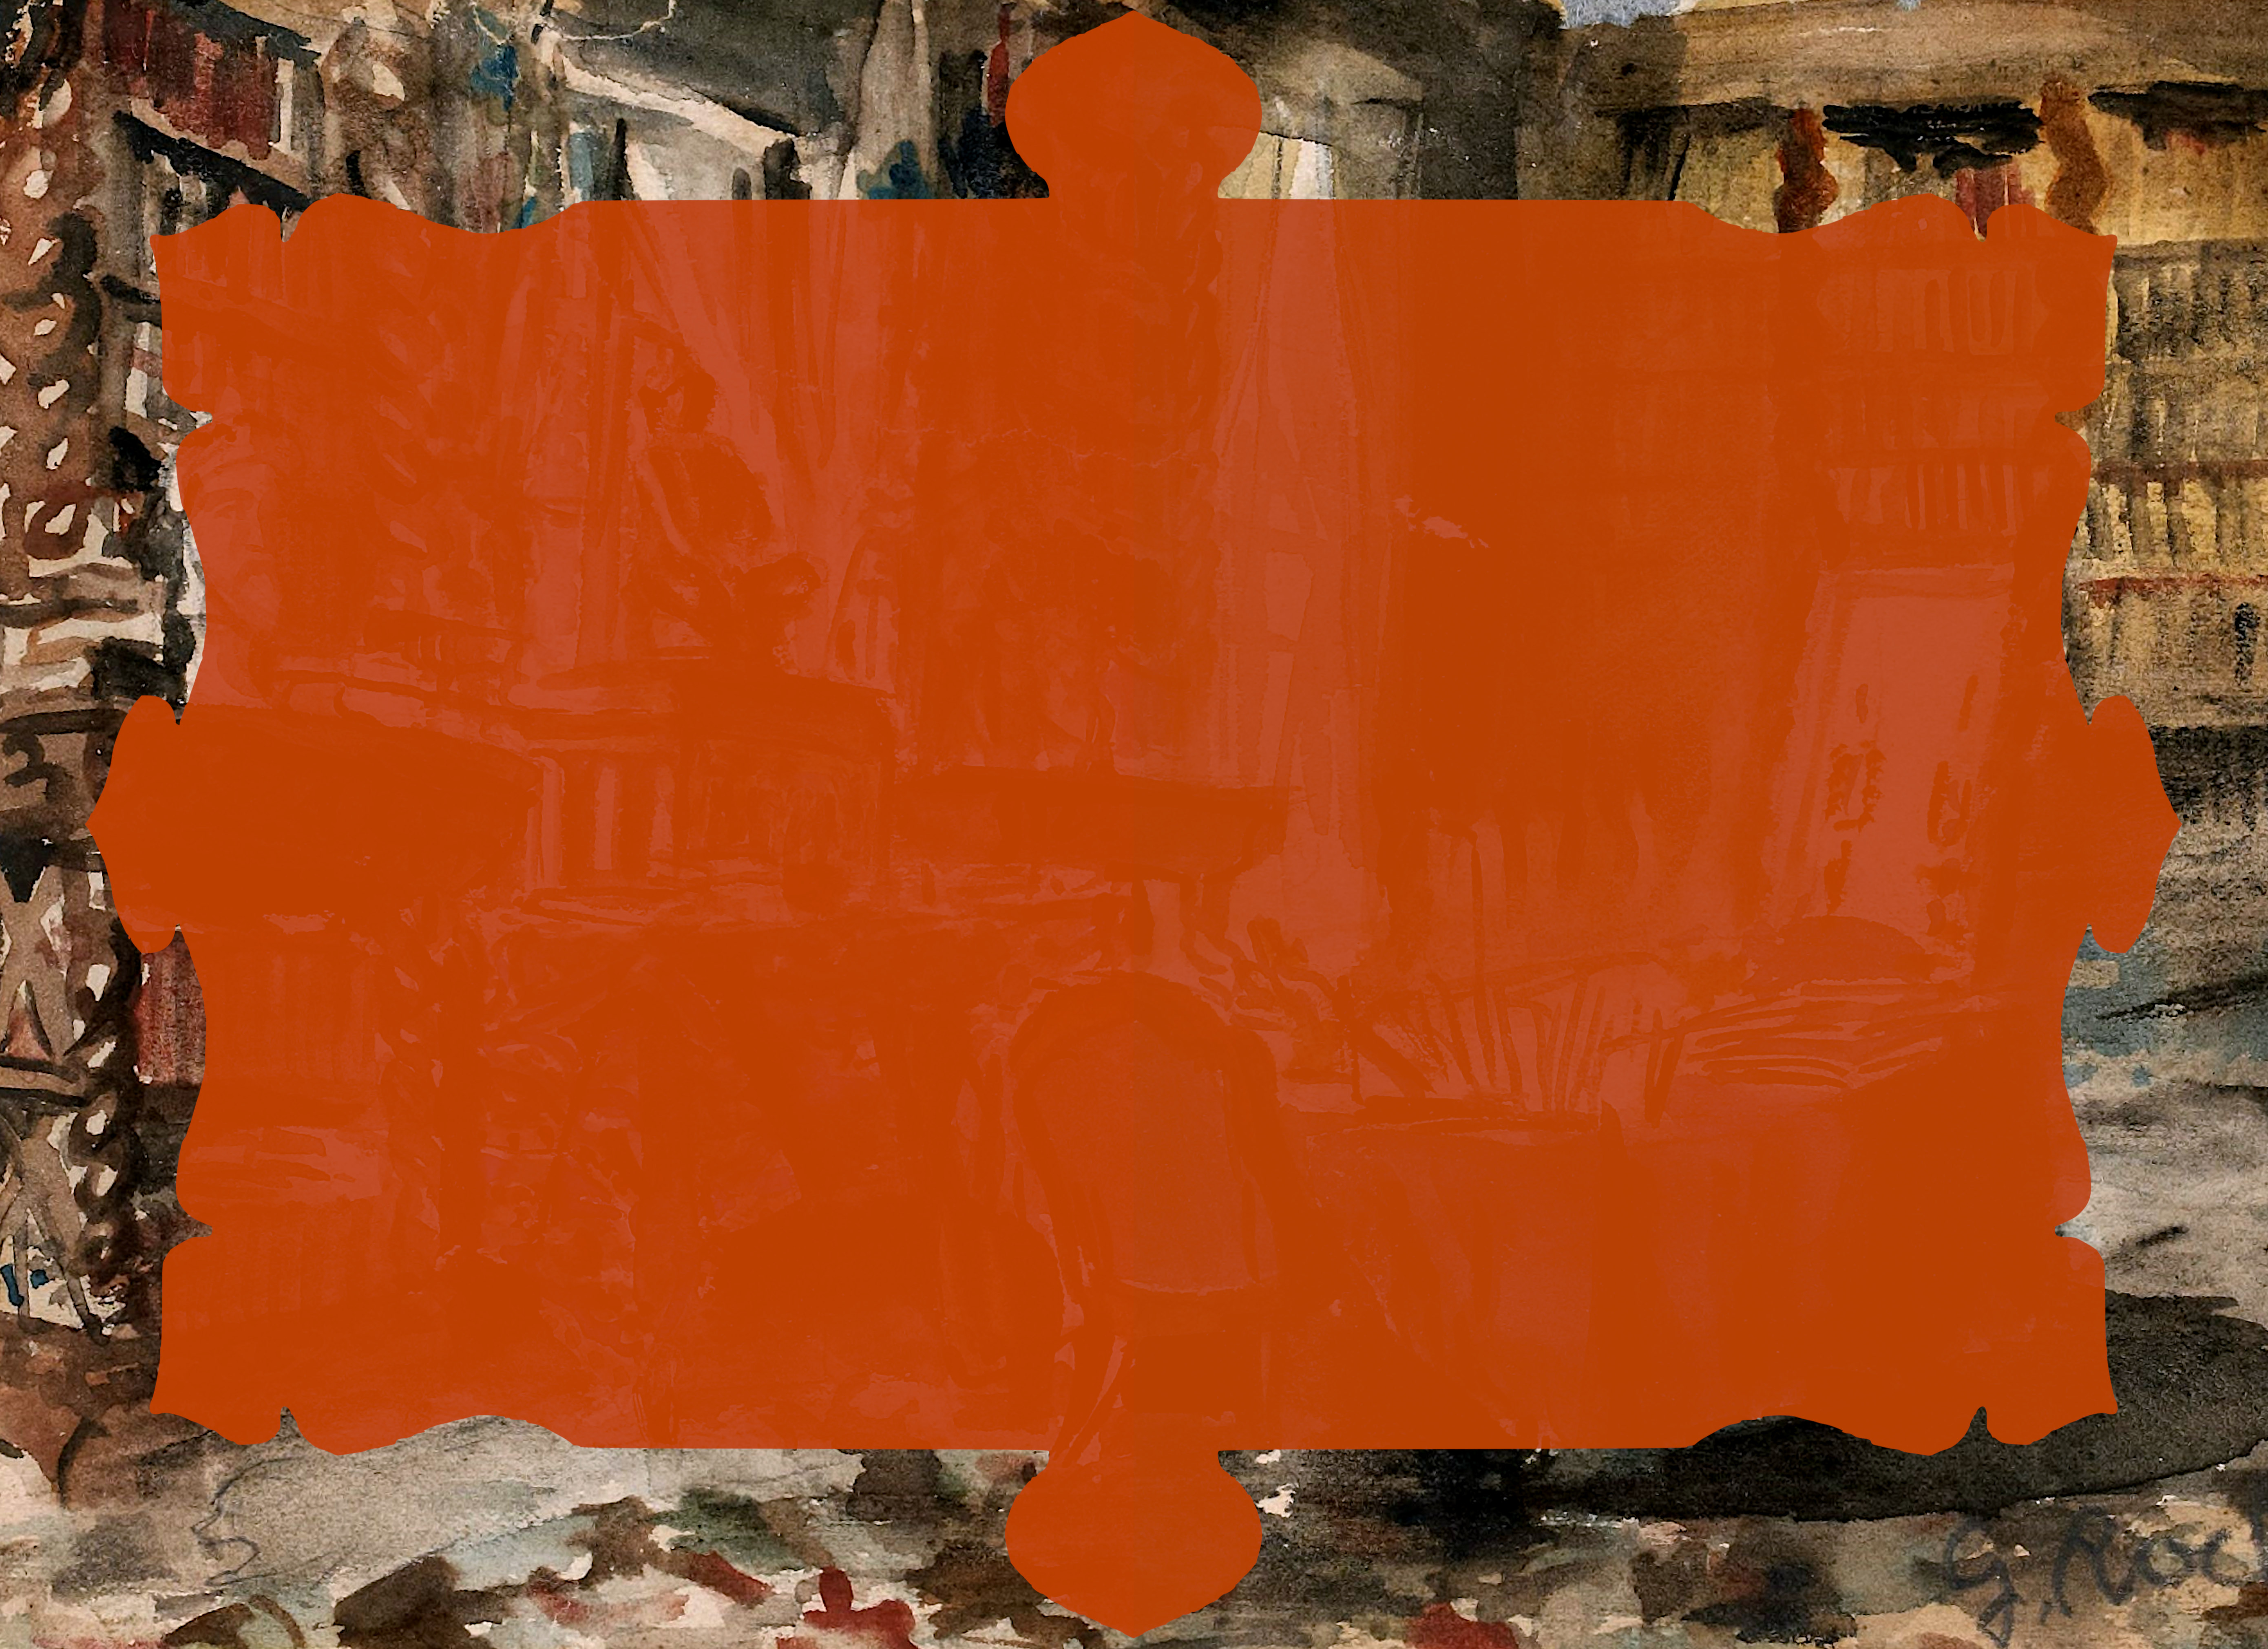
\includegraphics[width=\paperwidth,height=\paperheight]{Flaubert.jpeg}}
\begin{titlepage} % Suppresses headers and footers on the title page
	\centering % Centre everything on the title page
	\scshape % Use small caps for all text on the title page

	%------------------------------------------------
	%	Title
	%------------------------------------------------
	
	\rule{\textwidth}{1.6pt}\vspace*{-\baselineskip}\vspace*{2pt} % Thick horizontal rule
	\rule{\textwidth}{0.4pt} % Thin horizontal rule
	
	\vspace{0.5\baselineskip} % Whitespace above the title
	
	{\LARGE Mémoire Historique et Physique}

	\vspace{0.2\baselineskip}

	{\LARGE sur les Chutes des Pierres}

 	\vspace{0.2\baselineskip}

	{\LARGE Tombées sur la Surface de la Terre}

 	\vspace{0.2\baselineskip}

	{\LARGE a Diverses Époques.}
 
	\vspace{0.5\baselineskip} % Whitespace above the title

	\rule{\textwidth}{0.4pt}\vspace*{-\baselineskip}\vspace{3.2pt} % Thin horizontal rule
	\rule{\textwidth}{1.6pt} % Thick horizontal rule
	
	\vspace{0.5\baselineskip} % Whitespace after the title block
	
	%------------------------------------------------
	%	Subtitle
	%------------------------------------------------
	
	{Par M. P. M. S. Bigot de Morogues,\\ \footnotesize{Membré de la Société philomatique de Paris, de la Société minéralogique d'Jenna, de celle d'encouragement pour l'industrie nationale, de celles de Trèves, de Nantes, du Mans, et d'Orléans.}} % Subtitle or further description
	
	\vspace*{0.51\baselineskip} % Whitespace under the subtitle
	
	%------------------------------------------------
	%	Editor(s)
	%------------------------------------------------
    \vspace*{\fill}

	{\small\scshape }

    {Imprimerie de Jacob Ainé. Rue Bourgogne, n° 6.\\ Orléans, 1812.} % Subtitle or further description
    
    Internet Archive Online Edition  % Publication year
	
	{Utilisation non commerciale --- Partage dans les mêmes conditions 4.0 International} % Publisher
\end{titlepage}
\setlength{\parskip}{1mm plus1mm minus1mm}
\clearpage
\frenchspacing
\tableofcontents
\clearpage
\Large
\pagestyle{fancy}
\fancyhf{}
\cfoot{\Fontauri{\thepage}}
\section*{\Fontauri{Avis au Lecteur.}}
\paragraph{}
Lorsque j'entrepris cet ouvrage, je n'avois d'autre but que celui de comparer entr’elles les circonstances qui ont accompagné les chutes de pierres, afin de pouvoir déterminer celles qui semblent essentielles à ces sortes de phénomènes, et de les distinguer de celles qui n'ont pas constamment eu lieu ; ce qui selon moi était la seule méthode qui pût permettre d'essayer de connaître la cause de ces évènements aussi remarquables que communs.

Bientôt je me trouvai entraîné à des recherches qui me démontrèrent combien les ouvrages des meilleurs auteurs étaient incomplets sur la matière que je cherchais à approfondir, j'appréciai cependant leurs savants travaux et je n'osai entreprendre de donner un catalogue plus étendu que ceux qui avoient paru jusqu'à ce jour, que parce que j'étais à même de profiter des excellents écrits de ceux qui m'ont précédé à cet égard. La Lithologie atmosphérique d'Izarn, dont les citations m'ont paru très-exactes, les savants Mémoires de Chladni et ceux renfermés dans le Journal des mines, dans les Annales de chimie, dans celles du muséum, dans le Journal de physique, dans les recueils des Académies des sciences et des inscriptions et belles-lettres, ainsi que dans les Mémoires de l'Institut, m'ont été d'un grand secours. J'ai aussi consulté avec fruit le Bulletin de la Société philomatique de Paris, le Dictionnaire de chimie de l’Encyclopédie méthodique, celui de chimie de Klaproth et un grand nombre d'ouvrages relatifs à l'histoire ancienne ou moderne. Je dois encore témoigner ici ma reconnaissance à plusieurs savants célèbres qui ont eu la bonté de me communiquer des notes très-intéressantes ou de m'aider par leurs conseils ; je citerai parmi eux MM. Haüy, Cuvier, Gillet de Laumont, Tonnellier, Léman, Trémery, et Alluaud. Je les prie de vouloir bien agréer ici l'hommage de ma gratitude : je m'estimerai heureux si cet ouvrage peut mériter leur approbation et faciliter les recherches de ceux qui suivant les traces des de Laplace et des de Lagrange, essaieront de remonter jusqu'à la cause du phénomène important dont j'ai rassemblé ici les citations éparses dans un grand nombre d'ouvrages.

Je n'ai point osé, à l'exemple de plusieurs auteurs, me permettre de donner une théorie nouvelle ou renouvelée de toutes celles parvenues à ma connaissance. Celles des Comtes de Laplace et de Lagrange me paraissent les seules qui soient d'accord avec les circonstances relatives aux chutes de pierres ainsi qu'avec la nature de ces corps remarquables. Elles reposent à la vérité sur des bases qui au premier aspect nous paraissent inadmissibles ; mais chaque nouvelle découverte en physique a toujours semblé dans son principe aussi singulière. Ainsi lorsqu'un célèbre astronome nous démontra que la terre tournait autour du soleil, chacun crut d'abord qu'il déraisonnait ; on s'étonna de la hardiesse de Franklin, quand il nous apprit à diriger la foudre ; et quand Lavoisier retrancha l'eau du nombre des éléments, toute l'ancienne école le regarda comme un novateur aspirant à substituer des chimères à la place des opinions admises par tous les siècles, comme des vérités incontestables.

Nous-mêmes dans ces derniers temps, nous refusant à l'évidence et aux témoignages de toutes les nations, nous rangeâmes les chutes de pierres au nombre des préjugés populaires les plus absurdes : ne blâmons donc point les auteurs de théories savantes dont le calcul démontre la possibilité ; mais laissons dans l'oubli ces systèmes éphémères trop ordinairement le fruit de connaissances superficielles.
\clearpage
\section*{\Fontauri{Observations Préliminaires.}}
\paragraph{}
Le phénomène de la chute des pierres, si récemment révoqué en doute par les meilleurs auteurs, et maintenant admis par tous les savants comme incontestable, était connu dès la plus haute antiquité.

Les historiens chinois, ceux de la Grèce et de Rome nous l'ont attesté comme irrévocable ; ceux même du moyen âge nous ont transmis les relations d'un grand nombre de faits de ce genre ; mais dans les siècles derniers, la difficulté insurmontable de les expliquer, ou même de les mettre en rapport avec les autres faits connus, les fit regarder comme faux par la plupart des savants, qui, à cette époque, trouvèrent dans leur incrédulité l'excuse de leur ignorance. Bientôt les gens du monde et le peuple lui-même rangèrent au nombre des fables un des phénomènes les plus certains, dont la vérité était attestée par une multitude de témoignages irrécusables, chacun croyant alors, par ses doutes inconsidérés, faire preuve de la science qu'il n'avait point, et d'une prétendue force d'esprit, masque trop ordinaire de l'incertitude et de la faiblesse.

On peut cependant dire en faveur des modernes, qu'une des causes qui rendent excusable leur incrédulité sur la chute des pierres, est que ce phénomène rapporté par les anciens, se trouve ordinairement confondu par eux avec une foule de circonstances qui le rendent encore plus merveilleux; et que la superstition ou un zèle religieux se mêlèrent souvent à leurs écrits, ou parurent influer sur les traditions des peuples, qui regardèrent quelques-unes des masses tombées de l'atmosphère comme des objets divins.

C'est ainsi qu'il paraît démontré que la masse de pierre transportée à Rome du temps de Scipion-Nasica, et adorée sous le nom de mère des dieux, est réellement tombée du ciel ; et que le bloc de fer-natif trouvé en Sibérie, près des monts Kémir, entre Krasnojarck et Abakansk, et révéré par les Tartares, est d'origine céleste.

Du moment où la chute des pierres fut confondue avec les prodiges, les hommes, qui par leurs longues études se croyaient en droit de prétendre à une plus grande justesse de raisonnement, crurent devoir rejeter un fait, qui pour eux devenait contraire aux lois de la nature, et ne pouvait plus être considéré que comme une dérogeance à l'impulsion que lui imprima son divin auteur.

La raison autant que la religion éclairée des peuples modernes se refusèrent à admettre des miracles qui n'eussent eu aucun but d'utilité apparent, et qui par la même contrariaient si manifestement l'idée d'invariabilité inhérente à l'essence de l'être suprême.

Il est donc infiniment important de séparer le phénomène de la chute des pierres, de tous ceux avec lesquels il a été confondu par une foule d'auteurs d'ailleurs très-respectables, et de le réduire aux simples faits démontrés par l'expérience et par les dépositions des témoins les plus irrécusables.

C'est pour parvenir à ce but que je vais succinctement examiner ici les chutes de diverses substances étrangères à l'atmosphère, qui ont paru en tomber, et ont été quelquefois confondues avec les véritables aérolithes. La réalité de quelques-uns de ces phénomènes peut cependant être contestée, parce qu'ils peuvent être attribués à de trompeuses apparences ou à un examen peu approfondi de faits publiés tantôt par l'ignorance, tantôt par la mauvaise foi, et presque toujours trop légèrement admis.

Je ne parlerai pas ici des pluies de sang, des pluies de lait, de celles de chair, et autres semblables, qui ne paraissent nullement démontrées, ou ne sont que les résultats de l'illusion et de la mauvaise foi. Pline les indique dans le livre 2, chapitre 56, de son histoire du monde. Lemaire, dans son histoire des antiquités d'Orléans, rapporte qu'en juillet 1591, une pluie de sang est tombée à la Madeleine, près Orléans ; enfin beaucoup d'autres auteurs, et surtout les annalistes de chaque province, ont rapporté des évènements analogues. Les auteurs orientaux naturellement amis du merveilleux, en ont cité un grand nombre, et même ont parlé de pluies de grenouilles, de serpents, ou d'autres animaux vivants.

Tous ces faits ne paraissant pas constatés ou étant révoqués en doute, je ne les combattrai point, mais je renverrai ceux qui désireront plus de renseignements sur ce sujet, à l'excellent mémoire lu par Fréret, le 1$^{er}$ février 1717, à l'Académie royale des inscriptions et belles-lettres.

J'examinerai cependant particulièrement les divers phénomènes réunis dans un même tableau par le savant professeur Izarn, dans sa lithologie atmosphérique, afin de distinguer positivement les substances étrangères à la terre, qui tombent sur sa surface, de celles qui ont été détachées d'un des points de sa masse pour être rejetées sur un autre par une cause quelconque, et aussi pour séparer le phénomène de la chute des pierres, de ceux qui n'ont laissé après eux aucun corps de nature analogue.

Je retrancherai de ce même tableau ;

1° La pluie dont parle Dion, qui donna au cuivre l'apparence de l'argent, parce qu'il ne me paraît pas démontré, comme à Izarn, que cette pluie ait été de mercure, rien n'attestant la possibilité d'un pareil phénomène, et le peu de détails rapportés par Dion sur va fait aussi singulier, ne pouvant suffire pour établir une théorie à cet égard.

2° La chute du globe de feu qui, au rapport de Geoffroi, creva dans la place du Quesnoy, le 4 janvier 1717 ; parce qu'il ne lança aucune pierre, car ce fait, arrivé au centre d'une ville très-peuplée, eût été remarqué par ses habitants et par le savant qui en fit part à l'Académie royales des sciences.

On doit donc plutôt joindre ce phénomène à ceux analogues dont Chladni a rassemblé les citations en assimilant les chutes des bolides aux véritables chutes de pierres ; opinion que nous ne saurions admettre comme démontrée, mais qui cependant paraîtra toujours très-intéressante par la manière savante dont cet auteur l'a discutée. On peut la connaître non-seulement dans l'ouvrage original qui a été imprimé en allemand, mais encore dans l'excellente traduction de Coquebert, insérée au tome 15, page 286 et 446 du journal des mines.

On y remarquera que plusieurs des phénomènes qui y sont cités, pourraient être considérés comme ayant donné lieu à des chutes de pierres, car le bolide du 21 mai 1676, ayant éclaté au-dessus de la mer, près Livourne, ses fragments firent en tombant le même bruit qu'eût produit dans l'eau du fer rougi au feu. De même un autre bolide, vu en Italie le 22 février 1719, répandit, en faisant explosion, une odeur de soufre très-marquée. Il en est encore ainsi de celui dont quelques personnes crurent voir tomber les fragments dans l'Oder, et qui éclata en Silésie, le 19 février 1750. Enfin les fragments de celui qui, au rapport des Académiciens de Dijon, se dissipa le 11 novembre 1761, aux environs de cette ville, ayant été capables de mettre le feu à une maison sur laquelle ils tombèrent, il me semble probable qu'ils étaient réellement des corps solides et embrasés. Je ne rappellerai cependant pas ces quatre phénomènes dans l'ordre chronologique des chutes de pierres, attendu qu'il ne me paraît pas suffisamment démontré qu'il en soit tombé à leur suite.

3° Je retrancherai encore du mème tableau la pluie de sable tombée le 6 avril 1719, dans la mer Atlantique, de laquelle le père Feuillée montra un échantillon à l'Académie des Sciences. Comme ce sable était de nature analogue à celui du rivage voisin, on présuma qu'il avait pu être apporté par une trombe, phénomène ordinaire dans les pays sablonneux, dont tant de voyageurs furent victimes dans les déserts de l'Afrique, et dont le célèbre Bruce fut témoin avec un si terrible effroi.

Il est reconnu que les trombes d'eau ou de sable peuvent produire des effets surprenants, et que l'air, agité suffisamment pour les occasionner, enlève souvent des corps étrangers, mème très-solides ; mais rien ne démontre que les trombes aient le moindre rapport avec la chute des pierres, tombées si souvent par des temps calmes, ces dernières étant formées d'ailleurs d'éléments réunis dans des proportions différentes de celles déterminées dans tous les autres minéraux connus.

Le même raisonnement tend à démontrer que la chute des pierres n'a aucun rapport avec les éruptions volcaniques terrestres ; et, dans l'état actuel de nos connaissances, il serait absurde d'attribuer à la même cause, et l'épouvantable pluie de cendres qui engloutit pour jamais la malheureuse Pompeia, située au pied du Vésuve, et la chute des pierres tombées à l'Aigle ou à Charsonville, à une distance de plus de cent quarante myriamètres de tous les volcans en activité, lors même que ces volcans semblaient en repos ; d'ailleurs la nature des pierres tombées de l'atmosphère est tellement différente de celle des productions volcaniques connues, qu'il est parfaitement impossible d'établir aucune analogie entre les substances de ces deux origines.

En 1538, il tomba proche du village de Tripergola, en Italie, une pluie considérable de cendres et de pierres volcaniques. D'après le père Montfaucon, cette pluie eut lieu à la suite de tremblements de terre affreux ; l'air s'obscurcit par la grande quantité de poussière et de pierres dont il se remplissait sans cesse, lesquelles tombèrent pendant deux jours de suite, et formèrent une montagne au milieu du lac Lucrin.

Chacun connaît aussi l'épouvantable et sublime apparition de petites îles voisines de Santorini, dont l'une s'éleva, en 1707, du fond de la mer, dans l'Archipel, en vomissant une horrible quantité de pierres et de cendres embrasées qui se répandirent au loin. Mais ces sortes de phénomènes, évidemment volcaniques, n'ont nul rapport avec les chutes de pierres, ni par leur cause, ni par les circonstances qui les accompagnent, ni par la nature des pierres retombées sur la terre.

4° L'existence des pluies de soufre ou sulfureuses, rapportées par plusieurs auteurs dignes de foi, tels que Moïse, Spangemberg, Olaüs-Wormius et Siegesbek, et, d'après eux, par Van-Muscembroeck, ne peut guère être révoquée en doute ; mais ce phénomène, dont la cause était miraculeuse au rapport du premier auteur, et que nous ne connaissons pas encore assez parfaitement pour pouvoir l'expliquer sur le simple récit des trois suivants, ne nous paraît pas devoir être assimilé à la chute des pierres, qui sont de nature très-différente du soufre, dont elles ne renferment que quelques légères parties à l'état de combinaison ; et d'ailleurs les circonstances qui ont accompagné les trois pluies de soufre observées dans le duché de Mansfeld en 1658, à Copenhague en 1646, et à Brunswich en 1721, ne sont pas de nature à pouvoir être assimilées avec celles qui accompagnent la chute des pierres.

5° La pluie visqueuse qui, au rapport de Van-Muschenbroeck, tomba en Irlande en 1695, ne paraît pas non plus avoir aucun rapport avec le phénomène dont nous nous occupons ici.

6° La chute de la masse de feu observée en Amérique, dans la nuit du 5 avril 1800, paraît n'être que l'apparition d'un météore igné, analogue à celles qui eurent lieu dans une multitude d'endroits différents, et particulièrement au Quesnoy, en 1717, et dans le comté de Suffolk, en 1802.

Je mettrai dans ce mémoire, à l'exemple d'Izarn, la pluie de pierres qui eut lieu à Rome, sous le règne de Tullius-Hostilius, sur le mont Albanus, après la ruine d'Albe, ainsi que le rapporte Tite-Live, et celle qui eut lieu dans la même ville, sous le consulat de Caïus-Martius et Titus-Manlius-Torquatus, rapportée par Julius-Obsequens, attendu que ces deux pluies de pierres ne peuvent avoir été occasionnées par des éruptions volcaniques, quoique, par sa savante discussion, Fréret semble vouloir le faire eu pour témoin l'empereur Maximilien lui-même, est une époque assez remarquable pour se trouver le premier de cette section ; les historiens furent cependant encore presque les seuls à recueillir des récits dont les physiciens, alors trop prévenus, dédaignèrent de s'occuper.

Dans la fin de cette section, on verra la chute des pierres peu accréditée, n'être admise que par des observateurs trop peu célèbres pour entraîner l'opinion publique, ou trop peu hardis pour la braver. C'est ainsi que le savant Gassendi, rapportant un de ces faits, me put déterminer la croyance de ses contemporains dont il avait l'estime, et que Fréret, prêchant l'incrédulité, ne nous a transmis la série de quelques-uns de ces phénomènes, que pour essayer de les anéantir par ses raisonnements spécieux. Cet espace de temps, pendant la fin duquel les savants ou au moins ceux qui ambitionnaient ce titre glorieux, se faisaient un point d'honneur de ne s'occuper de la chute des pierres que comme d'un préjugé ridicule pu superstitieux, se prolongea jusqu'en 1768, temps auquel l'aérolithe tombé à Lucé, dans le centre de la France, fixa l'attention de l'Académie royale des Sciences.

Quoique les savants nommés par cette société célèbre pour en faire l'examen, s'efforçassent à chercher des explications maintenant inadmissibles, d'un fait dont ils ne pouvaient deviner la cause, ils eurent au moins la bonne foi et le courage de s'en occuper sérieusement ; et si le préjugé dont ils étaient imbus n'eût pas été aussi fort, il est probable qu'ils eussent admis la réalité de la chute de la pierre dont ils firent l'analyse.

C'est donc en 1768, dans le temps où tomba la pierre dont la chute fixa pour la première fois, l'attention de l'Académie, que je commencerai la troisième section de l'histoire de ces sortes de phénomènes, et je la continuerai pendant le temps où les savants, persistant à en nier la réalité, regardèrent cette croyance comme une absurdité digne d'être reléguée parmi les préjugés populaires.

La chute des pierres tombées à Bénarès en 1798, commencera la quatrième section. Par une de ces bizarreries de l'esprit humain que l'on ne saurait expliquer, ce phénomène arrivé dans l'Inde, fixa l'attention des savants de l'Europe, qui jusqu'à ce jour avoient dédaigné ceux de même genre dont leurs compatriotes avoient été les témoins oculaires ; la Société royale de Londres et l'Institut de France admirent alors, pour la première fois, sa possibilité, ou au moins jugèrent qu'on ne devait pas négliger l'occasion d'approfondir la vérité.

L'incertitude était cependant encore permise ; les savants partagés entr’eux, n'étaient pas également convaincus que des pierres tombassent réellement sur la surface du globe. Cette incertitude dura plusieurs années, et l'opinion n'était point irrévocablement fixée, lorsque la chute d'un très-grand nombre de pierres, arrivée à l'Aigle, au centre de la France, en 1803, put être vérifiée et constatée de la manière la plus authentique par les membres les plus éclairés de l'Institut de France.

C'est donc après la chute des pierres tombées à l'Aigle, que je commencerai ma cinquième section ; depuis cette époque, le doute n'est plus permis, et serait la preuve la plus évidente de l'ignorance la plus complète, ou du pyrrhonisme le plus absolu.

Les chutes qui eurent lieu postérieurement à celle-ci, se rangeront toutes dans cette cinquième section ; leur histoire sera particulièrement utile pour faire connaître la série des phénomènes qui accompagnent ces sortes d'évènements, et qui peuvent conduire par la suite à la connaissance presque certaine de leur cause. Jusqu'à ce jour, les savants partagés, non sur la réalité des faits, mais sur leurs explications, attendent sagement qu'une plus longue série d'observations et d'expériences bien faites, aient changé leur présomption en probabilité, ou même en certitude : puisse mon travail, à cet égard, leur être de quel qu’utilité. Quant à moi, me contentant dans ce mémoire de jouer le rôle d'historien, je rapporterai les diverses suppositions proposées jusqu'à ce jour, à mesure que la série des faits me le permettra, afin que ceux qui ne sauraient croire que ce qu'ils peuvent expliquer, choisissent celle qui leur paraîtra la plus convenable ; et n'en regardant aucune comme parfaitement démontrée, je me garderai bien d'émettre une opinion nouvelle, étant parfaitement convaincu qu'une mauvaise théorie ne pourrait être considérée que comme un rêve, et que si les savants les plus célèbres de l'Europe ne sont parvenus qu'à prouver que leurs explications ne sont pas complètement improbables, il me serait impossible de faire mieux.

Enfin, je terminerai ce mémoire par une sixième section, destinée 1° à faire connaître les principales substances que l'on présume tombées sur la terre, sans en savoir les époques ; 2° à analyser les faits relatifs au phénomène dont nous nous occupons ici ; et 3° à conclure définitivement ce qui doit nous paraître constant ou variable, et démontré ou incertain dans l'état actuel de nos connaissances.

Dans la discussion relative à la suite chronologique des faits rapportés dans cet ouvrage, et particulièrement dans la première section, je ne m'étendrai que peu sur la plupart d'entr'eux, souvent même, lorsqu'ils n'auront occasionné aucune observation importante, je ne ferai que les énoncer, en renvoyant ceux qui désireront de plus amples renseignements, aux ouvrages originaux desquels ils ont été extraits. D'ailleurs il eût été inutile, et souvent même impossible, d'entrer dans de plus grands détails à leur sujet ; par-là je n'eusse fait que répéter ce qui se trouve dans d'autres parties de mon ouvrage, et je l'eusse grossi inutilement de redites ennuyeuses du moment où elles ne seraient plus nécessaires.

Au contraire, dans la deuxième partie ainsi que dans les suivantes, j'entrerai dans de très-grands détails sur certains faits, afin que le rapprochement des témoignages d'une multitude d'individus très-éloignés, et souvent inconnus les uns des autres, puisse servir non seulement à constater la vérité d'une manière plus authentique, mais encore faire connaître l'ensemble des phénomènes qui se manifestent constamment lors de la chute des pierres, et les différences qui peuvent exister dans quelques circonstances.

Le but que je me suis proposé dans ce long mémoire, sur une suite de faits qui ne sont plus douteux, est,

1° De faire connaître une série de chutes de pierres bien constatées, plus complète que celles publiées jusqu'à ce jour ;

2° De distinguer ce phénomène de ceux avec lesquels il a pu être confondu ;

3° De démontrer combien est commun un phénomène que naguère nous regardions comme une absurdité évidente ;

4° De faire observer combien il est long et difficile de faire croire les faits les plus certains, lorsqu'ils nous paraissent inexplicables ;

Et 50 de faire remarquer à combien d'erreurs la chute des pierres a donné lieu, et quel parti avantageux la politique a su quelquefois en retirer.
\clearpage
\section{\Fontauri{Première Section.}}
De toutes les pluies de pierres, la plus mémorable et la plus anciennement constatée, est sans contredit celle dont Dieu se servit pour détruire l'armée des cinq rois chananéens, que Josué venait de mettre en fuite près de Gabaon, l'an 1451 avant notre ère. Voici ce qui est rapporté à ce sujet au verset 11, chapitre 10 du livre de Josué :

\og Lorsqu'ils fuyaient, le Seigneur fit tomber du ciel de grosses pierres sur eux jusqu'à Azeca, et cette grêle de pierres qui tomba sur eux, en tua beaucoup plus que les enfants d'Israël n'en avait passé au fil de l'épée. \fg

Ce fait miraculeux, au moins par ses effets, par le lieu, et le moment, semble à dom Calmet être le même déguisé, dans la fable qui rapporte qu'Hercule faisant la guerre aux fils de Neptune, obtint de Jupiter une pluie de cailloux, qui écrasa ses redoutables ennemis.

Je le cite ici, étant parfaitement convaincu que ceux même qui se croiraient en droit de récuser une autorité aussi respectable que celle des livres saints, seront toujours obligés d'admettre que le phénomène de la chute des pierres était connu dès la plus haute antiquité, et dans le temps où le livre de Josué fut écrit. Ils admettront même comme probable, que vers cette époque une chute considérable de pierres eut lieu dans un pays voisin de la Judée, et frappa singulièrement l'imagination des peuples de l'Asie, puisque les Hébreux et les peuples voisins en conservèrent simultanément la mémoire dans leurs traditions et dans leurs écrits.

Attendons quelques temps encore, et peut-être que beaucoup de faits consignés dans les ouvrages des anciens, qui naguère nous paraissaient totalement miraculeux, ne nous paraitront plus aussi complètement contraires aux lois de la nature.

On doit mettre au nombre des pierres tombées, dont il est fait mention dans l'histoire sous les dates les plus anciennes, sans pouvoir en assigner l'époque d'une manière précise, la pierre adorée jadis, et désignée sous les noms d'Elagabale, chez les Phéniciens, et de Cybèle ou mère des dieux, chez les Phrygiens, et peut-être de Jupiter-Amon, dans la Lybie.

On sait que ces dieux n'étaient originairement autre chose qu'une grosse pierre noire de forme pyramidale, que l'on croyait tombée du ciel ; ne pouvait-on pas présumer que la vue d'un phénomène aussi extraordinaire que la chute d'une énorme masse de pierre, tombant toute embrasée avec un fracas épouvantable, en aura pu imposer assez aux peuples grossiers et superstitieux de l'ancienne Phrygie, pour leur faire adorer cette masse brute comme un dieu.

Ce culte était très-ancien, car les Egyptiens eux-mêmes, dès l'an 660 avant J.-C., sous le règne de Psammeticus, avoient reconnu la haute antiquité des Phrygiens, et personne n'ignore que dans les temps très-reculés les hommes étaient enclins aux superstitions les plus grossières. Leur histoire, dans ces premières époques, se trouve enfouie dans une multitude de circonstances mensongères, elle est pour nous un problème presque insoluble, et ce n'est qu'en tâtonnant, que l'on parvient à rencontrer quelques rapprochements heureux, susceptibles d'y jeter quelques faibles rayons de lumière. Il nous paraît donc probable que les Phrygiens et les Phéniciens adorèrent simultanément une masse de pierre qu'ils virent tomber du ciel ; l'intérêt politique qui tendait à réunir les hommes encore errants, dut singulièrement favoriser leur croyance, et les prêtres de leurs dieux ne laissèrent point échapper cette occasion d'augmenter leur pouvoir.

Bientôt le culte de la divinité envoyée du ciel, se répandit de proche en proche, les mystères et les cérémonies qui y furent annexés, accrurent le nombre de ses partisans, la vénération croissant d'âge en âge, le rendit de plus en plus respectable, et les dieux de la Phrygie, de l'Egypte, de la Phénicie, et de la Grèce, utiles partout aux besoins de la politique, devinrent par la suite ceux de Rome et de presque tout l'univers ; c'est ainsi que la mère des dieux, transportée avec pompe, exigea partout des miracles pour soutenir ses autels, et qu'enfin les Romains crédules admirèrent l'impure Claudia, faisant entrer dans leur port le vaisseau chargé de leur nouvelle divinité, qui en lui rendant l'honneur, devait à la fois faire et sa fortune et celle des prêtres qui l'avoient corrompue.

Cette masse tombée du ciel à Pessinunte, dans la Phrygie, était adorée sous les noms d'Ida et de mère des dieux, lorsque les Romains envoyèrent des députés à Attale 1$^{er}$, roi de Pergame, pour la lui demander. Publius-Scipion Nasica, connu par sa vertu, fut choisi par le Sénat, quoique fort jeune, pour aller la recevoir, et le culte de cette divinité grotesque s'établit dans Rome, l'an 204 avant J.-C.

Le savant Biot lut un mémoire sur ce sujet à la société philomatique en juillet 1791. Et maintenant il est parfaitement reconnu que la mère des dieux était une véritable bœtylie ; mais le temps de sa chute ne peut être fixé d'une manière certaine, quoique l'on sache parfaitement qu'elle eut lieu à une époque très-reculée, et de beaucoup antérieure à celle de la chute de la pierre tombée proche le fleuve Ægos-Potamos.

Au rapport d'Arnobe, cette pierre était d'un volume médiocre, de couleur noire, et de substance anguleuse et métallique ; un oracle avait annoncé aux Romains que la prospérité de l'empire irait toujours croissante, s'ils parvenaient à se procurer ce précieux dépôt ; et le Sénat intéressé au maintien de la superstition, se servit de ce moyen pour la ranimer.

C'était aussi un semblable motif qui faisait conserver, près du temple de Delphes, une autre pierre du même genre, qui, d'après Pausanias, passait pour avoir été rejetée par Saturne, et être tombée dans la Grèce ; ainsi la politique habile savait profiter alors des phénomènes extraordinaires pour créer des miracles, et attacher à son sol, par la superstition, un peuple encore grossier et à demi-barbare.

Tite-Live rapporte, dans le § 31 du livre 1$^{er}$ de ses décades, la chute de pierres dont l'époque est la plus anciennement constatée dans l'histoire profane, il nous apprend que la guerre des Sabins étant glorieusement terminée (environ 654 ans avant J.-C.), on vint annoncer au roi et au Sénat qu'il était tombé une pluie de pierres sur le mont Albanus. Comme on avait peine à croire une pareille chose, on envoya sur les lieux, pour s'en assurer, et ceux qui s'y portèrent virent effectivement tomber du ciel des pierres aussi pressées que la grêle, lorsque les vents la chassent sur la terre. Les Romains, en expiation de ce prodige, qu'ils regardaient comme d'un sinistre présage, ordonnèrent des sacrifices solennels pendant neuf jours, usage qui se perpétua toutes les fois qu'on vit arriver le même évènement.

Non-seulement ce phénomène fut regardé comme un prodige véritable par le peuple superstitieux de Rome, mais les philosophes eux-mêmes, et l'incrédule Cicéron en particulier, l'ont rapporté comme étant convaincus de sa réalité.

Le savant dom Calmet, qui s'est occupé de rassembler à ce sujet les citations des anciens, rapporte que quelques temps après la bataille de Cannes (216 ans avant J.-C.), on vit sur la même montagne d'Albe, une pluie de pierres qui dura deux jours de suite.

La même chose s'est fait remarquer à divers endroits, par exemple, à Aricia, à Capoue, à Rome, à Lavinium, à Amiternes, et dans la marche d'Ancone ; quelquefois c'était de simples pierres qui tombaient, d'autres fois des pierres enflammées, et quelquefois de la terre.

Il est très-fâcheux que les détails donnés par les auteurs anciens sur ces divers phénomènes, soient trop peu circonstanciés pour nous apprendre positivement s'ils doivent être rapportés à la même cause que les chutes de pierres dont nous sommes journellement les témoins. Il est souvent impossible de déterminer, d'après leurs récits, si ces faits doivent être attribués à une cause volcanique, comme on doit le faire pour la pluie de cendre qui tomba à Constantinople l'an 472, et pour celle qui, en 1537, s'étendit jusqu'à cent lieues des côtes de Sicile, et dut son existence à une éruption du mont Ætna ; ou si on doit attribuer la chute des pierres qu'ils ont dit être tombées sur la terre, à un violent orage arrachant les rochers du sommet des montagnes, et les précipitant dans les vallées, ainsi qu'Hérodote et Justin rapportent que cela eut lieu aux approches du temple de Delphes.

La chute de pierres la plus ancienne, parmi celles consignées dans les histoires de la Chine, paraît être celle de cinq pierres tombées dans le pays de Song, 644 ans avant notre ère. De Guignes en fait mention dans le tome 1$^{er}$ de son voyage, page 195, où il dit que la seizième année du règne de Hy-Kong, dans le printemps, à la première lune, au jour Von-Chin, quarante-cinquième du cycle, il tomba du ciel cinq pierres dans le pays de Song.

Dom Calmet a observé, dans ses commentaires, que Malchus, dans la vie de Pythagore, parle d'une pierre de foudre. Si on doit croire qu'elle tomba en Crète du temps de ce philosophe, on pourra présumer que sa chute eut lieu pendant ses voyages, c'est-à-dire, environ 520 ans avant J.-C.

Vers la seconde année de la soixante-dix-huitième olympiade, environ 467 ans avant notre ère, on vit tomber du ciel une grande pierre proche le fleuve Ægos en Thrace ; le poète Pindare, né en Béotie, vivait à cette époque, il est donc présumable que cette pierre fut celle qui tomba à ses pieds. Comme c'était aussi dans ce même temps que florissait Anaxagore, il est également probable que la prédiction qu'il fit de la chute de cette pierre ne fut faite qu'après coup, pour frapper davantage l'esprit crédule des anciens habitants de la Grèce, Pline nous apprenant que l'on croyait que ce philosophe avait indiqué le jour où elle devait être détachée du corps même du soleil, et tomber sur la terre.

Il attribue aussi au même Anaxagore une autre prédiction semblable, relativement à la chute de la pierre qui était conservée à Abidos avec un respect religieux.

Il est très-remarquable que la pierre tombée près la rivière des Chèvres ou Ægos-Potamos, qui se voyait encore du temps de Pline, ait été aussi exactement décrite par lui ; car cet auteur rapporte qu'elle tomba en plein jour, qu'elle était de la grosseur d'un chariot, et que sa couleur était comme si elle avait été brûlée (\emph{colore adusto}). Il dit aussi qu'au temps de cette chute, il parut une comète, qui dura assez longtemps, mais il ne parle pas d'explosion, et ne rapporte pas si la comète disparut aussitôt après, ce qui eût été important à connaître pour juger si ces deux phénomènes avoient quelque connexion entr'eux. On doit même remarquer que si le globe de feu qui apparaît souvent lors de la chute des pierres avait été pris dans ce cas pour une comète, il serait très-singulier qu'il eût duré aussi longtemps que le rapporte Pline.

Il est cependant très-remarquable que Plutarque, dans la vie de Lisandre, donne des détails du même phénomène, qui en confirment la réalité, et en rendent l'époque certaine, puisqu'il dit que, vers le temps de la victoire que ce général remporta sur les Athéniens, proche la rivière des Chèvres, il tomba du ciel une grande et grosse pierre, qui de son temps était encore très-révérée dans la Chersonèse.

D'après le rapport des anciens auteurs, cette chute fut précédée, pendant soixante-quinze jours de suite, par l'apparition d'un grand corps lumineux, ressemblant à une nuée enflammée dans une agitation continuelle, et jetant des feux semblables aux météores vulgairement appelés \emph{étoiles tombantes}. Les habitants du lieu, après s'être rassurés, s'approchèrent de l'objet qui avait causé leur effroi, et ne trouvèrent point de feu, mais une pierre qui quoique grande, l'était cependant beaucoup moins que le corps lumineux ne le paraissait.

Pline nous apprend encore qu'il était tombé une autre pierre à Cassandrie, ville de Macédoine, où sa présence regardée comme d'un favorable augure, attira une puissante colonie. Cette ville, située dans l'isthme qui joignait Pallène à la Macédoine, portait originairement le nom de Potidée, qui signifie en grec \emph{être brûlée}, probablement à cause de la couleur brûlée et enfumée de la pierre dont la politique se servit pour y fixer des habitants. On doit donc croire que cette pierre était très-anciennement tombée, et qu'elle était encore conservée dans l'ancienne Potidée, lorsque le roi Cassandre, ayant rebâti cette ville vers l'an 315 avant notre ère, lui imposa son propre nom.

Une autre pierre tombée du ciel était aussi conservée dans le gymnase d'Abydos, ville de l'Asie mineure, sur le Bosphore de Thrace ; Pline, qui rapporte qu'elle y avait été reçue précieusement, ne nous dit point quand elle tomba, et n'indique pas le lieu de sa chute ; on peut cependant présumer que ce fut postérieurement au sixième siècle avant J.-C., car la ville d'Abydos avait été brûlée par Darius, 508 ans avant notre ère, lorsque ce roi vaincu par les Scythes et fuyant dans ses états, craignit d'être poursuivi par ce peuple belliqueux ; d'où nous pouvons conclure que la pierre dont parle Pline, avait été apportée dans le gymnase de la ville qui fut reconstruite sur les ruines de l'ancienne Abydos, postérieurement à son rétablissement.

Valère-Maxime, livre 1, chapitre 6, rapporte que, sous le consulat de C. Volumnius et Ser. Sulpitius, on fut témoin de divers prodiges, entr'autres d'une pluie de pierres ; comme il ne dit relativement à cet évènement, que, \emph{in Piæno lapides pluisse}, je ne le cite ici que pour n'omettre aucun des faits parvenus à ma connaissance. Je remarquerai seulement, que dans les fastes consulaires, on trouve que l'an de Rome 293, qui correspond à l'an 461 avant J.-C, P. Volumnius-Amintinus-Gallus et Cer. Sulpitius-Camerinus étaient consuls ; c'est donc à cette époque qu'il me paraît convenable de placer les prodiges que Valère-Maxime a dit être arrivés dans le temps de ce consulat, et en particulier cette pluie de pierres, sur laquelle je n'ai trouvé aucun autre renseignement, sinon qu'elle eut lieu, vers cette époque, dans la marche d'Ancône.

Julius-Obsequens rapporte que sous le consulat de Caïus-Martius 3 et Titus-Manlius-Torquatus (l'an 410 de Rome, ou 343 ans avant J.-C.), il tomba une pluie de pierres si considérable, que le ciel en fut obscurci, et qu'elle cacha la lumière aux habitants de la ville Rome.

De Guignes, qui a compulsé les ouvrages des anciens auteurs chinois, nous apprend dans son voyage, que l'an 211 avant notre ère, sous le règne de Chy-Hoang-Ty, une étoile tomba jusqu'à terre, et se convertit en pierre ; ce qui me semble démontrer que cette chute fut accompagnée de lumière.

Quoi qu'il en soit, ce phénomène frappa singulièrement les contemporains, car les habitants du lieu, voulant en profiter pour donner une leçon à l'empereur, firent graver ces paroles sur la pierre : \og Chy-Hoang-Ty est prêt de mourir, et son empire sera divisé ; \fg ce qui l'irrita tellement qu'il fit massacrer tous les habitants des environs de l'endroit où se trouva la pierre, et la fit briser ensuite.

Cette cruauté lui fut funeste, car il mourut à la septième lune de l'année d'après ; et sous le règne de Eul-Chy-Hoang-Ty qui lui succéda, l'empire se révolta, fut divisé en une multitude de royaumes ; et la dynastie des Tsin finit deux cent sept ans avant J.-C., et trois ans après la mort de Chy-Hoang-Ty.

Le savant voyageur, de l'ouvrage duquel j'ai extrait ces détails, rapporte que cent quatre-vingt-douze ans avant J.-C., il tomba une autre pierre dans le même empire.

Il rapporte encore que quatre-vingt-neuf ans avant J.-C., à la deuxième lune, au jour Ting-Yeou, trente-quatrième du cycle, il tomba deux pierres à Yong, et que cette chute fut accompagnée d'un tel bruit, qu'elle fut entendue jusqu'à quatre cents ly (quarante lieues) de distance ; le temps était, dans ce moment, calme et sans aucun nuage apparent.

Pline, que malgré notre incrédulité nous consulterons toujours avec fruit, rapporte qu'il tomba en Lucanie une pluie de fer spongieux. Cet auteur ne fait mention ni d'aucun globe de feu, ni d'aucun autre météore apparu dans cette circonstance, il dit seulement qu'elle eut lieu l'année d'avant la défaite de Crassus par les Parthes, qui, d'après J. Blair, arriva l'an 52 avant J.-C.

On trouve dans le livre 5 des commentaires de César, concernant la guerre d'Afrique, qui eut lieu 46 ans avant notre ère, qu'à-peu-près dans le temps de la levée du siégé d'Acilla, il s'éleva, vers la seconde veille de la nuit, un violent orage avec une grêle de cailloux, dont les troupes souffrirent beaucoup, parce qu'elles n'avoient ni tentes ni casernes pour se mettre à couvert ; les ténèbres et l'eau les désolaient, la nuit était extrêmement obscure, et les soldats couraient de tous côtés en se couvrant la tête de leurs boucliers.

De Guignes, que nous avons déjà cité, indique dans son voyage en Chine plusieurs chutes de pierres qui eurent lieu dans ce pays, durant l'espace des trente-huit dernières années qui précédèrent notre ère.

Ainsi, la trente-huitième année avant J.-C., il tomba six pierres dans le pays de Leang, à la première lune, au jour Vouchin, cinquième du cycle, et l'an 29 avant J.-C. ; à la première lune, dans le printemps, il tomba du ciel quatre pierres, à Pô, et deux dans le territoire de Tchin-Ting-Fou ; dans le printemps de l'an 22 avant J.-C., il tomba du ciel huit autres pierres ; et ce phénomène se renouvela l'an 19 avant J.-C., car il tomba encore trois autres pierres vers la cinquième lune.

Au rapport du même auteur, l'an 15 avant J.-C., à la deuxième lune, il tomba une étoile en forme de pluie. Ce fait doit-il être classé parmi les chutes de pierres, qui souvent ont été accompagnées de lumière ? ou doit-on l'assimiler aux chutes de feu arrivées au Quesnoy, à Suffolk, et à Lessay ? c'est ce que la courte citation de de Guignes ne peut nous apprendre, mais comme il peut appartenir au phénomène de la chute des pierres, dans l'incertitude, j'ai cru devoir le citer ici.

Les auteurs chinois, consultés par de Guignes, ont encore consigné dans leurs ouvrages les chutes de pierres suivantes. L'an 12 avant J.-C., il tomba une pierre à Tou-Kouan, à la quatrième lune : le ciel étant clair, on entendit un bruit comme de plusieurs coups de tonnerre ; une grande étoile, longue de dix Tchang (cent pieds), blanche et brillante, venant du sud-est, et suivant le soleil, parut sous la forme d'une pluie de feu, et s'arrêta le soir au coucher du soleil.

Enfin, l'an 9 avant J.-C., il tomba également du ciel, dans l'empire de la Chine, deux pierres, et, l'an 6 avant J.-C., ce phénomène se renouvela deux fois ; car, à la première lune, il tomba seize pierres dans le pays de Ning-Tcheou, et, à la neuvième lune, il en tomba deux autres à Yu.

Il est fâcheux que le travail de de Guignes, duquel j'ai extrait ces diverses citations, n'ai pas été prolongé dans des temps postérieurs à la naissance de Jésus-Christ et surtout que les ouvrages chinois qu'il a consultés, n'aient pas donné de plus grands détails sur les phénomènes qui ont accompagné les diverses chutes de pierres desquelles ils nous ont transmis les dates.

Il paraît présumable que la pierre vue par Pline dans la terre des Vocontins, où elle était depuis peu de temps, était tombée près de là, à une époque peu éloignée de celle où il la vit. Comme cet auteur célèbre périt dans les flammes du Vésuve l'an 79 de notre ère, on peut donc placer au commencement de cette époque la chute de la pierre dont il est ici question.

L'an de Grâce 452, il tomba du ciel, dans la Thrace, trois grosses pierres. On trouve ce fait consigné dans la chronique du comte Ammian-Marcellin, ainsi que l'a observé Chladni dans son catalogue ; mais ce savant a omis d'y inscrire le fait suivant qu'on remarque parmi les fragments que Photius, auteur du neuvième siècle, nous a conservés de la vie d'Isidore, écrite par Damascius, où il nous apprend que ce philosophe, vivant dans le sixième siècle, avait vu des pierres tomber du ciel sur le mont Liban, et que cette chute avait été accompagnée d'un globe foudroyant et lumineux.

Ce récit renfermé dans la Bibliothèque de Photius, page 1047, est accompagné d'une foule d'absurdités qui prouvent à quel point, dans ce siècle d'ignorance, des jongleurs adroits savaient abuser de la crédulité du vulgaire. On trouve surtout à la page 1062 du même ouvrage, le détail des fourberies par lesquelles un médecin nommé Eusèbe, sut s'attirer une grande vénération en montrant une de ces pierres.

Comme l'ouvrage de Photius, que je cite ici, est fort rare, et que les morceaux de Damascius, dont j'ai extrait ce fait, m'ont paru curieux par leur originalité, j'ai cru devoir les rapporter ici dans leur entier. On doit observer, en les traduisant, que l'auteur a employé les mots \emph{betulia}, \emph{bætula}, et \emph{betulus}, à la place de \emph{betylus}.

Voici le texte de Photius, édition de 1653 (\emph{Rothomagi}), page 1047, article de Damascius :

\og \emph{Juxtà Heliopolim Syriæ, ait Asclepiadem in montem Libani ascendisse, et vidisse multa betulia vel bœtula, de quibus multa prodigiosè dignaque impio ore prosequitur, dicitque se et Isidorum hœc posteà vidisse.} \fg

Voici encore à ce sujet le texte de Photius, page 1062 :

\og \emph{Videram, inquit, bætulum,} ... \emph{Nomen medici, qui bœtulum gestabat, erat Eusebius, qui etiam dixit accidisse sibi aliquandò nec opinanti subitum impetum errandi ab Emessâ urbe, penè mediâ nocte, quam longissimè ad montem illum in quo Palladis templum veteri magnificentiâ conditum est, et ivisse sese celerrimè ad cacumen montis, et ibidem tanquam è via fessum desedisse, et vidisse globum ignis celeriter decidentem, et leonem ingentem in globo constitutum, et illum statim evanuisse : seque, igne jam extincto, ad globum cucurisse, et illum tanquàm bœtulum accepisse, et rogasse cujus dei esset, et respondisse illum esse Gennœi Gennœum Heliopolitæ colunt, erecta quadam leonis forma in templo Jovis. Ivisse, eâdem nocte, viâ non minùs quàm decem et ducentorum stadiorum, ut aiebat, continuò. Eusebius non erat dominus bætuli motuum, ut alii aliorum, sed hic petebat, et orabut : ille verò locum dabat oraculis. Hæc, et multa similia, nugatur dignus profectò bœtuliis lapidibus : quin etiam formam ejus describit : globus quidem, inquit, egregius, colore subcandido, diametro longus palmo, sed interdùm major apparebat, interdùm minor, interdùm purpureus, et litteras ostendit nobis in lapide descriptas, idque colore tingabarino, ut vocant, et in muro fixit. Undè sciscitanti oraculum dedit, et vocem emisit è tenui fistulâ, quam interpretatus est Eusebius. Vanæ mentis ille alia multa miranda de bætulo narrat. Equidem putaram diviniùs esse oraculum bœtuli, Isidorus dæmonium potiùs esse dixit. Esse enim aliquem dæmonem moventem illum, non unum ex admodùm malis, non omninò immateriatis, nec omninò puris : bætulorum alium alii incumbere, ut ille criminans dicit, deo, Saturno, Jovi, Soli, et aliis.} \fg

Quatremère, dans le tome 2 de ses mémoires sur l'Egypte, indique, page 486, une pluie de poussière, qui, d'après la chronique syriaque d'Edesse, eut lieu l'an 742. Comme je ne connais aucun détail sur cet évènement, je le cite ici quoiqu'il ne me paroisse pas certain qu'il doive se rapporter au phénomène de la chute des pierres.

On trouve dans l'abrégé chronologique de l'histoire de France par Mézerai (Amsterdam, 1696, tome 1$^{er}$, et dans l'édition in-4°, Paris, 1668, tome 1$^{er}$), que l'an 823, la naissance de Charles-le-Chauve fut présagée par un grand nombre de prodiges, entr'autres, par une pluie de gros carreaux de pierre qui tombèrent avec de la grêle, et que des hommes et des bestiaux furent en quantité d'endroits frappés de la foudre.

Ce fait me paraît pouvoir être rapporté au phénomène de la chute des pierres, et c'est pour cette raison que je le place ici, quoique l'histoire de France du même auteur (édition de 1643 à 1651, trois volumes infolio) n'en fasse mention que comme d'une grêle extraordinaire ; mais on sait que l'abrégé chronologique de Mézerai passe pour plus exacte que sa grande histoire, et que la première édition de ce dernier ouvrage n'est plus recherchée que les autres qu'en raison des opinions hardies qu'elle renferme, et qui ne se trouvent point dans les éditions subséquentes, attendu que l'auteur fut forcé de les supprimer ; mais quant aux faits, Mézerai mit de plus en plus d'exactitude, et l'abrégé fait par lui est par cette raison préférable à son grand ouvrage.

D'ailleurs ce fait se trouve encore confirmé par le père Bonaventure de Saint-Amable, qui rapporte dans les annales du Limousin, volume 3, page 305, que dans l'année 823, en Saxe, vingt-trois villages furent embrasés par le feu du ciel, et que dans la campagne les hommes et les bêtes furent assommés par de grosses pierres mêlées avec la grêle.

Quatremère rapporte, dans le tome 2 de ses mémoires sur l'Egypte, que l'auteur du Mirat-Al-Zeman nous apprend, d'après Ibn-Habib Al-Haschemi, que ce fut au mois de safar de l'année 238 de l'hégire, que Taher-Ben-Abdallah envoya au calife Montawakkel une pierre tombée du ciel dans le Tabarestan, qui pesait huit cent quarante dirhems.

Cette chute de pierre arriva donc vers le mois de safar de l'année 238 de l'hégire, c'est-à-dire, vers la fin de juillet, et avant la fin du mois d'août 852 de J.-C.

On trouve dans les mêmes mémoires, qu'au rapport d'Ibn-Al-Athir, en l'année 285 de l'hégire (c'est-à-dire, du 28 janvier 898 au 17 janvier 899 de notre ère), on éprouva dans la ville de Koufah un vent chargé de vapeurs jaunes, qui continua à souffler jusqu'au coucher du soleil ; alors il changea, et prit une couleur noire ; bientôt après il tomba une pluie violente, accompagnée de coups de tonnerre effrayants, et d'éclairs qui se succédaient sans interruption ; au bout d'une heure il tomba, dans un village appelé Ahmed-Dad, et dans les environs, des pierres blanches et noires, dans le milieu desquelles étaient des rugosités. On en porta plusieurs à Bagdad, où elles furent vues de beaucoup de personnes.

L'an 318 de l'hégire (du 3 février 930 au 24 janvier 931), on vit, à Bagdad même, une rougeur dans le ciel, et il tomba sur les toits des maisons quantité de sable rouge. Ce phénomène me semble plutôt dû à une trombe de sable qu'à une véritable chute de pierres.

D'autres évènements analogues, arrivés postérieurement à cette époque, sont cités par Chladni d'après plusieurs auteurs dignes de foi ; ainsi il rapporte, d'après Platine, que, sous le pape Jean 13, c'est-à-dire, de 965 à 971, il tomba une pierre en Italie ; et il cite encore, d'après Avicenne, deux autres chutes analogues arrivées l'une à Lurgea ou Lorge, et l'autre à Cordova en Espagne, mais il ne fait pas mention de celle arrivée dans le Djordjan, quoiqu'elle soit rapportée par le même auteur.

Abou-Ali-Houssain Ben-Abdallah, philosophe et médecin arabe, plus connu sous le nom d'Avicenne, né l'an de l'hégire 370 (du 17 juillet 980 au 7 juillet 981 de notre ère), a écrit sur beaucoup de sujets différents, et a consigné dans ses ouvrages plusieurs chutes de pierres ; il cite entr'autres une masse de fer très-dur, du poids de plus de vingt-quatre kilogrammes, qui tomba à Lurgea. Le même auteur vit une autre pierre sulfureuse qui était tombée à Cordova en Espagne ; et enfin il cite une masse considérable de fer grenu qui tomba dans le Djourdjan ou Djordjan, ainsi que nous l'apprend cet auteur, cité par Aboul-Feda. \og De mon temps, dit ce célèbre écrivain, il tomba de l'atmosphère, dans la province de Djordjan, une masse qui pesait environ cent cinquante mann ; étant arrivée à terre, elle rebondit comme une balle lancée contre un mur, et retomba ensuite ; sa chute fut accompagnée d'un bruit épouvantable : plusieurs personnes étant accourues pour en savoir la cause, trouvèrent cette masse, qu'elles portèrent au gouverneur du Djordjan. Mahmoud-Ben-Sebektekin, sultan du Khorasan, manda à cet officier de lui envoyer sur-le-champ, ou la totalité, ou une partie de la pierre. Comme sa pesanteur en rendait le transport impossible, on voulut en casser un morceau, mais la dureté du métal était si grande, qu'elle faisait briser les outils ; en sorte que ce ne fut qu'avec la plus grande peine que l'on parvint à en détacher un fragment, qui fut envoyé au sultan. \fg

\og D'après les ordres de ce prince, on essaya d'en forger une épée, mais on ne put jamais y parvenir. Suivant ce que l'on m'a raconté, ajoute Avicenne, cette masse était composée de petits grains ronds, semblables à du millet, et unis les uns aux autres. \fg

J'ai extrait ces derniers détails des mémoires sur l'Egypte par Quatremère. Ils m'ont paru d'autant plus curieux, que les caractères assignés par Avicenne à la pierre tombée dans le Djordjan, sont parfaitement convenables à plusieurs de celles de ces mêmes masses que nous avons vu tomber dans les derniers temps ; ce qui nous prouve la véracité de l'auteur arabe, contemporain de ces phénomènes, qui par conséquent arrivèrent antérieurement à 1036, année dans laquelle mourut ce savant célèbre.

En 998, il tomba deux grandes pierres, l'une dans la ville de Magdebourg, et l'autre dans un champ voisin, situé sur les bords de l'Elbe. Spangenberg, qui cite ce fait dans la Chronique saxonne, rapporte que ces pierres tombèrent pendant un orage.

L'an 464 de l'hégire (correspondant à la fin de 1071 et au commencement de 1072), dit l'auteur du Mirat-Al-Zeman, il tomba dans l'Irak une pluie accompagnée de grêle et de boules de terre, qui ressemblaient à des œufs de moineaux, et avoient une odeur agréable.

Cette chute, dont Quatremère a fait mention, ne me paraît nullement avérée, tant à cause des circonstances qu'il cite, que par la nature même des boules de terre, qui ne paraissent avoir aucun rapport avec les pierres tombées de l'atmosphère à cause de leur odeur agréable ; je l'indique cependant en raison de la difficulté de se procurer des détails sur les faits de ce genre aussi anciennement arrivés, et parce que d'ailleurs nos connaissances relatives à la chute des pierres, sont encore trop peu avancées pour que nous puissions assurer connaître toutes les variétés des substances tombées sur la terre. Il me paraîtrait donc téméraire de rejeter absolument les faits de ce genre, que nous ne saurions encore assimiler à ceux que nous connaissons d'une manière positive.

En 1136, à Oldisleben, en Thuringe, il tomba une pierre de la grandeur d'une tête humaine. (\emph{Spangenberg, Chr. Sax.})

En 1164, le jour de la fête de la Pentecôte, il tomba une pluie de fer en Misnie. (\emph{Georg. Fabric. rer. Misn.})

Ces derniers faits se trouvent cités par Chladni, et sont connus de tous les savants ; mais je ne sache point que dans les catalogues des chutes de pierres, aucun auteur ait cité celle que rapporte Henri Sauval dans l'histoire des antiquités de Paris, où il dit, d'après Rigord, qu'en juin 1198, il fit une telle tempête à deux lieues de Paris, entre Chelles et Tremblai, que tout fut renversé, et que même il tomba des pierres, les unes grosses comme des noix, les autres comme des œufs, ou même davantage.

On trouve aussi, dans la Chronique saxonne de Spangenberg, qu'en 1249 il tomba des pierres aux environs de Quedlimbourg, Battenstad, et Blankembourg, et qu'en 1304 il en tomba beaucoup d'autres à Friedberg, près la Saal.

Quatremère, que j'ai déjà cité, rapporte encore, d'après Macrizy, que le premier jour du mois de Moharram, de l'année 723 de l'hégire (correspondant au 10 janvier 1323), à la suite d'une pluie et d'un vent violent, il tomba dans les provinces des Mortahiah et de Dakhahiah, une grêle, dont les grains pesaient plus de cinquante dirhems ; laquelle fut accompagnée de pierres, dont plusieurs pesaient de sept à trente rotls, qui détruisirent un grand nombre de bourgs, et tuèrent une multitude de bœufs et de moutons.

On trouve dans les annales du Limousin, par le père Bonaventure de Saint-Amable (vol. 3, p. 607), qu'en 1305, le jour de Saint-Remi, au sol des Vandales, il tomba de la grêle dans laquelle il y avait des pierres embrasées de feu, qui causèrent plusieurs incendies.

La plupart des faits précédents ne sont indiqués que d'une manière vague, mais cependant rien ne porte à croire qu'ils doivent être rapportés à d'autres causes que les phénomènes analogues dont nous sommes journellement les témoins ; mais il n'en est pas de même du fait suivant.

En 1438, il tomba des pierres spongieuses près de Roa, non loin de Burgos en Espagne. Proust cite à ce sujet, dans le Journal de physique, tome 60, la lettre écrite par Chibdadréal, dans laquelle ce fait mémorable est rapporté de la manière suivante :

\og Le roi dom Juan et sa cour, étant à chasser au bas de la côte du village de Roa, le soleil se cacha sous des nuages blancs, et l'on vit descendre de l'air des corps qui ressemblaient à des pierres grises et noirâtres, d'un volume très-considérable... Après une heure que dura ce phénomène, le soleil reparut... Un champ, qui n'était pas éloigné d'une demi-lieue, était tellement couvert de pierres de toutes grandeurs, qu'on ne distinguait pas le terrain. Le roi voulut s'y transporter, mais on l'en empêcha, et on lui rapporta quatre pierres d'une grandeur considérable ; les unes étaient rondes et du volume d'un mortier, d'autres comme des oreillers de lit, et comme des mesures de demi-fanègues ; mais ce qui causait le plus d'étonnement, c'était leur excessive légèreté, puisque les plus grandes ne pesaient pas une demi-livre. Elles étaient si tendres, qu'elles ressemblaient plus à de l'écume de mer condensée qu'à toute autre chose. On pouvait s'en frapper le dedans des mains sans crainte d'y causer ni contusion, ni douleur, ni la moindre apparence, \emph{etc.} \fg

Il résulte évidemment de ce récit que les pierres tombées près de Roa étaient d'une nature différente de celles qui ont été examinées dans ces derniers temps ; il me semble même que leur chute ne devrait pas trouver place dans ce catalogue, et je ne la rappelle ici que parce qu'il paraît que ces masses spongieuses sont tombées de l'atmosphère ; je n'ai fait en cela que suivre l'exemple du savant professeur Chladni : mais j'avoue que pour regarder ce phénomène comme parfaitement constaté, il me semblerait important de pouvoir le rapprocher de quelques autres qui lui soient analogues.

C'est ici que je vais terminer cette première section, qui sera toujours, pour la science, l'époque de l'incertitude. Une foule d'absurdités évidentes, ou de mensonges grossiers, ayant accompagné le récit des évènements qui s'y trouvent consignés ; il est difficile d'en induire aucune conséquence exacte qui puisse servir à déterminer la cause du phénomène dont nous nous occupons ici ; mais cependant nous pourrons en conclure plusieurs vérités importantes :

1° Que le phénomène de la chute des pierres a eu lieu très-souvent ;

2° Qu'il a eu lieu dans tous les temps, et même dans les siècles les plus reculés dont les monuments historiques nous aient conservé le souvenir ;

3° Qu'il a eu lieu dans tous les pays, et a été observé chez tous les peuples civilisés ;

4° Qu'il a frappé d'autant plus les peuples qui en ont été les témoins, que l'intérêt et la politique surent en profiter ;

5° Qu'enfin, embelli par la mauvaise foi ou par la superstition, il a été regardé comme un prodige par les auteurs qui n'en ont pas nié la réalité, jusqu'au milieu du quinzième siècle, temps auquel va commencer la seconde section de l'histoire de ce phénomène remarquable.
\clearpage
\section{\Fontauri{Deuxième Section.}}
\paragraph{}
Un des faits les plus remarquables et les mieux constatés, parmi les nombreuses chutes de pierres qui eurent lieu dans les derniers siècles, est la chute de la pierre tombée à Ensisheim le 7 novembre 1492, près Maximilien 1$^{er}$, alors roi des Romains, et depuis empereur, en 1493. Dans un rescrit, daté d'Ausbourg, le 12 novembre 1503, ce prince cite cette pierre, qu'il dit être tombée près de lui, lorsqu'il était à la tête de son armée, à laquelle il la donna comme un présage de la victoire qu'il allait remporter contre les Français. Brant fit de ce phénomène le sujet de quelques poésies ; et quelques auteurs ont attribué à ce fait extraordinaire le changement qui s'opéra à cette époque dans la conduite de Maximilien. C'est donc par erreur que Muschenbroeck, dans ses Essais de physique, indique cette chute comme arrivée en 1630.

Voici un extrait de la traduction littérale d'une notice allemande sur la pierre d'Ensisheim, qui se trouvait autrefois avec elle dans l'église paroissiale de ce lieu.

\og L'an 1492, le 7 novembre, arriva un miracle singulier, car entre les onze heures et midi, il advint un grand coup de tonnerre, et un long fracas qu'on entendit à une grande distance, et il tomba dans le bourg d'Ensisheim, une pierre pesant deux cent soixante livres. Un enfant la vit frapper dans un champ situé dans le banc supérieur, vers le Rhin et l'In, près du canton dit Gisgaud, où elle fit un trou de plus cinq pieds de profondeur. On en détacha d'abord des morceaux, ce qui fut défendu par le Landwogt, et elle fut transportée dans l'église comme un objet miraculeux. \fg

\og Le bruit s'était entendu à Lucerne, à Villing, et en beaucoup d'autres endroits, avec tant de force, qu'on crut que des maisons venaient d'être renversées. Le roi Maximilien, étant à Ensisheim, fit porter au château la pierre qui était tombée avec tant de fracas, et défendit d'en ôter aucun morceau, hors deux, dont il garda l'un, et envoya l'autre au duc Sigismond d'Autriche, et enfin il ordonna de la suspendre dans l'église où on la voyait attachée avec une chaîne à la voûte du chœur. \fg

\emph{Irithemius in Chronico Hirsangiensi M. S.}, écrit en 1590, rapporte ce fait, et dit que dans le village Simtgaw, auprès du bourg d'Ensisheim, non loin de Bâle, en Allemagne, il tomba, le 7 novembre 1492, une pierre pesant deux cent cinquante-cinq livres, qui se cassa en deux morceaux, dont on voyait de son temps le plus considérable suspendu, avec une chaîne de fer, à la porte de l'église d'Ensisheim.

On trouve aussi le même fait, rapporté par Paulus-Lang \emph{in Chronico Cizizense}, où il dit également que, le 7 novembre 1492, il s'éleva un orage durant lequel le ciel parut tout en feu, et que tandis que le tonnerre grondait, il tomba, près le bourg d'Ensisheim, une pierre d'une grosseur prodigieuse, avec un fracas horrible.

Cette pierre était de la forme triangulaire d'un \emph{delta}. Au rapport de J. Lintarius, son poids était de trois cents livres et plus ; elle était dure et de différentes couleurs, et tomba, avec un très-grand bruit, d'un nuage brillant et enflammé, tandis que le reste de l'horizon n'offrait aucun autre nuage ; il ajoute que dans ce moment, le ciel étant toujours serein, on aperçut autour de la lune une grande \emph{croix rouge}.

On peut voir que, dans ces deux derniers récits, le fait commence à prendre une tournure merveilleuse, et que les circonstances différentes de la première relation conservée dans l'église même d'Ensisheim, en deviennent d'autant moins prouvées. D'ailleurs ces derniers historiens n'étaient ni témoins oculaires, ni même contemporains. Il est d'abord contradictoire que le premier rapporte qu'il s'éleva un orage pendant lequel le ciel parut tout en feu, et que le dernier dise au contraire que la pierre tomba d'un nuage brillant et enflammé, tandis que le reste de l'horizon n'offrait aucun nuage ; il est d'ailleurs très-remarquable que la relation annexée à la pierre ne fasse aucune mention ni du ciel en feu, dont parle Paul Lang, ni du nuage enflammé, d'où Lintarius a fait sortir la pierre ; aussi M. de Drée classe-t-il cette chute de pierre parmi celles qui ont eu lieu par un temps serein et sans tonnerre.

Quoi qu'il en soit, il est certain qu'un morceau de la pierre dont il est ici question, pesant cent soixante-onze livres, fut conservé et suspendu, jusqu'à la révolution, dans l'église d'Ensisheim, et transporté depuis dans la bibliothèque publique de Colmar.

Le professeur Bartholdt fut le premier qui eut l'avantage de fixer l'attention des savants modernes sur cette pierre, qu'il ne décrivirent qu'après lui. Elle est d'une couleur gris-bleuâtre ; renfermant des portions de pyrite jaunâtres, et d'autres de fer de couleur grise ; sa cassure est irrégulière, grenue, un peu terreuse, et fendillée ; elle ne fait point feu au briquet ; sa contexture est lâche ; elle se laisse entamer au couteau, et se réduit en poussière d'un gris-bleuâtre et d'une odeur terreuse ; et enfin elle renferme quelques particules métalliques qui résistent au pillon : sa pesanteur spécifique est de 3,2332.

Je ne rapporterai pas l'analyse qu'il en fit, attendu que les expériences de Vauquelin et Fourcroy en ont démontré la fausseté. Les conclusions qui la terminent ne sont pas plus exactes, car Bartholdt, après avoir regardé comme fabuleuse l'origine de cette pierre, la compare à une espèce de roche de corne, dans son mémoire qui a été imprimé dans le tome 50 du Journal de physique.

M. de Drée, savant minéralogiste, qui a publié dans un mémoire très-intéressant la plupart des détails que je viens de donner sur cette pierre, remarque que sur les échantillons qui lui furent envoyés par M. F. Despotes, préfet du département du Haut-Rhin, on reconnaît la croûte noir-brunâtre, vitrifiée dans les espèces de cavités qui ont été à l'abri du choc et du frottement ; et que cette pierre renferme des grains de fer malléable contenant du nickel ; du sulfure de fer lamelleux, blanchâtre, en rognons et en grains ; et du sulfure de fer gris moins sulfuré, en couches minces, écailleuses, tapissant une multitude de petites fissures qui traversent la pierre en tous sens.

Les caractères de la pierre d'Ensisheim sont d'être d'un gris d'ardoise sans éclat, renfermant des parties lamelleuses brillantes ; sa structure est celle d'un gneiss schisteux, composé de parties pierreuses grenues, d'un gris-blanchâtre, entremêlée de feuillets minces d'une substance fissile d'un gris d'ardoises, et de grains de fer pur et de fer sulfuré ; ce dernier se voit aussi en lames superficielles sur les feuillets gris, sa contexture est granulaire et fissile, sa cassure est inégale sur la tranche, et plus lamelleuse dans le sens des feuillets. Cette pierre est tenace, aride au toucher, et sans odeur argilleuse ; enfin elle fait varier l'aiguille aimantée, et essayée au chalumeau, la substance grise se noircit et se fritte.

Sage rapporte, dans le journal de Physique, qu'il possède un échantillon de cette pierre renfermant une veine de nickel, remarquable par sa couleur gris-rougeâtre ; il met l'alumine au nombre de ses éléments.

Mais Fourcroy, dans un rapport fait par Vauquelin et lui, à la séance publique de l'Institut, le 28 fructidor an 11, après avoir remarqué que la pierre d'Ensisheim, renferme de petits filons de sulfure de fer et de nickel gris et brillant, observe qu'il n'y a pas rencontré de globules de fer très-sensibles ; et nous apprend que cent parties lui ont donné à l'analyse,
\begin{table}[H]
    \centering
    \Fontauri
    \bfseries
    \large
    \begin{tabular}{l r}
        Silice & 56 \\
        Fer oxidé & 30 \\
        Magnésie & 12 \\
        Nickel & 2,4 \\
        Soufre & 3,5 \\
        Chaux & 1,4 \\ \hline
        Total & 105,3 \\
    \end{tabular}
\end{table}
\paragraph{}
Les 5,3 d'augmentation doivent être attribués à l'oxydation du fer pendant l'opération. Depuis cette analyse, Klaproth à découvert un cinquième pour cent d'alumine dans cette pierre, ainsi qu'on le voit dans le tome 70 des annales de chimie.

On trouve dans le bulletin de la société Philomatique de mai 1810, qu'en 1496, le 28 janvier, il tomba trois pierres entre Cezena et Bartonari. Ce fait est consigné dans l'ouvrage de Sabellicus. (\emph{Hist. ab urbe conditâ. Enneas 10. Lib. 9. Parisiis 1513, tom. 2, f. 341.})

Un autre fait de même genre se trouve aussi indiqué par Mercati dans le chapitre 19 du livre 15 de son ouvrage, intitulé \emph{Metallotheca Vaticana} : il y est dit que la chute d'une pierre eut lieu dans le pays qui borde l'Adda, peu d'années auparavant la grande pluie de pierres de 1510, de laquelle il va être question.

Cardan rapporte, au sujet de cette dernière, qu'en 1510, on vit tomber du ciel, près Crema, non loin de la rivière Adda en Italie, une grande pluie de pierres, dont le nombre fut d'environ douze cents. Une d'elle pesait cent vingt livres, une autre soixante, et les autres un peu moins. Avant leur chute, il avait paru un grand feu en l'air qui avait duré près de deux heures. Elles tombèrent avec sifflement comme d'un tourbillon enflammé ; elles avoient la couleur brune du fer, une odeur sulfureuse, et étaient une dureté extraordinaire.

Sans prétendre infirmer ici le récit de Cardan, qui me paraît d'autant plus exacte que les caractères qu'il assigne à ces pierres se rapportent très-bien à ceux des autres pierres tombées du ciel, je crois devoir observer qu'il est singulier que dix-huit ans après l'évènement arrivé à Ensisheim, et dans un temps où ce fait mémorable était encore si récent, la pluie de douze cents pierres, en un seul lieu, ait fait si peu de bruit dans le monde savant, à l'époque où Laurent de Médicis, surnommé le Père des Lettres, les avait naguère rendues si florissantes, dans cette même Italie, où Cardan rapporte que ce fait eut lieu, et dans le temps même où vécurent l'Arioste, Machiavel, et tant d'autres gens célèbres. Je crois donc que l'on peut présumer, sans témérité, que le fait avancé par Cardan a été augmenté, et que toutes ses circonstances ne sont pas exactes, surtout l'apparition d'un grand feu, qu'il dit avoir été vu en l'air deux heures de suite ; espace de temps qui ne s'accorderait nullement avec les faits de ce genre constatés jusqu'à ce jour. Ce fait se trouve cependant rapporté de la même manière dans le \emph{Metallotheca Vaticana} de Mercati, qui dit que l'on porta de ces pierres à la cour de France.

Mercati rapporte aussi qu'il tomba, dans une plaine entre Cicuic et Quivira, dans la nouvelle Espagne, des pierres de la grandeur de coins ; fait qui se trouve confirmé par Cardan, dans le livre 17 de son ouvrage, intitulé \emph{de rerum Varietate}, dont l'édition originale fut imprimée en 1557 ; d'où nous conclurons que ce phénomène est antérieur à cette époque, quoiqu'il fut alors très-récent, la province de Honduras dans laquelle il eut lieu, n'ayant été découverte qu'en 1502 par Christophe Colomb, lors de son quatrième voyage. Il est donc évident que cette chute doit être placée vers le commencement du seizième siècle.

Je ne puis cependant m'empêcher d'observer ici que ce fait n'est rien moins qu'avéré, car le savant voyageur Humboldt observe dans une note (tome 4, page 107, de l'édition in-8° de son Essai politique sur la nouvelle Espagne), que l'on ignore aujourd'hui la position géographique de Cicuic et de Quivira, et que ces noms rappellent les fables du Dorado de l'Amérique méridionale : j'ai cependant cru devoir indiquer cette prétendue chute de pierres, parce que Cardan, Mercati, et Chladni l'ont citée.

Le père Bonaventure de Saint-Amable rapporte le fait suivant (Ann. du Limousin, vol. 3, pag. 746) : \og a le 4 septembre 1511, à Crême, en Lombardie, pendant un orage épouvantable, il tomba dans la plaine des pierres d'une grosseur considérable ; six de ces pierres pesaient cent livres. On en porta une à Milan, qui pesait cent dix livres. Leur odeur était semblable à celle du soufre. Des oiseaux furent tués en l'air, des brebis dans les champs, et des poissons dans l'eau. \fg

Il me parait évident que ce fait est le même que celui que Cardan rapporte comme arrivé en 1510. Ce dernier auteur, écrivant sur les lieux, et peu de temps après cette chute dont il fut contemporain, on doit croire que la date qu'il donne est plus exacte que celle rapportée par le père Bonaventure.

Au surplus, cette époque fut féconde en phénomènes de ce genre, car, d'après Albini Mesnische, il tomba au commencement du seizième siècle, une grande masse de fer dans une forêt près de Neuhof, entre Leipsick et Grimme ; et le père Bonaventure de Saint-Amable rapporte (Annales du Limousin, vol. 3, pag. 769) le fait suivant : \og L'an 1540, le 28 avril, il y eut une violente tempête, accompagnée de tonnerre et de grêle ; elle dura dix jours, dévastant les différentes contrées du Limousin. Dans la paroisse des Eglises, il tomba avec la grêle une pierre plus grosse qu'un baril, qui entra dans la terre à la profondeur de deux aunes, et on la retira de ce trou avec des barres de fer. Il tomba aussi plusieurs autres pierres grosses comme des œufs. \fg

Ce rapport paraît d'autant plus vrai, que les autres faits de même nature cités par le même auteur, sont rapportés semblablement par d'autres historiens, à quelques très-légères différences près dans les dates.

Il me parait donc qu'on doit ajouter foi à cette citation, qu'Izarn et Chladni n'ont point indiquée dans leurs ouvrages. M. Alluaud, savant minéralogiste, auquel je dois la connaissance de ce fait, se propose de faire des recherches à ce sujet dans la paroisse des Eglises, peu éloignée de Limoges où il fait sa résidence habituelle. Il serait bien curieux que le hasard lui fît rencontrer quelques-unes des pierres citées par le père Bonaventure, près de trois siècles après leur chute.

Mercati nous apprend que dans une partie du Piémont, on vit tomber du fer du ciel, trois ans environ avant l'époque où le duc de Savoie, père d'Emmanuel, fut dépouillé de ses états par le roi de France, et où il les recouvra par le secours de l'empereur Charles-Quint ; ce qui détermine le temps de cette chute de 1540 à 1550.

Beaucoup d'autres faits semblables eurent lieu dans ce même temps, car d'après Spangemberg, le 6 novembre 1548, il tomba à Mansfeld, en Thuringe, une masse noirâtre.

Et le même auteur rapporte que le 19 mai 1552, il y eut beaucoup de dégâts occasionnés aux environs de Schleusingen, en Thuringe, par une pluie de pierres, desquelles l'auteur apporta quelques-unes à Eisleben.

Chladni rapporte encore (d'après \emph{Nic. Isthuanhi. Hist. Hungar.}) qu'il tomba en 1559, cinq pierres ou masses de fer, près de Miskoz, en Transilvanie, pendant une horrible tempête accompagnée de tonnerre et d'une grande commotion de l'air. La grosseur de ces pierres, dont quatre sont conservées au trésor de Vienne, est à-peu-près celle de la tête d'un homme ; elles sont très-lourdes, leur teinte est le jaune pâle couleur de rouille, et elles répandent une odeur de soufre très-forte. J'observerai à ce sujet que probablement ce dernier caractère est inexactement rapporté dans l'excellent mémoire de de Drée, attendu qu'il est bien vrai que les pierres qui tombent sur la terre répandent une forte odeur au moment de leur chute, mais qu'elles ne la conservent pas longtemps ; aussi Chladni dit-il qu'elles sentaient fortement le soufre, et non pas qu'elles le sentent maintenant.

Anselme Boèce de Boot rapporte, dans le livre second, chapitre 260 de son Traité des pierres et pierreries, que plusieurs personnes dignes de foi assurent avoir trouvé des pierres de tonnerre à l'endroit même où le coup avait frappé ; il dit, entr'autres choses, que Keutmannus raconte qu'il tomba une pierre (\emph{ceraunia}) à Torga, le 17 mai 1561, laquelle étant tirée de terre, était de la largeur de trois doigts, et longue de cinq, et plus dure que le basalte dont on se sert en divers lieux d'Allemagne en guise d'enclume.

Le même auteur rapporte que proche la citadelle Julia, il trouva une pierre de même nature qui était tombée sur un grand chêne, et que dans le bourg de Siplitz, une seconde pierre tomba sur une autre chêne, d'où elle fut retirée et donnée en présent au questeur de Torga.

Boèce de Boot a tiré cette citation de l'ouvrage de Conrad-Gesner, auteur estimé, qui rapporte avec exactitude la chute de la pierre tombée à Ensisheim en 1492 : on peut donc la regarder comme véritable.

J'observerai ici que la dureté de la pierre tombée à Torga, paraît devoir faire présumer qu'elle était très-métallique et probablement de l'espèce des masses de fer natif reconnues de même origine ; au surplus on sait que souvent les pierres tombées présentent une assez grande ténacité, et la croûte noire qui les entoure aura encore rendu plus remarquable leur ressemblance avec les basaltes, qui sont des pierres noires très-pesantes.

Les faits de ce genre semblent s'être multipliés dans le seizième siècle ; ainsi Gilbert cite dans ses Annales, la pluie de pierres qui tomba le 1$^{er}$ mars 1564, entre Malines et Bruxelles ; et d'après la Chronique de Thuringe, il tomba dans ce pays, le 26 juillet 1581, entr'une heure et deux heures après midi, une masse pesant trente-neuf livres qui fut portée à Dresde. Sa chute eut lieu par un ciel serein, à la réserve d'un petit nuage claire ; elle fut accompagnée d'un violent bruit de tonnerre qui fit trembler la terre. Au même moment l'on aperçut une petite lumière dans le nuage, et la pierre en tombant s'enfonça dans la terre, à la profondeur de trois quarts d'aunes, en la faisant rejaillir à une grande hauteur : elle était si chaude lorsqu’on la retira, que personne ne put la toucher, Sa couleur était bleu brunâtre ; et quand elle fut refroidie, elle était assez dure pour faire feu au briquet.

Mercati, pag. 248 de son ouvrage intitulé \emph{Metallotheca Vaticana}, rapporte que le quatrième jour avant les ides de janvier 1583, c'est-à-dire, le 9 janvier 1583 (et non le 12 janvier, ainsi que le dit Chladni, les ides de janvier étant le 13 de ce mois), quelques habitants de la ville de Castrovillari, en Calabre, étant à se promener sur un lieu élevé, distant de cette ville d'environ cinq cents pas, aperçurent dans l'air, par un temps serein, une espèce de trombe noire qui descendait du ciel avec une grande rapidité, et qui en tombant près du lieu où ils étaient, fit un si grand bruit, qu'ils en furent renversés presque morts de frayeur. Un grand nombre de personnes s'étant rassemblées dans ce lieu, aperçurent une grosse pierre que la trombe avait lancée et brisée en morceaux autour d'une fosse creuse de trois coudées. Cette masse semblable à du fer, et du poids de trente livres, fut vue par tous les habitants de Cosentia, l'une des villes les plus considérables du royaume de Naples.

Mercati rapporte, à la suite de la citation précédente, que la même année, le cinquième jour avant les nones de mars (c'est-à-dire, le 2 mars 1583), dans une partie du Piémont voisine des Alpes, on vit un nuage enflammé, qui s'étant avancé vers l'orient à la distance d'une journée de chemin, s'embrasa tout-à-fait ; alors, quoique le ciel fut serein, une vapeur semblable à la fumée sortit du nuage avec un grand fracas, et il tomba une pierre qu'on apporta à Emmanuel, duc de Savoie et souverain de la contrée où avait été observé ce phénomène. Cette pierre était de la grosseur et de la forme d'une grenade ; on la disait tombée de ce nuage ; et elle était d'une matière assez semblable à celle qu'on avait vue en Calabre. Cet évènement fut annoncé à Rome par des personnes dignes de foi.

Chladni cite aussi, à-peu-près dans le même temps, plusieurs autres phénomènes de ce genre. Le premier, d'après Imperati, eut lieu en Italie en 1585, et fut accompagné de la chute d'une pierre pesant trente livres ; un autre, rapporté par Angelus (\emph{in Annal. March.}), arriva le 9 juin 1591, près de Kunersdorff, où il tomba de grandes pierres ; enfin les jésuites de Coïmbra, dans leurs remarques à la Météorologie d'Aristote, rapportent qu'en 1603 il tomba une pierre qui contenait des veines métalliques, dans le royaume de Valence, en Espagne.

Une circonstance très-remarquable dans l'histoire des progrès des connaissances humaines, qui prouve combien est dangereuse la manie de vouloir tout expliquer, et de taxer inconsidérément de faux ce qui nous paraît inexplicable, c'est que les peuples que nous regardons comme barbares, constataient dans le milieu du dix-septième siècle l'existence des chutes de pierres, dans ce même temps où sous le règne de Louis 13 les savants protégés par Richelieu, s'occupant à faire des systèmes, rejetaient la connaissance des faits qui ne pouvaient cadrer avec leur manière de voir. Le récit du savant Gassendi, l'un des plus célèbres d'entr'eux, eût cependant dû fixer leur attention, mais le siècle des Galilée, des Van-Helmont, des Descartes, des Hervey, des Pascal, des Linnœus, et de tant d'autres hommes célèbres, était encore trop voisin de la renaissance des lettres, pour que les savants fussent assez instruits pour convenir de ce qu'ils ignoraient.

D'Gehan-Guir, empereur du Mogol, rapporte dans ses mémoires écrits en persan par lui-même, et traduits en anglais par le colonel William-Kirk-Patrick, possesseur d'un exemplaire de ces mémoires, que dans la matinée du 30 de furverdeen de l'année 1030 (correspondant à la fin de l'année 1620\footnote{\color{customColor}\Fontauri{Et non pas en 1652, ainsi que l'indique Chladni, qui a copié une faute d'impression qui se trouve également dans une note de M. de la Métrie, insérée dans le Journal de physique, sans faire la remarque que d'Gehan-Guir, mort en 1627, n'eût pu écrire un fait arrivé en 1652.}}), il se fit entendre à l'est, dans un village du Purgunah de Jalindher,\footnote{\color{customColor}\Fontauri{A la distance d'environ cent milles de Lahor, ville de l'Inde, l'une des plus considérables de l'empire du Mogol.}} un bruit tellement fort, qu'il priva presque les habitants de leurs sens. Ce bruit fut accompagné de la chute d'un corps lumineux : bientôt après on reconnut que, sur une distance d'environ dix ou douze guz carrés (à peu près cent dix mètres carrés), le sol avait été brûlé à un tel point, qu'il n'y restait pas la moindre trace de verdure, et que la chaleur qui lui avait été communiquée durait encore à la superficie. En creusant la terre en cet endroit, la chaleur augmentait de plus en plus, à mesure que l'excavation s'approfondissait ; on aperçut enfin une masse de fer, dont la chaleur était telle qu'on eût dit qu'elle sortait d'un fourneau ; elle se refroidit quelque temps après, et fut envoyée à la cour dans un paquet cacheté.

D'Gehan-Guir rapporte qu'il fit peser cette masse devant lui, et que son poids fut trouvé de cent soixante tolas (environ deux kilogrammes et demi). Il chargea un ouvrier habile d'en faire des armes ; ce qui ne put être exécuté sans addition de fer, parce que cette masse pure n'était pas malléable. Conformément à cet ordre, trois parties du fer de foudre furent mêlées à une de fer commun, et on en fabriqua deux sabres, un couteau, et un poignard, dont les lames étaient aussi élastiques et coupaient aussi bien que celles des meilleurs sabres, ainsi que le démontra Pessai que l'empereur en fit faire en sa présence.

Gassendi, dont on connaît l'exactitude et les connaissances profondes, rapporte que le 27 novembre 1627, le ciel étant très-serein, il tomba sur les dix heures du matin, sur le mont Vaiser, entre les villes de Guillaume et de Pernes en Provence, une pierre enflammée, qui paraissait avoir quatre pieds de diamètre. Elle était entourée d'un cercle lumineux de diverses couleurs, à peu près comme l'arc-en-ciel. Sa chute fut accompagnée d'un bruit semblable à celui de plusieurs coups de canon réunis. Cette pierre était tellement chaude en tombant, qu'elle fondit la neige à cinq pieds de distance ; elle forma un trou de trois pieds de profondeur sur un pied de large. Elle était de la grosseur de la tête d'un veau, et pesait cinquante-neuf livres ; sa couleur était obscure et métallique, et sa dureté très-considérable ; sa pesanteur était à celle du marbre ordinaire, comme quatorze est à onze, ce qui donne pour sa pesanteur spécifique environ 3,6 : analogie parfaite avec celle des pierres tombées à l'Aigle, et des autres de même nature examinées dans ces derniers temps.

Ce phénomène eut pour témoin deux personnes qui étant à la campagne, virent au-dessus du mont Vaiser une pierre enflammée qui passa à environ cent pas d'elles, à cinq toises d'élévation au-dessus de terre ; elle faisait un sifflement pareil à celui d'un feu d'artifice, répandait l'odeur du soufre brûlé, et tomba à trois cents pas du lieu où elles étaient : il parut une grande fumée en cet endroit, et l'on entendit aussi comme quelques coups de mousquet. Cette chute avait été précédée de plusieurs autres coups semblables à ceux du canon, dont deux et surtout le dernier, furent plus remarquables que les autres, par le grand bruit qu'ils firent.

J'observerai, relativement au cercle lumineux cité par Gassendi, qu'il paraît dû à l'état d'incandescence, et peut-être de vaporisation d'une partie des principes de la pierre, et non à un véritable météore. Il est parfaitement constaté qu'un grand nombre de pierres tombées étaient très-chaudes au moment de leur chute, et il suffit d'admettre que cette chaleur a été portée quelquefois jusqu'à l'incandescence, pour que dans ces circonstances les pierres aient paru lumineuses à ceux qui les ont vu tomber de très-près. L'air plus ou moins chargé de vapeurs, aura encore pu rendre cette apparence plus trompeuse, et quelquefois l'obscurité ou des circonstances locales auront pu produire une illusion plus complète.

Il serait trop long de rapporter ici les détails relatifs à toutes les chutes de pierres qui vers la fin de cette seconde section, ont été constatées par les historiens, je vais donc me contenter d'énoncer celles qui sont venues à ma connaissance, ainsi je dirai seulement ici que Francesco Carli rapporte que le 21 juin 1635, il tomba une grande pierre à Vago en Italie ; que Lucas (\emph{Chron. Siles.}) nous apprend que le 6 mars 1636, à six heures du matin, par un temps serein, il tomba une grande pierre entre Sagau et Dubrow, et que sa chute fut accompagnée d'un grand bruit : cette pierre était revêtue d'une espèce de croûte, et ressemblait intérieurement à un minerai métallique ; elle était extrêmement friable, et paraissait avoir subi l'action du feu. Cette fragilité la distingue des autres pierres de même origine, et est très-remarquable.

On trouve, dans les Annales de Gilbert, qu'en 1647, il tomba des pierres dans le village de Stolzenau, en Westphalie.

On trouve encore un fait analogue dans le n° 36 des Annales des voyages publiés par Malte-Brun ; dans la notice qu'il donne sur le voyage d'Olof-Erickson Wilmann, il rapporte que ce marin, après être entré au service de la Compagnie des Indes orientales en 1647, suivit l'ambassade hollandaise à la capitale du Japon, et revint en Sicile en 1654, et que, tandis qu'il était en mer, le navire qui le portait voguant à pleines voiles, une boule qui pesait huit livres, tomba sur le pont, et tua deux hommes de son équipage. Malte-Brun dont les profondes connaissances sont reconnues, remarque avec raison que depuis que la chute des pierres a été constatée, on doit faire attention aux faits de ce genre, qui naguère nous eussent paru très-apocryphes.

Arnold Sanguerd rapporte que le 6 août 1650, il tomba une pierre à Dordrecht. (Voy. Catalogue de Chladni.)

Bartholin nous apprend que le 3 mars 1654, il tomba une pluie de pierres dans l'île de Fune ou Fionie, dépendance du Danemark, à l'entrée de la mer Baltique, entre les 55° et 56° de latitude nord.

James Wallace (\emph{Account of the islands of Orkney}, London 1700) rapporte que quelques années avant l'époque à laquelle il écrivait, une pierre tomba sur un bâtiment de pêcheurs, à une demi-lieue de Copinsha, l'une des îles Orcades, par environ 59° de latitude nord.

Je crois devoir faire remarquer que ce fait à beaucoup d'analogie avec celui rapporté par Olof-Erickson Wilmann. L'un et l'autre étant arrivés à des époques très-rapprochées, et les deux chutes ayant eu lieu sur des bâtiments en mer, ne serait-il donc pas possible que l'un des deux ait copié et dénaturé la relation de l'autre ? Et dans ce cas, James Wallace étant postérieur, pourrait seul être regardé comme copiste. Je ne donne cependant cette remarque que comme une simple présomption, d'après laquelle je ne me suis pas cru suffisamment autorisé à supprimer cette dernière citation qui peut être très-véridique.

Chladni rapporte, d'après le père Ange de Saint-Joseph, qu'en 1667, il tomba des pierres à Schiras, en Perse. Il ajoute encore que cette relation est accompagnée de circonstances peu vraisemblables.

Ce fait est tiré du \emph{Gazophilacium linguâ Persarum} du père Ange de Saint-Joseph, de Toulouse, missionnaire apostolique, et supérieur des missions orientales des Carmes-déchaussés, en 1662. Voici un extrait de la traduction de cet ouvrage, que je dois à la complaisance du savant Tonnellier, conservateur de la collection de la Direction des mines de l'empire :

\og En l'année 1667, la maison de madame Esnic-Han, à Schiras, fut maltraitée par le fléau de plusieurs pierres qui tombèrent continuellement pendant quatre jours. Elles étaient lancées dans plusieurs directions différentes par une force invisible ; quelques-unes étaient aussi grosses que la tête d'un homme ; et elles ne ressemblaient à aucune de celles qui se rencontrent à trente lieues à la ronde. \fg

Cette relation est accompagnée de plusieurs autres circonstances merveilleuses et invraisemblables, qui prouvent que ce fait a été au moins embelli, car elle indique que ces pierres en tombant ne firent aucun mal aux personnes qui se trouvèrent dessous, et que même les vases de terre sur lesquels elles tombèrent n'en furent point cassés.

En 1672, Legallois fit imprimer un petit ouvrage sous le titre de Conversations tirées de l'Académie de l'abbé Bourdelot, contenant diverses recherches et observations physiques. On trouve dans cet ouvrage (ainsi que le remarque F. Butenschœn, dans le Moniteur du 2 nivôse an 11), une notice sur deux pierres tombées près de Vérone, dont l'une pesait trois cents livres et l'autre deux cents livres. Ces pierres tombèrent dans la nuit, pendant le temps le plus doux et le plus serein ; elles paraissaient tout en feu et venaient d'en haut, mais de biais, et avec un bruit épouvantable.

Trois ou quatre cents personnes, témoins de ce prodige, en furent singulièrement étonnées. Le bruit et la flamme ayant cessé après la chute de ces pierres, on approcha de la fosse qu'elles avoient creusée, et on les porta à Vérone, où elles furent conservées dans l'Académie de cette ville, qui en envoya des morceaux dans plusieurs endroits. La même relation indique que ces pierres étaient de couleur jaunâtre, fort aisées à pulvériser, et qu'elles sentaient le soufre.

Depuis que le professeur Butenschœn a fixé l'attention des savants sur cette chute de pierres remarquable, Laugier a examiné un fragment de l'une des pierres tombées à Vérone, dans lequel il a retrouvé les mêmes principes que dans les autres pierres de semblable origine ; mais ayant varié dans la méthode d'essai employée jusqu'à lui en pareilles circonstances, il a reconnu pour la première fois l'existence du chrome dans ces sortes de pierres ; et bientôt appliquant le même mode d'analyse par les alcalis à plusieurs autres pierres tombées, il put en conclure que le chrome en faisait partie. Le mémoire dans lequel sont consignées ces observations, est inséré dans le tome 7 des Annales du Muséum d'histoire naturelle.

Il s'est glissé plusieurs erreurs de dates dans les citations qui ont été faites de la chute des pierres tombées à Vérone. De la Métherie, dans le tome 66 du Journal de physique, indique 1762, au lieu de 1672, et dans le tome 1$^{er}$ de la traduction du Dictionnaire de chimie de Klaproth, il est dit que cette chute eut lieu en 1663.

Scheuchzer rapporte que le 6 octobre 1674, il tomba deux grosses pierres dans le canton de Glarus, en Suisse.

Balduinus, dans le \emph{Miscell. nat. curios.}, année 1697, nous apprend que le 28 mai 1677, il tomba beaucoup de pierres près d'Ermendorf, non loin de Grossenhayn, en Saxe. Chladni observe que, d'après l'analyse de cet auteur, on pourrait croire qu'elles contenaient du cuivre : métal qui n'a pas encore été rencontré dans les pierres atmosphériques.

On trouve dans le Bulletin de la Société philomatique de mai 1810, que le 13 janvier 1697, il tomba près de Sienne, dans un endroit nommé Pentolina, des pierres semblables aux autres de même origine.

Scheuchzer nous apprend encore qu'en 1698, il tomba avec un grand bruit une pierre noire, dans le canton de Berne, près du village de Waltring ; on déposa à cette occasion, dans la bibliothèque de Berne, une masse que Chladni ne croit pas la même.

Tandis que Paul Lucas était à Larisse, en Thessalie, il tomba du ciel, au mois de janvier 1706, une pierre pesant environ soixante-douze livres ; elle sentait le soufre et ressemblait au mâchefer. On la vit venir du côté du nord avec un sifflement aigu, et elle parut ensuite au centre d'un petit nuage qui se fendit avec un grand bruit au moment où la pierre tomba. Paul Lucas raconte ce fait dans son voyage, et depuis il a été cité par plusieurs autres auteurs, entr'autres par l'abbé Richard, dans le tome 8 de son Histoire de l'air et des météores.

D'après Stepling (\emph{de Pluviâ lapideâ}), il tomba une pluie de pierres près de Plescowitz, en Bohême. Ce fait est rapporté dans le tome 56 du Journal de physique, où il est dit d'après le docteur Rost, que le 22 juin 1723, à environ deux heures de l'après-midi, à plusieurs milles de Reischtadt, on vit un petit nuage, le ciel étant d'ailleurs serein, et qu'en même temps il tomba dans un endroit, après un éclat très-fort, vingt-cinq pierres, et huit dans un autre, tant grandes que petites, lesquelles, a-t-on remarqué, jetaient des étincelles. Leur couleur extérieure était noire, leur intérieur avait l'aspect métallique, et une forte odeur de soufre. Chladni qui cite cette chute, observe qu'elle eut lieu avec un grand bruit et qu'on ne remarqua aucun éclair.

Je crois devoir joindre aux autres citations relatives à cette seconde section, une relation qui a été écrite par le père dom Halley, prieur des anciens Bénédictins de Lessay, près Coutances, à de Mairan, membre de l'Académie royale des sciences, qui l'a fait insérer dans les Mémoires de cette savante société, page 19 de la partie historique pour l'année 1731. L'abbé Richard l'a depuis insérée dans le tome 8 de son Histoire de l'air et des météores, et elle a été recopiée par Salgues, dans son Traité des erreurs et préjugés répandus dans la société.

Cet auteur remarque à ce sujet, que ceux qui ont imaginé que les métaux pouvaient être réduits à l'état gazeux, se combiner avec le fluide atmosphérique, nager dans son étendue, et reprendre ensuite leur forme primitive par des circonstances qui nous sont inconnues, appuient leurs conjectures sur ce phénomène qui eut lieu les 3, 4, et 5 juin 1731, à Lessay, près Coutances.

L'air était ébranlé par des coups de foudre extraordinaires, tout le ciel était en feu, depuis l'horizon jusqu'au zénith ; des traits enflammés se croisaient de toutes parts ; et il tombait des gouttes de métal embrasé et fondu. Les bestiaux furent tués, plusieurs édifices réduits en cendres ; la terreur était générale. C'est le seul météore de ce genre qu'on ait observé et décrit.

Ne serait-ce donc pas une chute de pierres semblable aux autres déjà citées, qui arrivée en 1731, dans une époque où tous les faits de ce genre étaient rejetés comme fabuleux, se serait embellie de plusieurs circonstances extraordinaires et fausses, qui sont d'autant plus difficiles à dégager de la vérité, que les savants, à cette époque, dédaignaient d'approfondir ces phénomènes, et même évitaient de s'en occuper, imitant à cet égard l'incrédulité dont Aristote leur avait donné l'exemple.

Castillon publia en 1771, un ouvrage intitulé, des dernières Révolutions du globe, dans lequel il rapporte, page 126, que le 18 octobre 1738, à quatre heures et demie de l'après-midi, Dalman, ingénieur, voyageant dans le comté d'Avignon, et allant à Champfort, entendit tout à coup une explosion souterraine, dont le bruit égalait celui que pourraient faire cent pièces de canon que l'on tirerait à la fois. La terre trembla sous les pas de Dalman, et les glands de quelques chênes qui étaient sur les bords du chemin, tombèrent avec rapidité.

Durant ce phénomène, le ciel était très-serein. Deux minutes après, il tomba, dans le même endroit, une pluie de terre et de gravier, comme il en tombe lorsqu'une mine a joué ; cette secousse et cette pluie durèrent trois minutes. A Carpentras, l'alarme fut très-vive, mais tout le dommage se réduisit à quelques cheminées abattues. Dans la campagne des environs, la terre s'entrouvrit à plusieurs endroits, et les fentes étaient si profondes, que les perches des laboureurs ne pouvaient aller jusqu'au fond.

Tel fut le récit de Dalman, qui me paraît devoir évidemment se rapporter à une chute de pierres et non à un tremblement de terre, d'après les considérations suivantes :

1° En 1738, époque à laquelle Dalman fut témoin du phénomène qu'il décrit, tous les gens instruits se piquaient de regarder la chute des pierres comme absurde ; il n'est donc pas étonnant que Dalman prévenu par cette manière de voir, ait cherché une cause qui lui paraissait naturelle, au phénomène dont il était le témoin ;

2° Il est constant qu'en 1738, aucun volcan n'était en activité auprès de Carpentras : et quand un tremblement de terre aurait réellement eu lieu à cette époque près de Carpentras, il n'aurait pas pu produire une pluie de graviers et de petites pierres semblables à celles que rejette une mine ; car il est bien vrai que souvent des cendres volcaniques ont été portées par le vent à une très-grande distance, mais ici ce sont des graviers semblables à ceux qu'enlèverait une mine, qui sont tombés d'en haut, sans que l'on ait su d'où ils venaient ;

3° Une explosion très-violente peut avoir causé l'ébranlement qui effraya les habitants de Carpentras et que ressentit Dalman, mais si la secousse eût été forte, il en serait résulté nécessairement des accidents plus fâcheux que la chute de quelques cheminées ;

4° La chute de pierres et la prétendue secousse dont il est ici question, ayant eu lieu dans la partie méridionale de la France, immédiatement après la saison des plus grandes chaleurs, il n'est pas nécessaire de recourir à un tremblement de terre pour expliquer la formation de quelques crevasses dans un sol gras et argilleux, où la sécheresse suffit pour les occasionner ;

5° Ce qui me paraît le plus certain dans ce phénomène, est donc que le 18 octobre 1738, il tomba dans les environs de Carpentras et de Champfort, une pluie de pierres peu volumineuses, mais en très-grand nombre, laquelle fut accompagnée d'une explosion très-considérable, qui agita assez violemment l'atmosphère pour occasionner la chute de quelques cheminées, et que le bruit frappa tellement l'esprit de quelques personnes, que cherchant à expliquer sa cause, elles eurent recours à un tremblement de terre, qui acquérait d'autant plus de probabilité, que la commotion s'était fait ressentir très-vivement.

Stepling que nous avons déjà cité, rapporte dans son ouvrage (\emph{de Pluv. lapid.}), qu'en 1743, il tomba des pierres en Bohême, près de Liboschitz.

Le savant de Lalande rapporte dans les Etrennes historiques de la province de Bresse, pour l'année 1756, que l'on entendit un bruit considérable, le jour de Saint-Pierre de l'an 1750, dans la Basse-Normandie, et qu'il tomba à Nicorps, proche Coutances, une masse à peu près de la même nature que celle dont la chute eut lieu à Liponas en 1753, mais beaucoup plus considérable ; ce qui prouve qu'elle pesait plus de vingt livres, puisque cette dernière était de ce poids.

Voici ce qui fut inséré à ce sujet dans le Mercure de janvier 1751, tel que Huard, prêtre, professeur de philosophie, résidant à Coutances, l'écrivit vers cette époque à un astronome de Paris :

\og Le dimanche 11 octobre 1750, sur le midi, plusieurs personnes, tant à la ville qu'à la campagne, ont entendu un bruit semblable à celui de trois coups de canon, tirés au loin ; le dernier coup a été suivi d'un bourdonnement qui a duré quelques minutes ; et à l'endroit où tomba la pierre, ce bruit fut suivi d'un éclat semblable à celui d'une branche d'arbre qu'on aurait rompue. \fg

\og On n'a rien vu de lumineux dans l'air ; quelques personnes des environs disent qu'elles ont vu seulement quelque chose de noir qui paraissait comme un oiseau qui aurait volé du haut en bas avec une grande rapidité. \fg

\og Je n'ai point vu la pierre sur la place, parce qu'elle avait été enlevée le jour précédent de celui auquel j'y suis allé ; mais on m'a assuré qu'elle était à peu près de la grosseur d'une bouteille de quatre pots, et qu'elle était encore chaude une heure après sa chute ; en approchant on sentait une forte odeur de soufre ou de poudre enflammée. On l'a trouvée cassée en plusieurs morceaux, dont le plus gros pesait environ vingt livres. L'extérieur est noirâtre et très-dure, l'intérieur est grisâtre et mêlé de petits points brillants qui se séparent aisément. \fg

\og Le trou qu'elle a fait en terre n'était pas considérable, il avait environ un pied de diamètre et un demi-pied de profondeur : elle ne pouvait aller plus loin à cause du fond qui est une espèce de de gravier ou galet assez dur... Le bruit a été entendu de quinze lieues, à la même heure... J'ai remarqué que cette pierre n'est qu'un composé de sable et de parties de fer, car lorsqu'elle est réduite en poussière, on aperçoit, au microscope, comme autant de petits cristaux très-transparents, et les parties luisantes s'attachent toutes au couteau aimanté ; ce qui prouve que cette pierre est une véritable marcassite, ou matière minérale métallique. \fg

\og On dit qu'on a trouvé de pareils morceaux dans d'autres paroisses plus éloignées que celle de Nicorps, et situées à une demi-lieue d'ici... On m'a aussi dit qu'à six lieues d'ici, du côté de Saint-Lô, le bruit avait été plus considérable qu'ailleurs. \fg

Tel fut le récit du professeur Huard, qui ne croyait point que cette pierre fut une pierre de tonnerre, ainsi que le disait le peuple, et aima mieux supposer dans les environs une éruption en forme de volcan, opinion évidemment erronée, quant à l'origine de la pierre ; mais on ne saurait trop reconnaître l'exactitude de son récit, en le comparant avec ceux par lesquels on a constaté depuis de semblables phénomènes.

La description qu'il nous donne de la pierre, nous confirme surtout la vérité du fait ; et on doit remarquer particulièrement qu'il insiste pour dire que cette chute ne fut accompagnée d'aucune apparition lumineuse : d'où nous croyons pouvoir conclure qu'elle eut lieu sans le concours d'aucun météore.

Il est dit par Chladni, dans le Bulletin de la Société philomatique, tome 2, page 78, du nouveau Bulletin, et dans le n° 151 du Journal des mines, que le Mercure de janvier 1751, rapporte qu'il est tombé une pierre en Allemagne, près de Constance. Je crois devoir observer ici que cette assertion est fausse, et que s'il est réellement tombé une pierre près de Constance en 1751, ce fait n'est pas contenu dans le Mercure de janvier de cette année. Il me paraît donc probable que la chute de pierres arrivée à Constance, est supposée et n'est qu'une erreur de citation, à laquelle la chute arrivée près de Coutances, en 1750, a donné lieu : cette erreur manifeste me fait craindre que plusieurs des faits, que je cite sans détails d'après Chladni, soient inexactement rapportés ici.

Je regarde encore comme très-probable que la pierre que Morand fils présenta à l'Académie des sciences en 1769, soit un fragment de celle tombée à Nicorps en 1750. Morand n'ayant point indiqué l'époque de la chute, et ce fait se trouvant rapporté très-légèrement par l'historien de l'Académie, qui dit seulement que l'on croyait que cette pierre était tombée dans les environs de Coutances, il en résulte une grande présomption en faveur de l'identité. Comme il n'est cependant pas très-certain qu'il ne soit pas tombé de pierre dans le Cotentin en 1768, et que d'ailleurs le savant Chladni a cité ce fait dans son Catalogue, je hasarderai aussi de l'indiquer comme ayant eu lieu à cette époque.

En 1751, le 26 mai, à six heures après midi, il tomba de l'atmosphère, à Hraschina près d'Agram ou Zagrab, en Esclavonie, deux masses de fer, l'une de soixante-onze livres, l'autre de seize livres, sans mélange de matière pierreuse ; la plus grande de ces masses est conservée dans le cabinet impérial de Vienne, avec le procès-verbal du Consistoire d'Agram.

Le célèbre Klaproth en a fait l'analyse, et a reconnu qu'elle était composée de 96,50 de fer métallique, et de 3,50 de nickel.

On aperçut un globe de feu, dont la direction était vers l'est ; il fut vu par un grand nombre de témoins, qui entendirent un bruit semblable à celui de plusieurs chariots roulants, lequel paraissait provenir de ce corps lumineux. Ce globe détona avec un grand bruit, en répandant une fumée noire, et se divisa en deux morceaux, dont le plus gros tomba dans un champ où il s'enterra en laissant dégager de la fumée, et l'autre dans une prairie, à quelque distance du premier. En examinant ces masses on reconnaît qu'elles sont formées de fer malléable ; leur surface est cellulaire comme une scorie, et semblable à celle de la masse de fer de Sibérie, excepté que leurs cavités sont plus grandes et ne sont pas remplies par la substance jaune à aspect vitreux qui se trouve dans les cavités de la masse de Sibérie. Elles diffèrent de la pierre tombée à Aischstat, en ce qu'elles ne contiennent point de parties sablonneuses comme cette dernière ; et qu'elles sont au contraire compactes, noires, solides, et ressemblent à du fer forgé.

La grosse masse conservée dans le cabinet impérial de Vienne, a d'après Klaproth, la forme d'un triangle irrégulier ; son extérieur est couvert de trous, mais l'intérieur est très-compacte et dur comme du fer martelé ; elle est d'un blanc de zinc très-brillant, et elle est très-ductile.

Ce morceau tomba le premier, et s'enterra avec une telle force que l'on crut que c'était un tremblement de terre ; il fit un trou de trois brasses de profondeur et d'une demi-aune de largeur, dont les parois semblaient avoir été brûlés. Après l'explosion on vit dans l'air une fumée noire.

D'après Stepling et plusieurs autres auteurs, il tomba le 3 juillet 1753, une pluie de pierres, à Plaw, près le mont Tabor, dans le cercle de Bechin, en Bohême. Cette chute eut lieu, dit-on, à la suite d'un météore lumineux, et le poids des pierres qui furent ramassées, variait d'une livre à vingt-cinq livres. Le célèbre Howard, chimiste anglais, en ayant fait l'analyse, trouva qu'elles étaient composées de
\begin{table}[H]
    \centering
    \Fontauri
    \bfseries
    \large
    \begin{tabular}{l r}
        Silice & 45,45 \\
        Magnésie & 17,27 \\
        Oxide de fer & 42,72 \\
        Oxide de nickel & 2,72 \\ \hline
        Total & 108,16 \\
    \end{tabular}
\end{table}
\paragraph{}
L'augmentation de poids s'est trouvée de 8,16, provenant très-probablement de l'oxydation du fer et du nickel pendant l'analyse.

Le savant minéralogiste Deborne qui avait vu de ces pierres, les décrit parfaitement dans son \emph{Lithophylacium}, où il dit qu'elles sont formées de fer attirable à l'aimant, en grains brillants empâtés dans une matière verdâtre. Il rapporte aussi qu'on en trouve des morceaux qui pèsent depuis une livre jusqu'à vingt, épars dans les environs de Plaw, près Tabor, dans le cercle de Bechin, en Bohême, et que ces pierres sont revêtues d'une écorce noire comme une scorie : il ajoute que les gens crédules disent qu'elles sont tombées du ciel, le 3 juin 1753, au milieu des coups de tonnerre.

De Bournon a examiné une de ces pierres comparativement avec celles de Bénarès, et a reconnu que son grain était plus fin, quoiqu'elle renfermât la même substance grise, soit globuleuse ou en parcelles irrégulières, unie à du fer métallique ainsi qu'à une masse terreuse analogue ; mais elle en diffère, 1° en ce qu'on n'y voit point de pyrite ; 2° parce qu'elle contient jusqu'à un quart de son poids de fer attirable à l'aimant ; 3° parce que ces particules de fer s'étant oxydées à leur surface, en raison du long séjour que cette pierre a fait dans la terre, sa cassure présente beaucoup de petites taches brunes ; 4° enfin parce qu'elle jouit d'une ténacité et d'une compacité plus grandes, qui la rendent susceptible du poli, après lequel elle paraît comme parsemée d'une multitude de petites taches ferrugineuses.

Ces pierres sont comme les autres de même origine, enveloppées d'une croûte noire : la grande quantité de fer qu'elles renferment les rend plus lourdes que les autres, en sorte que leur pesanteur spécifique est de 4,281.

De Lalande rapporte dans les Etrennes historiques de la province de Bresse, pour l'année bissextile 1756, que dans le mois de septembre 1753, à environ une heure après midi, le temps étant fort chaud, très-serein, et même sans nuage, on entendit un grand bruit semblable à celui de deux ou trois coups de canon, qui dura peu d'instants, mais fut assez fort pour retentir à six lieues à la ronde.

Ce fut aux environs de Pont-de-Vesle que le bruit fut le plus considérable ; on entendit même à Liponas, village à trois lieues de Pout-de-Vesle, et à quatre lieues de Bourg-en-Bresse, un sifflement semblable à celui d'une fusée, et le même soir, on y trouva ainsi qu'à Pin, village près de Pont-de-Vesle et à trois lieues de Liponas, deux masses noirâtres, d'une figure presque ronde, mais fort inégale, qui étaient tombées dans des terres labourées, où elles s'étaient enfoncées par leur propre poids, de la profondeur d'un demi-pied ; l'une des deux pesait vingt livres. Elle fut cassée, et tous les curieux des environs en virent des fragments.

La base de ce composé est une espèce de pierre grise réfractaire, renfermant quelques particules de fer, qui se trouvent répandues en grains, en filets, et en petites masses, dans la substance de la pierre, mais surtout dans ses fentes : ce fer a besoin d'être rougi pour être parfaitement attirable à l'aimant. Il paraît que ces pierres ont souffert un feu très-violent, qui en a fondu la surface ; ce qui a produit la noirceur extérieure qu'on y remarque. Il paraît aussi, d'après le rapport de quelques personnes, qu'on en a trouvé dans un troisième endroit. On pouvait voir, à Dijon, une de ces pierres pesant onze livres et demie, dans le cabinet d'histoire naturelle de Varenne de Béost, secrétaire en chef des états de Bourgogne, et correspondant de l'Académie royale des sciences de Paris. Cette même chute de pierres est rapportée dans le tome 2 du Journal de physique.

Au milieu de juillet de l'année 1766, il tomba une pierre à Alboreto, près de Modène, ainsi que ce fait a été constaté par plusieurs auteurs dignes de foi. (Voyez \emph{Troili Regionamento della caduta di un sasso}, et \emph{Vassali Lettere fisico-météorologiche}.)

On vit, disent-ils, tomber auprès de Modène, par un temps très-serein, une très-grosse pierre, dont la chute eut lieu avec un grand bruit, qu'on entendit dans les environs. Cette pierre fut trouvée encore chaude, enfoncée d'environ deux pieds dans la terre : elle était d'une nature graveleuse, et sa surface était irrégulière, obscure, et comme brûlée par le feu.

Chladni qui cite la chute d'une autre pierre tombée près la Novellara, le 15 août 1766, observe qu'elle peut être considérée comme provenant du même météore que celle tombée à Modène, si l'on suppose que l'on n'ait pas remarqué exactement le jour et le mois de la chute : assertion d'autant plus probable que la Novellara est peu éloignée de Modène.

Je crois devoir faire observer en terminant cette section,

1° Que le phénomène dont je me suis occupé dans ce mémoire, a été extrêmement commun, puisque dans moins de trois siècles, il a été observé et constaté plus de quarante-deux fois différentes, et que très-certainement toutes les observations consignées dans les ouvrages d'une multitude d'auteurs, ne sont pas venues à ma connaissance, et que d'ailleurs il est également évident que le souvenir de la plupart des chutes de pierres, n'a pas été conservé dans l'histoire ;

2° Que les faits les plus importants consignés dans les divers rapports que nous venons de citer, sont parfaitement d'accord avec les observations faites par les modernes en pareilles circonstances ;

3° Que plusieurs des pierres dont j'ai cité les chutes, ont été conservées précieusement, et existent encore dans diverses collections ;

4° Que ces pierres sont parfaitement analogues à celles que nous reconnaissons comme tombées dans ces derniers temps ;

5° Combien il est difficile de faire admettre comme vrai ce qui est inexplicable ou inexpliqué, puisque dans la fin de cette seconde section, presqu'aucun de ceux qui ambitionnaient le titre honorable de savant, n'eût osé avouer qu'il regardait la chute des pierres comme véritable ou même comme possible ;

6° Enfin combien il est avantageux de conserver dans les collections, toutes les substances inconnues, même lorsqu'elles nous paraissent les plus indifférentes, ou que nous croyons que le préjugé seul leur a pu donner quelque valeur. Mais dans ce cas, il importe de conserver avec elles les étiquettes qui rappellent leur origine.
\clearpage
\section{\Fontauri{Troisième Section.}}
\paragraph{}
On trouve dans les Mémoires de l'Académie des sciences pour l'année 1769, et dans le Journal de physique de 1772, le rapport fait par Fougeroux, Cadet, et Lavoisier, sur la pierre tombée à Lucé, département de la Sarthe, et présentée à l'Académie par l'abbé Bachelay. L'abbé Richard rapporte aussi ce fait dans son Histoire naturelle de l'air et des météores.

Il résulte de ces deux rapports, que le 13 septembre 1768, sur les quatre heures et demie du soir, il parut du côté du château de la Chevalerie, près Lucé, un nuage orageux, dans lequel se fit entendre un coup de tonnerre fort sec et à peu près comme un coup de canon. On entendit à la suite, dans un espace d'environ deux lieues et demie, sans apercevoir aucun feu, un bruit semblable aux mugissements d'un bœuf. Enfin quelques ouvriers de la paroisse de Périgné, à trois lieues environ de Lucé, ayant entendu le même bruit, regardèrent en haut, et virent un corps opaque qui décrivait une ligne courbe, et qui alla tomber sur une pelouse, dans le grand chemin du Mans, auprès duquel ils travaillaient. S'en étant approchés, ils trouvèrent une pierre, dont environ la moitié était enfoncée dans la terre. Elle était si chaude qu'il n'était pas possible d'y toucher ; aussi s'en éloignèrent-ils saisis de frayeur. Mais étant revenus quelques temps après, ils virent qu'elle n'avait pas changé de place, et la trouvèrent assez refroidie pour pouvoir la manier. Elle pesait sept livres et demie ; sa forme était triangulaire, c'est-à-dire qu'elle présentait trois espèces de cornes arrondies, dont une dans le moment de sa chute, était entrée dans le gazon : toute la partie qui était entrée dans la terre était de couleur grise ou cendrée, tandis que celle qui était restée exposée à l'air était extrêmement noire.

La substance de cette pierre était d'un gris cendré pâle ; lorsqu'on en regardait le grain à la loupe, on apercevait qu'elle était parsemée d'une infinité de petits points brillants métalliques, d'un jaune pâle. Sa surface intérieure non engagée dans la terre, était couverte d'une petite couche très-mince d'une matière noire, boursouflée dans quelques endroits, et paraissant avoir été fondue ; l'intérieur de la pierre ne donnait pas d'étincelles au briquet, quoique la croûte extérieure en donnât quelques-unes ; enfin sa pesanteur spécifique fut trouvée de 3,535.

La pierre tombée à Lucé, ayant été analysée par Lavoisier et Cadet, leur donna
\begin{table}[H]
    \centering
    \Fontauri
    \bfseries
    \large
    \begin{tabular}{l r}
        Terre vitrifiable & 55,5 \\
        Fer & 36 \\
        Soufre & 8,5 \\ \hline
        Total & 100 \\
    \end{tabular}
\end{table}
\paragraph{}
Malheureusement à cette époque, l'art de faire des analyses était bien loin de la perfection où il a été porté dernièrement par les Vauquelin et les Klaproth ; on peut cependant reconnaître dans le travail des commissaires de l'Académie des sciences, des proportions très-approchantes de celles trouvées depuis dans les pierres tombées à l'Aigle, à Bénarès, à Wold-Cottage, à Sienne, à Sales, et dans beaucoup d'autres lieux.

Les commissaires conclurent en terminant leur rapport, que la pierre présentée par Bachelay, ne devait point son origine au tonnerre ; qu'elle n'était pas tombée du ciel ; qu'elle n'avait pas été formée par des matières minérales mises en fusion par le tonnerre, comme on aurait pu le présumer ; que cette pierre n'était autre chose qu'une espèce de grès pyriteux, qui n'avait rien de particulier que l'odeur hépatique qui s'en exhalait pendant la dissolution dans l'acide marin. Et enfin l'opinion qui leur parut la plus probable, fut que cette pierre était couverte d'une petite couche de terre ou de gazon, et qu'elle avait été frappée de la \emph{foudre}, et par là mise en évidence. Ils supposaient aussi que la chaleur avait été assez grande, pour fondre la superficie de la partie frappée.

Nous observerons ici relativement à l'analyse précédente, que la quantité de soufre, qui paraît infiniment plus grande dans la pierre tombée à Lucé, que dans les autres substances analogues analysées depuis, était probablement moins forte qu'elle n'a paru aux habiles chimistes, qui l'ont analysée, attendu l'imperfection de leur méthode, et parce que d'ailleurs ils ont regardé toute la perte, comme due au soufre. J'observerai même, que la magnésie et le nickel, qui se sont toujours trouvés depuis dans ces sortes de pierres, n'ayant pas été recherchés par eux, on doit regarder comme nulle cette différence dans leur analyse ; la quantité de nickel a dû se trouver comprise dans celle du fer qu'elle a augmentée ; de son côté, celle de la silice a aussi dû s'accroître de la plus grande portion de la magnésie qui lui était combinée ; et d'ailleurs on sait que l'existence du chrome dont la découverte est due au célèbre Vauquelin, n'était pas même soupçonnée à cette époque.

Je conclurai avec les commissaires nommés par l'Académie, que la pierre de Lucé n'a pas été exposée à une longue chaleur, mais je regarde sa vitrification superficielle, comme démontrant qu'elle a éprouvé un degré de chaleur aussi vif que court. Il me paraît encore évident, d'après le rapport, que cette pierre est venue presque horizontalement, puisqu'elle était entrée très-peu en terre, et que d'ailleurs son mouvement de projection était assez lent pour qu'elle fût visible comme une masse noire. Je remarquerai aussi qu'elle n'était pas lumineuse, et que sa chute n'a été accompagnée d'aucun météore apparent, quoiqu'il ne m'en paroisse pas moins constant qu'elle soit réellement tombée, le rapport des témoins oculaires, joint aux caractères de la pierre, rendant pour moi cette vérité incontestable.

Il est présumable que ce fut en 1768 que tomba à Aire, département du Pas de Calais, la pierre pesant près de huit livres, qui fut remise à l'Académie par Gurson de Boyaval.

Il ne me paraît pas également probable que celle que Morand fils présenta à l'Académie, comme tombée du ciel, dans les environs de Coutances, département de la Manche, fût tombée en 1768, quoique les commissaires de l'Académie aient observé qu'à très-peu de chose près, elle était de la même nature que celle tombée à Lucé ; car ils auraient reconnu la même chose, s'ils eussent comparé cette pierre a beaucoup d'autres de même origine, mais tombées à des époques différentes. C'est de même, disent-ils, un grès parsemé de grains de pyrite martiale, et elle ne diffère de celle de Lucé qu'en ce qu'elle ne donne point d'odeur de foie de soufre, avec l'esprit de sel.

Les pierres tombées à Lucé, à Aire, et dans le Cotentin, comparées ensemble, n'ont offert à l'œil aucune différence : elles ont présenté la même couleur, et à peu près le même grain, on y a reconnu de petites parties métalliques et pyriteuses, et elles étaient recouvertes d'une croûte noire ferrugineuse. Un morceau d'une de ces pierres a été pulvérisé, et on l'a fait brûler : cette poudre près de rougir a donné une forte odeur de soufre, puis de grise qu'elle était, est devenue couleur de safran de mars ; on l'a pesée au sortir du feu, et malgré le soufre qui s'en était évaporé, elle n'avait rien perdu de son poids, \emph{etc.}

L'historien de l'Académie ajoute que certainement cette Société savante fut bien loin de conclure de la ressemblance de ces trois pierres, qu'elles aient été apportées par le tonnerre ; mais que cependant la ressemblance des faits arrivés à trois endroits si éloignés, et la parfaite conformité entre ces pierres et les caractères qui les distinguent des autres pierres, lui ont paru des motifs suffisants pour publier cette observation, et pour éviter aux physiciens d'en faire de nouvelles sur ce sujet.

Je ferai remarquer qu'il est impossible de méconnaître l'analogie parfaite qui existe entre ces trois pierres et celles tombées dans ces derniers temps. Malheureusement en 1769, le préjugé contre la chute des pierres était trop fort pour pouvoir être détruit par les trois chutes qui furent constatées dans l'année précédente, et les savants qui eurent alors le courage de les faire connaître, n'osèrent le faire qu'avec crainte, et sans se permettre même de laisser le public convaincu de la réalité de faits qu'ils regardaient comme inexplicables. Il eut cependant été prudent d'admettre comme vrais, les récits des témoins, qui sans avoir pu s'entendre entr'eux, rapportaient le même fait, et présentaient le même résultat, arrivé à peu près dans le même temps, et à des distances très-éloignées. Et nous voyons pourtant qu'il est très-probable que si l'abbé Bachelay n'eût osé commencer à fronder l'opinion générale, Gurson de Boyaval et Morand ne se fussent point hasardés à le faire, puisque même en annonçant le même fait, ils avoient négligé d'en recueillir les détails.

Combien doit-on savoir de gré aux hommes assez courageux pour éclairer le public, en affrontant son opinion, et bravant le ridicule auquel on s'expose en heurtant les préjugés des savants, qui ne peuvent être détruits qu'en leur démontrant leur ignorance ; point dont tous conviennent difficilement, surtout quand par leurs longues études ils ont mérité l'estime générale.

Dans cette même année 1768, il tomba le 20 novembre, près de Maurkirchen, en Bavière, une pierre pesant trente-huit livres, qui se trouve déposée dans le cabinet de Munich. Maximus Imhof en a fait une analyse qui a été insérée dans le Magasin de Voigt, et dans les Annales de Gilbert.

Le 17 novembre 1773, il tomba dans une terre labourée du Village de Séna, district de Sigéna, dans le royaume d'Aragon, une pierre pesant neuf livres une once. Le ciel étant parfaitement calme, on entendit sur le midi, comme un bruit d'artillerie, qui se répéta trois fois de suite, et qui fut suivi de la chute de cette pierre, à peu de distance de deux laboureurs. L'un d'eux s'en approcha, mais l'odeur forte qu'elle répandait, l'arrêta un moment ; remis de sa surprise, il revint, la souleva avec sa bèche, attendit qu'elle fût refroidie, puis l'emporta au village, où il la remit à son curé. D'après les informations prises sur les lieux, il résulte que le bruit et la chute ne furent accompagnés ni d'orage ni d'éclair.

Cette pierre fut adressée, peu de temps après sa chute, au Ministre d'état du royaume d'Espagne, par dom Manuel de Roda, Capitaine général de Saragosse : depuis cette époque elle était conservée dans le cabinet de Madrid, d'où elle fut tirée momentanément pour être examinée et analysée par Proust, et remise ensuite dans le même cabinet.

Cette pierre était de forme irrégulièrement ovoïde, sa longueur était de sept à huit pouces sur quatre ou cinq de large, et quatre dans sa plus grande épaisseur ; sa croûte était noire et vitreuse, fragile et très-mince, ce qui prouve qu'elle fut exposée à un feu aussi énergique que momentané ; fait qui se trouve encore démontré par la nature même de la pierre, car les parties métalliques et sulfurées qui reposent immédiatement sous la croûte, n'ont pas eu le temps de changer de couleur, ni même de perdre leur éclat, d'où Proust conclut avec raison que la chaleur de cette pierre, quoique suffisante pour brûler les mains, n'a pas été jusqu'à l'incandescence, et n'a agi qu'à la surface.

Cette pierre a toute la porosité qu'on doit trouver dans un agrégat sableux, dénué de toute espèce de ciment ; le briquet n'en tire aucune étincelle ; sa couleur est le gris bleuâtre uniforme ; sa cassure est terreuse ; elle est formée de grains ovoïdes et arrondis, dont les plus gros ne passent guère la grosseur de ceux du chènevis ; et entr'eux sont parsemés des particules métalliques et sulfurées, éclatantes et jouissant d'une légère teinte de kupfernickel. Les grains terreux vus au microscope, présentent des points réfléchissants ou cristallins qui ne permettent pas de les confondre avec le sable ; ceux qui sont globulaires ont en général une dépression sur le côté.

Proust a cru, avant d'analyser cette pierre, devoir en séparer les parties métalliques attirables à l'aimant ; par cette méthode il a enlevé de 0,17 à 0,22 de grenaillé métallique, qui d'après ses expériences renferment sur cent parties 0,07 de substance terreuse adhérente aux parties métalliques, 0,03 de nickel, et 0,90 de fer.

Voulant ensuite connaître la proportion de fer sulfuré contenu dans la pierre tombée à Séna, il a recherché la quantité de soufre qu'elle renfermait, et supposant que le sulfure de fer était au minimum, il a trouvé que sa quantité devait être de 0,12 du poids de la pierre.

Enfin, passant à l'analyse de la portion terreuse, il trouva qu'elle était formée de
\begin{table}[H]
    \centering
    \Fontauri
    \bfseries
    \large
    \begin{tabular}{l r}
        Sulfure de fer & 0,12 \\
        Oxide noir de fer & 0,05 \\
        Silice & 0,66 \\
        Magnésie & 0,2 \\ \hline
        Total & 1,03 \\
    \end{tabular}
\end{table}
et qu'elle renfermait des atomes de chaux et de manganèse ; ce qui donne sur l'analyse une augmentation de 0,03, qui me paraît due à la trop forte estimation de la quantité de sulfure de fer, attendu que dans les autres pierres tombées de l'atmosphère, la proportion de cette substance s'est trouvée moindre de beaucoup et souvent presque nulle.

Les auteurs étrangers ont constaté plusieurs autres chutes de pierres qui eurent lieu à peu près dans ce même temps ; ainsi on trouve dans les Annales de Gilbert, que le 19 septembre 1775, il tomba près de Rodach, dans la principauté de Cobourg, une pierre qui se trouve maintenant dans le cabinet d'histoire naturelle de Cobourg.

On trouve aussi dans le Bulletin de la Société philomatique, de mai 1810, que dans le mois de janvier ou de février 1776 ou 1777, il y eut une grande chute de pierres en Italie, près de Fabriano, dans le territoire de Santanatoglia, ancien duché de Gamerino ; et quelques auteurs anglais ont rapporté que dans l'année 1779, il tomba des pierres à Petris-Wood, en Irlande. (Voyez \emph{Gentlemans Magazine}, septembre 1796.)

Enfin, le 19 février 1785, il tomba des pierres dans la principauté d'Aichstat, qui ont donné lieu à des notices publiées par le baron de Moll. (\emph{Annalen de Berg und Hüttenkunde.} 3. 2.)

La chute d'une de ces dernières pierres, eut pour témoin un ouvrier travaillant près d'un four à tuiles : il la vit tomber à la suite d'un violent coup de tonnerre. Elle s'enfonça et se refroidit dans la neige, dont la terre était alors couverte. Elle avait environ un demi-pied de diamètre, et était revêtue d'une croûte noire de deux lignes d'épaisseur, semblable à une vitrification ferrugineuse et exempte de soufre ; elle était dure, et paraissait intérieurement formée d'un sable gris de cendre, mêlé de beaucoup de grains de fer natif très-fins et d'oxide de fer brun jaunâtre.

Ayant été analysée par Klaproth, elle lui donna les mêmes principes constituants que les autres pierres atmosphériques, desquelles tous ses caractères extérieurs la rapprochent également.

En effet, cent grains de cette pierre lui donnèrent à l'analyse,
\begin{table}[H]
    \centering
    \Fontauri
    \bfseries
    \large
    \begin{tabular}{l r}
        Fer & 19 \\
        Nickel & 1,5 \\
        Oxide de fer & 16,5 \\
        Magnésie & 21,5 \\
        Silice & 37 \\ \hline
        Total & 95,5 \\
    \end{tabular}
\end{table}
\paragraph{}
La perte, compris le soufre et le nickel qui ne purent pas être recueillis pendant l'analyse, fut trouvée de 4,5. Après les opérations qui conduisirent à ces résultats, le même chimiste traita cent autres portions de ces pierres par l'acide sulfurique, et reconnut par là qu'elles ne renfermaient pas d'alcali.

Stutz possédait cette masse que le baron de Hompesch, chanoine d'Aichstat, reçut des environs de cette ville.

C'est d'après Chladni, un grès d'un gris cendré, où se trouvent implantés de petits grains, les uns de véritable fer natif très-malléable à chaud, les autres d'un oxide de fer d'un brun jaunâtre. Cette pierre est revêtue d'une croûte noire ferrugineuse, qu'il dit même malléable et sans mélange de soufre. La malléabilité de l'enveloppe me paraît au moins douteuse, le fer qu'elle contient étant certainement oxide. Au surplus cette masse est très-remarquable par les grains de fer oxide qu'elle renferme.

E. King rapporte dans son ouvrage, que le 13 juillet 1788, il tomba en France plusieurs pierres, dont quelques-unes pesaient trois livres et d'autres cinq livres : j'ignore d'où ce célèbre auteur a tiré cette citation dont je dois la connaissance à la complaisance de M. Leman, savant aussi estimable que modeste.

Je ne puis avoir la prétention de donner ici sans aucune omission la suite chronologique des chutes de pierres ; même dans cette troisième section, il est souvent impossible de débrouiller les fautes de citations, qui ont eu lieu relativement à quelques-uns des phénomènes dont je m'occupe. La chute des pierres qui tombèrent dans les Landes en 1790, en est une preuve incontestable : les journaux et les hommes les plus justement célèbres l'ont faussement citée comme arrivée en 1789, tandis qu'elle n'eut lieu qu'en 1790. Un même savant, faute d'informations suffisantes, remit deux échantillons provenant de cette seule chute, comme appartenant à deux différentes ; et son erreur copiée et recopiée un grand nombre de fois, me semblait à moi-même une vérité démontrée, lorsque recourant à un témoin irrécusable, j'ai été à même de me détromper pour toujours.

Plusieurs collections, et entr'autres celle de de Drée, renferment cependant des échantillons de ces pierres que l'on dit tombées à ces deux époques. Leur aspect même est très-différent, attendu que les échantillons des pierres tombées en 1790, ne présentent point de taches oxydées, tandis que ceux de la pierre que l'on dit tombée en 1789, sont remplis de taches brunes ou noires, dues sans doute à l'oxydation du fer, cette dernière pierre étant fort mal conservée et ayant été enfouie en terre pendant quelque temps, ainsi qu'en convient son premier possesseur, M. Rodrigues, conservateur de la collection d'histoire naturelle de Bordeaux, entre les mains de qui je l'ai vue, et duquel j'en ai acquis plusieurs fragments.

Ces diverses opinions sur un fait de ce genre, me semblent donc mériter une discussion que je vais commencer par le récit de de la prétendue chute de 1789, tel que le conflit des différents témoignages semblait me le démontrer, afin non-seulement de mettre les savants en garde contre les rapports qui leur sont faits, mais encore de faire connaître combien une fausse indication se trouvant répétée, acquiert de force, et semble par-là se rapprocher de l'évidence.

Le comte de Bournon a écrit (dans le tome 56 du Journal de physique) que M. de Saint-Amans lui apporta un fragment d'une pierre tombée dans les Landes, en Gascogne, près de Roquefort, le 24 août 1789, à la suite de l'explosion d'un météore. Cette pierre avait, dit-on, écrasé une chaumière, fait un trou d'environ cinq pieds de profondeur, et tué le métayer et quelques pièces de bétail. Un de ses fragments d'environ quinze pouces de diamètre, avait été déposé au Muséum de Bordeaux, où je l'ai vu moi-même, mais très-diminué par la quantité de morceaux qui en avoient été enlevés. Il n'avait, m'a-t-on dit, été retrouvé qu'en 1790, quelque temps après la grande chute qui eut lieu le 24 juillet ; et il fut ramassé dans les décombres d'une chaumière qui, l'année précédente, avait été incendiée par le tonnerre : j'en acquis plusieurs éclats étiquetés, qui offrent quelques légères différences par leur aspect intérieur, avec les pierres tombées depuis à l'Aigle, à Charsonville, et dans beaucoup d'autres lieux.

Il me paraissait probable que cette pierre était l'une de celles qui, d'après le général Lomet et Darcet fils, tombèrent à Barbotan, près Roquefort, en juillet 1789, et de la chute desquelles l'un d'eux fut, diton, témoin, ainsi qu'il est imprimé au t. 5, p. 544 du Dictionnaire de chimie de l'Encyclopédie méthodique.

Une de ces pierres fut donnée par Darcet fils, à Vauquelin ; on la disait tombée en juillet 1789, à Barbotan, près Roquefort ; et ce fut le frère de Darcet, curé des environs, qui la lui envoya avec le procès-verbal qui avait été dressé, de cette chute extraordinaire.

Lomet qui se trouvait à Agen à cette époque, rapporta qu'il avait paru un globe de feu très-éclatant, d'une lumière aussi pure que celle du soleil, de la grosseur d'un aérostat ordinaire, qui dura assez longtemps pour jeter l'effroi parmi les habitants du pays, et enfin qui décrépita et disparut. Quelques jours après les paysans apportèrent des pierres qui provenaient du météore, mais on se moqua d'eux, en traitant de fable ce qu'ils disaient, refusant même de prendre leurs pierres. Ils pourraient peut-être maintenant, remarque justement le célèbre Vauquelin, se moquer à leur tour des savants qui refusèrent alors de les écouter.

Ces pierres ayant été examinées, présentèrent, comme les autres du même genre, une croûte extérieure noire et à demi-fondue ; et leur intérieur était d'un blanc gris, marqué de taches plus foncées ; analysées comparativement avec les pierres tombées à Bénarès, à Juillac, et dans plusieurs autres lieux, elles présentèrent la plus parfaite similitude, si ce n'est que les pierres tombées à Barbotan en 1789 et à Juillac en 1790, renfermaient une plus grande quantité de globules métalliques que celles tombées dans l'Yorkshire et à Bénarès. La pierre tombée à Barbotan fut aussi une de celles dans lesquelles Laugier reconnut la présence du chrome.

Le récit du curé de la Bastide, joint à l'envoi qu'il fit à Darcet, d'une des pierres tombées à Barbotan, indiquait à la vérité une date différente de celle qui fut fixée au comte de Bournon, par M. de Saint-Amans, et il était difficile d'éclaircir laquelle des deux était la véritable, quoique ces divers récits semblassent seulement prouver que la pluie de pierres qui avait eu lieu dans les communes de Juillac et de Créon, en juillet 1790, avait été quelquefois confondue avec celle qu'on disait avoir eu lieu à Barbotan, près Roquefort, en août 1789. Il dut paraître constant que ces deux différentes chutes avoient existées, puisque le même Saint-Amans, professeur à l'école centrale d'Agen, avait remis des pierres tombées aux deux époques, au comte de Bournon, et que d'ailleurs nous allons montrer, d'après la lettre de Darcet et le procès-verbal de la commune de Juillac, sur la pluie de pierres qui eut lieu en 1790, que l'on disait que ces pierres étaient probablement molles en tombant, tandis que celle que l'on prétendait être tombée en 1789, était fort dure, puisqu'elle perça, disoiton, une chaumière, tua le métayer, et fit un trou de cinq pieds de profondeur.

Les informations que j'ai été à même de prendre, m'ont cependant démontré que la pierre que l'on croyait tombée en 1789, est l'une de celles tombées en 1790, et je me flatte d'avoir éclairci cette vérité, ainsi qu'on le verra dans le récit de cette chute, l'une des plus considérables connues.

Le Journal des sciences utiles, de Montpellier, par Bertholon, a fait mention de ce phénomène. Il est constant, d'après les diverses relations qui en ont paru, que le 24 juillet 1790, et non le 6 septembre de la même année, ainsi que le dit de Bournon, il tomba dans les paroisses de la Grange et de Créon, entre neuf et dix heures du soir, une grande quantité de pierres, et que cette chute fut précédée de l'apparition d'un globe de feu très-éclatant, qui laissait après lui une longue trace de lumière : ce globe disparut bientôt et sembla tomber ; peu après on entendit une explosion dont ni coups de canon, ni coups de tonnerre n'eussent égalé le bruit.

Ce même globe de feu fut visible à Montde-Marsan, à Agen, à Tartax, et à Dax, ainsi qu'à Barbotan, comme le démontre le rapport écrit à Mormès, près de ce lieu, par Baudin, l'un des témoins oculaires. Le maire et le procureur de la commune de Juillac, attestèrent ce phénomène, le 30 août 1790, dans un procès-verbal qu'ils en dressèrent. Il résulte de cette dernière pièce, que deux minutes environ après l'explosion du grand feu qu'ils virent en l'air, il tomba beaucoup de pierres du ciel : elles étaient environ à dix pas l'une de l'autre, plus proches dans quelques endroits et plus éloignées dans d'autres, leur pesanteur commune était de deux à huit onces, et quelques-unes du poids d'une livre et même de beaucoup plus. En tombant elles ne paraissaient pas enflammées, elles étaient fort dures, noires au dehors, et de couleur d'acier au dedans. Elles ne commirent d'autres dégâts que le brisement de quelques tuiles. Il y est dit que la plus grande partie de ces pierres tombèrent doucement, les autres avec rapidité et sifflement, et que quelques-unes d'elles étaient un peu entrées en terre. On ajoute que M. de Carrit, député à l'Assemblée nationale, emporta à Paris plusieurs de ces pierres, dont deux pesaient de vingt-cinq à trente livres.

D'après le rapport de Goyon d'Arzas, ces pierres étaient d'un gris d'ardoise foncé, semblable à celui du mâchefer, presque toutes de forme ovale et aplatie, très-dures, très-compactes, et très-pesantes spécifiquement. Le poids de quelques-unes fut trouvé d'une demi-livre, d'une, de deux, de quatre, et de vingt-quatre livres. Elles étaient assez unies au dehors, mais présentaient quelques fentes ; et leur intérieur offrait des traces de plusieurs couleurs différentes. L'auteur de cette relation ajoute que ces pierres étant encore toutes rouges lorsqu'elles se dispersèrent de tous côtés, elles formèrent la gerbe lumineuse qui éclaira l'horizon à une si grande distance.

M. Darcet, curé de la Bastide, envoyant à son frère un échantillon de ces pierres, lui marqua qu'il lui paraissait que lors de leur chute elles n'avoient pas la dureté qu'elles présentèrent après ; car, disait-il, quelques-unes tombées sur de la paille, s'y attachèrent, et celles tombées sur les maisons, ne rendirent pas par leur choc le son d'une pierre, mais celui d'une matière qui n'est pas encore compacte.

C'est ce rapport très-invraisemblable qui prouve que le curé de la Bastide a écouté des relations infidèles ; car voici l'extrait de la lettre que M. de Carrit-Barbotan écrivit dernièrement à un de ses parents qui a eu la bonté de prendre à ce sujet les informations que je lui avois demandées :

\og Le météore vu à Orléans, me paraît en tout semblable à celui qui éclata entre Juillac et Barbotan, le samedi 24 juillet 1790, à neuf heures et demie du soir. Les pierres que j'ai conservées, sont absolument de même nature que celle dont parle la relation anglaise de 1796. Quant à celles que le curé de la Bastide assure avoir été ramassées encore pâteuses, et où des pailles étaient imprimées, c'est une absurdité, puisque toutes les pierres un peu grosses ont été trouvées entières. Si elles avoient été pâteuses, au lieu de s'enterrer, elles se seraient divisées en une infinité de morceaux, comme une truellée de mortier qui tombe de dessus un échafaudage élevé : ces pierres avoient au contraire des formes différentes, des angles bien prononcés, quoiqu’un peu adoucis par la fusion, et elles étaient recouvertes d'une croûte noire, comme une truffe. \fg

Cette lettre ne pouvant suffire pour détruire mon incertitude, j'ai désiré en avoir une autre plus circonstanciée de M. de Barbotan, que je savais possesseur des lieux où le phénomène avait été observé, et d'ailleurs témoin oculaire ; j'ai donc prié son parent de lui écrire à ce sujet, et voici la réponse qu'il en a reçue, en date du 16 mai 1811, et qu'il m'a permis de faire insérer ici.

\og Le mémoire de M. Baudin fait connaître parfaitement la vérité par rapport au météore qui lança des pierres dans plusieurs communes, près de Barbotan : les renseignements donnés d'ailleurs ne sont pas bien exacts ; il est faux que quelqu'un ait été blessé par la chute de ces pierres. J'ai parcouru moi-même les communes où elles étaient tombées, deux jours après l'évènement ; tous les paysans me parlèrent de leur frayeur : aucun ne nous dit qu'il y eût eu quelqu'un de blessé. \fg

\og J'ai vu dans la paroisse de Créon, une branche d'arbre, grosse comme le bras, qui avait été cassée par une de ces pierres ; elle appartenait à un chêne qui était sur le sol d'une métairie, à dix pas de la maison. Les habitants ramassèrent la pierre encore chaude, ils me la donnèrent ; elle était plate, et pareille pour la qualité à toutes les autres ; l'intérieur gris cendré avec des parties métalliques très-apparentes, le dessus noir comme une truffe, et tous les angles adoucis. La couche noire qui la recouvrait pouvait avoir un quart de ligne d'épaisseur, et la pierre peser à peu près dix onces ; je l'ai gardée jusqu'en 1792. \fg

\og Quant à celles envoyées par le curé de la Bastide, qu'on dit avoir été ramassées dans un état de mollesse pâteuse, l'assertion est fausse, et tout prouve le contraire : une des meilleures raisons à donner, est que si elles avoient été molles, elles se seraient brisées en tombant, ne fut-ce que de cinquante pieds ; et il est cependant démontré qu'elles venaient d'une hauteur considérable, par la grandeur du diamètre du cercle dans l'étendue duquel elles sont tombées. \fg

\og Mon grand-père en porta deux à Paris, qui pesaient près de vingt livres chacune ; elles furent remises à M. de Condorcet, qui s'occupait alors uniquement des affaires de l'Assemblée constituante. \fg

\og Ces deux pierres étaient tombées près du moulin de Créon ou de Saint-Julien, je ne me rappelle pas positivement lequel des deux. Le meunier était allé chercher ses chevaux, qui paissaient dans le bois le long de l'étang où est le moulin, lorsque les pierres tombèrent : il en eut une très-grande peur, parce qu'il entendit le bruit de leur chute, de tous les côtés, dans l'étang et dans le bois. Il s'enfuit bien vite et revint le lendemain ; il vit deux trous assez près l'un de l'autre et à peu près d'un pied de profondeur, dans une terre légère où ces deux pierres s'étaient enfoncées ; il les retira et les rompit en plusieurs endroits pour voir ce qu'il pouvait y avoir dedans, parce qu'elles étaient très-pesantes. Ce sont les pierres que mon grand-père porta à Paris. \fg

\og Quelques personnes voulaient prétendre que ces pierres n'étaient pas tombées ; mais il est impossible de le révoquer en doute, elles sont toutes pareilles entr'elles, et dans le pays il n'y a pas d'autres pierres qu'une agrégation de coquilles et de sable. On y trouve des coquilles d'huîtres qui ont près d'un pied de long, et des dents de requins, d'une espèce inconnue. Ainsi les pierres tombées et celles qu'on trouve dans le pays, sont on ne peut pas plus différentes. Les premières sont exactement de la même pâte et ne diffèrent que par le poids et la forme ; elles sont d'ailleurs parfaitement pareilles à une pierre tombée en Angleterre, et qui pesait quarante livres, fait duquel je me suis assuré eu les comparant moi-même. \fg

\og Je puis affirmer tous ces faits, je les ai encore très-présents, parce que cela me frappa beaucoup dans le temps, et que j'eus l'avantage d'aller sur les lieux deux jours après l'évènement. Il ne reste presque plus de ces pierres dans le pays ; j'ai écrit à mon fermier de Barbotan, de tâcher de s'en procurer et de m'en envoyer. \fg

Je ne puis ajouter à ce récit rien de plus positif que ce que rapporte M. Baudin, témoin oculaire, dont M. de Barbotan reconnaît l'exactitude ; les détails qu'il donne serviront à préciser de la manière la plus positive, les circonstances qui accompagnèrent la chute de pierres qui eut lieu en 1790 ; et leur justesse me semble démontrer jusqu'à l'évidence, que si en 1789, le même phénomène avait eu lieu à Barbotan, il eût été impossible que MM. de Barbotan et Baudin n'en eussent eu aucune connaissance.

M. Baudin se trouvant au château de Mormès, chez M. de Carrit-Barbotan, lors de l'apparition du phénomène lumineux dont il est ici question, publia peu de temps après une petite brochure dans laquelle il rapporte les circonstances qu'il fut à même d'observer lui-même, de la manière suivante :

\og Le samedi 24 juillet 1790, après une journée fort chaude, sur les neuf heures et demie du soir, étant à me promener dans la cour du château de Mormés, avec M. de Carrit-Barbotan, l'air étant calme et serein, le ciel sans aucun nuage, nous fûmes surpris de nous voir comme environnés tout-à-coup d'une lumière blanchâtre vive, et qui effaçait celle de la lune, quoique cet astre approchant alors de son plein, brillât d'un grand éclat. \fg

\og Levant la tête, nous vîmes passer près de notre zénith un météore extraordinaire : c'était un globe de feu, dont le diamètre apparent était plus grand que celui de la lune. Il traînait après lui une queue, dont la longueur me parut à peu près cinq à six fois égale au diamètre : elle était de la même largeur que le globe à l'endroit par lequel elle y tenait, mais elle allait en diminuant et se terminait en pointe. \fg

\og La couleur du globe ainsi que de la queue, était d'un blanc mat et blafard ; mais la pointe était d'un rouge foncé, à peu près couleur de sang. La direction du météore, dans sa course assez rapide, était du sud au nord. \fg

\og A peine y avait-il deux secondes que nous le regardions, qu'il se sépara en plusieurs parties considérables que nous vîmes tomber dans différentes directions, ne laissant qu'un petit nuage blanchâtre à la place où il éclata. Tous ces différents débris s'éteignirent en l'air ; plusieurs en tombant prirent la même couleur rouge que j'avois remarquée à la pointe de la queue : je ne remarquai que ceux dont la direction se portait sur Mormès. \fg

\og Environ trois minutes après, nous entendîmes un coup de tonnerre terrible, ou plutôt une explosion pareille à celle qu'aurait pu faire une décharge de grosse artillerie... Nous sortîmes dans le jardin ; le coup durait encore, et le bruit semblait perpendiculairement au-dessus de nos têtes. Le bruit de l'écho, paraissait retentir dans les montagnes des Pyrénées, et dura bien quatre minutes... nous sentîmes aussi dans ce moment une odeur de soufre assez forte. \fg

\og Je conjecturai que le météore devait être au moins à sept ou huit lieues de hauteur perpendiculaire, et qu'il pouvait être tombé à quatre lieues environ de Mormès, vers le nord ; ce qui se trouva vrai, car il était tombé du côté de Juillac, et jusqu'auprès de Barbotan, une quantité de pierres. \fg

\og Il paraît que le météore éclata à une petite distance de Juillac, et que les pierres qu'il lança se dispersèrent dans un espace circulaire de près de deux lieues de diamètre, dans lequel il en tomba de différentes grosseurs. \fg

\og Je n'ai pas ouï dire que quelque maison ait été endommagée, quoiqu'il en soit tombé fort près de quelques-unes, ainsi que dans les cours et jardins de plusieurs d'entr'elles : ce qui rend ce heureux hasard moins surprenant, c'est que le météore éclata dans un pays de landes. On a trouvé dans les bois des branches rompues par le choc des pierres, qui faisaient en tombant un sifflement très-fort, que plusieurs personnes ont entendu. \fg

\og Des gens dignes de foi m'ont dit aussi que le météore, dans sa course, faisait entendre un bruissement et un pétillement pareil à celui des aigrettes et des étincelles électriques, mais M. de Carrit-Barbotan et moi nous n'entendîmes absolument rien, lorsqu'il parut au-dessus de nos têtes ; peut-être les exclamations que je fis à la vue de ce superbe météore, nous empêchèrent-elles de rien entendre. \fg

\og On a trouvé de ces pierres qu'on avait vues tomber, qui pesaient dix-huit à vingt livres, et qui en tombant s'étaient enfoncées de deux à trois pieds dans la terre ; on m'a même rapporté qu'on en avait trouvé du poids de cinquante livres. M. de Barbotan s'en est procuré une de dix-huit livres, qui a été envoyée à l'Académie des sciences, à Paris. \fg

\og Le météore a été vu à Bayonne, à Auch, à Pau, à Tarbes, et même à Bordeaux, et à Toulouse... On m'a-voit rapporté avoir entendu dire qu'il était aussi tombé des pierres dans la plaine, entre Tarbes et Bagnières, et que quelques maisons, dans le même pays, avoient été incendiées par la chute de ce feu ; mais ce n'était que des bruits vagues et sans fondement, qui se sont trouvés démentis par la suite, par les personnes qui étaient sur les lieux dans le temps du phénomène. \fg

\og Je crois que si à Bayonne, à Auch, à Pau, on eût bien examiné à quelles étoiles répondait le petit nuage blanchâtre que laissa le météore après son explosion, c'eût été un moyen de déterminer au juste sa véritable hauteur dans l'atmosphère. \fg

A ce détail précis, M. Baudin joignit dans son intéressant imprimé, qu'il est remarquable qu'aucun savant n'ait encore cité, une description des pierres qui convient parfaitement à toutes celles de ce genre, mais que je ne rapporte point, attendu qu'elle est moins précise que celles des minéralogistes qui ont écrit depuis ; enfin, M. Baudin donne comme l'explication la plus vraisemblable, la condensation des exhalaisons minérales qui se sont élevées du sein des montagnes, et essaie d'appuyer son opinion par le rapprochement de divers faits analogues, rapportés par plusieurs auteurs anciens et modernes.

Je dois la connaissance du Mémoire de M. Baudin, à M. Chaudruc-de-Crazannes, ancien secrétaire de l'Athénée du département du Gers, et maintenant secrétaire de la Préfecture du Loiret. Ses talents connus, en littérature et en antiquités, ne l'ont point laissé étranger aux sciences qu'il a toujours cultivées avec fruit : en juillet 1801, il fit connaître, dans le Journal des Arts, dans la Décade Philosophique, et dans le Mercure, le phénomène dont je m'occupe ici ; mais n'ayant pu alors acquérir de renseignements exacts, il en plaça la date au 11 juillet 1791. Ayant pris depuis d'autres renseignements auprès du Maire de Houza et de M. Baudin lui-même, il m'a autorisé à rectifier ici l'erreur involontaire que des rapports infidèles lui avoient fait commettre.

Vauquelin observe que toutes les pierres tombées présentent le même aspect que celles de Bénarès, de l'Yorkshire, et des environs de Barbotan, en sorte qu'on croirait volontiers qu'elles ont été détachées de la même masse. Leur surface est noirâtre, lisse, et comme vernissée par un commencement de fusion ; leur intérieur est d'un blanc gris marqué d'une quantité plus ou moins nombreuse de taches brunes, ou d'un gris plus foncé que le reste de la masse ; cependant celles de Bénarès et de l'Yorkshire sont un peu plus blanches à l'intérieur que celles de France. On y remarque des pyrites blanches, dont la cassure est très-lamelleuse, des globules de fer métallique et ductile, dont le poids s'élève pour quelques-uns jusqu'à trois ou quatre grammes ; mais ce fer a une couleur plus blanche et une dureté plus considérable que celle du fer ordinaire, il est aussi moins ductile, ce qui provient du nickel et du soufre qui lui sont combinés, ainsi que l'analyse chimique le démontre. Les pyrites renferment les mêmes éléments, mais dans des proportions différentes. Quant à la substance terreuse, les analyses comparatives de quelques pierres citées par Vauquelin, lui ont démontré qu'elles ont la plus parfaite similitude entr'elles ; d'où il conclut que l'on doit regarder comme une chose exactement démontrée, que les pierres tombées en différentes régions de la terre, sont composées des mêmes principes.

Le Bulletin de la Société philomatique, de mai 1810, rapporte que le 17 mai 1791, on fut témoin, près de Castel-Berardenga, en Toscane, d'une chute de pierres semblable aux autres déjà décrites.

Edward King rapporte dans son intéressant ouvrage, qui malheureusement est trop peu connu en France, que le 20 octobre 1791, il tomba beaucoup de pierres près de Ménabilly, en Cornwall. Une de ces pierres, de forme irrégulière, qui avait un pouce sur un pouce et demi de dimension, est figurée sur trois faces dans son ouvrage, que je n'ai pu me procurer à cause de sa rareté ; en sorte que je dois cette note à la complaisance de M. Leman.

Le 16 juin 1794, il tomba une douzaine de pierres, près Sienne, en Toscane. Voici comment sir William Hamilton rapporta ce fait, dont il eut connaissance par une lettre du comte de Bristol, datée de Sienne :

\og Au milieu d'une des plus violentes tempêtes mêlées de tonnerre, des pierres de figure et de poids différent, sont tombées au nombre d'environ une douzaine, aux pieds de quelques personnes. On ne trouve cette espèce de pierre nulle part, dans le territoire de Sienne. \fg

Le comte de Bristol joignit à sa relation, un morceau d'une des plus grosses de ces pierres, qui dans son entier pesait plus de cinq livres ; une autre pierre envoyée entière à Naples, pesait environ une livre. Le dehors de toutes était noirâtre et présentait les caractères d'une vitrification récente ; l'intérieur était de couleur gris clair, mêlée de taches noires et de quelques parties brillantes que l'on prit pour des pyrites.

Suivant la relation de ce phénomène donnée par Ambrosio Soldani, ces pierres furent lancées chaudes, d'un nuage qui venait du nord et qui paraissait tout en feu, jetant de la fumée come une fournaise, lançant des étincelles comme le font les fusées, et faisant entendre de violentes détonations, dont le bruit était plus analogue à celui d'un canon ou d'une décharge de mousqueterie qu'à celui du tonnerre.

Ces pierres, d'après Pictet, sont très-ressemblantes à celles qui tombèrent depuis à Sales en 1798, mais leur tissu est moins compacte et leur couleur plus blanche.

Le comte de Bournon en décrivit une ainsi qu'il suit, dans un Mémoire dont la traduction est insérée au tome 5 du Dictionnaire de chimie de l'Encyclopédie méthodique, page 549.

Cette pierre était entière, et par conséquent recouverte partout de la croûte noire qui est commune à ces sortes de productions. Comme la pierre était très-petite, on fut obligé de la sacrifier en entier à l'analyse. Son grain était grossier et semblable à celui de la pierre de Bénarès. On y retrouvait les mêmes corps gris globulaires, la même sorte de pyrite martiale, et les mêmes particules de fer à l'état métallique. La proportion de ces dernières était bien moindre que dans la pierre de l'Yorkshire, mais paraissait plus grande que dans celle de Bénarès. La même substance terreuse grisâtre servait de ciment, et on n'y observait rien de plus, sinon quelques globules composés en entier d'oxide noir de fer attirable à l'aimant ; et un seul globule d'une autre substance qui paraissait différer de toutes celles qu'on vient de décrire.

Cette dernière substance avait un éclat parfaitement vitreux, et était tout-à-fait transparente ; sa couleur était le jaune pâle tirant légèrement sur le vert, et sa dureté égalait à peine celle du spath calcaire : malheureusement elle était en quantité trop petite pour que l'on put en essayer l'analyse.

Les pierres tombées à Sienne, étaient recouvertes d'une croûte noire plus mince que celle des autres pierres de même origine, auxquelles elles furent comparées ; elles en différaient encore en ce qu'elles semblaient avoir subi une sorte de retrait qui avait occasionné un certain nombre de fissures ou de filons qui formaient des compartiments un peu ressemblants à ceux qu'on remarque dans les lu dus ; au surplus, la pesanteur spécifique de cette pierre était de 3,418, ce qui se rapporte assez bien avec celle des autres pierres de même origine.

Edward Howard, célèbre chimiste anglais, examina les pierres de Sienne, comparativement à celles tombées à Bénarès en 1798 ; et son Mémoire relatif à cet objet fut imprimé en 1802, dans les Transactions philosophiques. D'après cet auteur, leur enveloppe paraît semblable à celle qui recouvre les pierres tombées à Bénarès ; elles renferment dans leur intérieur des pyrites qui ne sont pas cristallisées, et ne peuvent point être séparées du reste de la masse par des moyens mécaniques ; elles renferment aussi d'autres portions métalliques que l'aimant en sépare facilement, lesquelles lui parurent composées de fer métallique renfermant d'un quart à un huitième de son poids de nickel. Quant à la partie terreuse, elle lui donna par l'analyse, outre une petite quantité de soufre qu'il n'a pas appréciée,
\begin{table}[H]
    \centering
    \Fontauri
    \bfseries
    \large
    \begin{tabular}{l r}
        Silice & 46,67 \\
        Magnésie & 22,67 \\
        Oxide de fer & 34,67 \\
        Oxide de nickel & 2 \\ \hline
        Total & 106,01 \\
    \end{tabular}
\end{table}
ce qui donne une augmentation de poids de six pour cent, sans compter le poids du soufre qui a été négligé.

La partie terreuse analysée avait été séparée assez exactement d'avec les parties métalliques attirables à l'aimant, et autant que possible de quelques petits corps globuleux qui se trouvent renfermés dans sa pâte, ainsi que dans celle des pierres de Bénarès.

Cette grande augmentation de poids dans une analyse qui ne peut se faire sans éprouver quelque perte, ne doit être attribuée qu'à la suroxydation des métaux contenus dans la partie terreuse, et surtout à celle du fer, qui, comme tous les chimistes le reconnaissent, peut s'unir à des proportions très-variées d'oxygène. Chacun sait d'ailleurs, que l'on n'obtient qu'à un très-haut point d'oxydation, le fer précipité de sa dissolution dans l'acide muriatique concentré, comme le fit Howard dans son opération, tandis qu'il n'est que très-peu oxide dans les pierres tombées dont il a fait les analyses, ainsi que la couleur de ces pierres et la malléabilité des grains ferrugineux le démontrent évidemment.

Depuis la publication du Mémoire d'Edward Howard, le célèbre Klaproth a examiné et analysé les pierres tombées à Sienne en 1794 ; et il résulte de son travail que leur pesanteur spécifique est de 3,340 à 3,400, et qu'il en a retiré,
\begin{table}[H]
    \centering
    \Fontauri
    \bfseries
    \large
    \begin{tabular}{l r}
        Fer natif & 2,25 \\
        Nickel & 0,6 \\
        Oxide noir de fer & 25 \\
        Magnésie & 22,5 \\
        Silice & 44 \\
        Oxide de manganèse & 0,25 \\ \hline
        Total & 94,6 \\
    \end{tabular}
\end{table}
et qu'il lui est resté pour le soufre une partie du nickel et la perte 5,40.

La chute des pierres tombées à Sienne, donna lieu à diverses conjectures sur leur origine. Comme elle avait eu lieu dix-huit heures après une éruption du Vésuve, quelques-uns prétendirent qu'elle pouvait avoir été causée par ce volcan, sans faire attention que Sienne en étant éloignée d'environ deux cent cinquante milles, il eût fallu que les pierres eussent été lancées paraboliquement à vingt lieues au moins d'élévation au-dessus de la surface de la terre, et avec une vitesse au moins neuf fois plus grande que celle d'un boulet de canon ; ce qui les eût fait arriver en peu d'instants. Encore, dans ce résultat, faisons-nous abstraction de la différence de la pesanteur spécifique et de la résistance de l'air, qui dans la circonstance présente se trouverait plus de deux mille fois plus grande que celle qu'éprouverait un boulet de canon du même volume ; en sorte que si une de ces pierres eût eu les dimensions d'un boulet de vingt-quatre, elle eût eu à vaincre de la part de la résistance de l'air une opposition de près d'un million de livres ; et par conséquent sa force de projection eût été plus considérable que celle nécessaire pour faire parvenir une semblable pierre, des volcans de la lune sur la surface de la terre.

Cette conjecture ne pouvant donc acquérir aucun degré de probabilité, le professeur Soldani supposa que ces pierres étaient des concrétions formées dans l'atmosphère, de diverses exhalaisons qui ont lieu à la surface de la terre ; mais dans cette supposition il faudrait admettre que la silice et la magnésie qui ont résisté jusqu'à ce jour aux moyens de fusion les plus violents, et qui d'ailleurs n'entrent que difficilement en combinaison, aient pu rester dissoutes à l'état gazeux, opinion infiniment hardie dont la probabilité ne peut être démontrée, même depuis que quelques expériences galvaniques semblent devoir faire admettre que les terres ne sont que des oxides métalliques.

C'est pour essayer de donner une explication plus plausible du surprenant phénomène de la chute des pierres, qu'Edward King confondant avec elle les pluies de cendre qui eurent lieu à une multitude d'époques différentes, à la suite d'éruptions volcaniques, supposa que les pierres tombées étaient formées par les déjections ou les exhalaisons des volcans, condensées ou réunies dans les parties élevées de l'atmosphère ; quelques physiciens ont même cru que les cendres volcaniques se trouvant réunies dans un nuage orageux, auront pu s'y agglomérer comme des grains de grêle, et qu'ensuite l'action du fluide électrique aura été suffisante pour vitrifier leur surface. Mais outre l'improbabilité de pareilles suppositions, il suffit pour se convaincre parfaitement que le phénomène de la chute des pierres n'a aucune connexion avec les phénomènes volcaniques, de rapprocher les époques des diverses chutes de pierres avec celles des différentes éruptions, et bientôt on sera à même de reconnaître que les opinions de King, d'Hamilton, et de plusieurs autres, ont été hasardées trop légèrement, et sans un examen et une discussion suffisante des faits qui auraient pu être à leur connaissance. On leur doit cependant beaucoup de reconnaissance de ce qu'ils ont recueilli plusieurs faits relatifs à un phénomène qui, à l'époque à laquelle ils s'en sont occupés, paraissait encore fabuleux a beaucoup d'autres.

Les savants anglais furent ceux qui nous firent connaître la chute de pierres arrivée à Sienne, au centre de l'Italie. Bientôt leur propre pays fut le théâtre d'un semblable phénomène, car l'année suivante un évènement de ce genre fut constaté de la manière la plus authentique dans l'Yorkshire.

Le dimanche 13 décembre 1795, à trois heures et demie après midi, il tomba près de l'habitation du capitaine Topham, à Wold-Cottage, dans l'Yorkshire, une pierre d'un volume considérable, en présence de plusieurs personnes qui attestèrent cet évènement remarquable par des certificats irrécusables.

Il résulte de la lettre que le capitaine Topham écrivit à ce sujet, d'après les renseignements qu'il eut soin de recueillir, et d'après les autres attestations qui furent données par les habitants du voisinage, que le poids de cette pierre était de trois stones treize livres (cinquante-cinq livres à peu près, poids d'Angleterre, ou environ quarante-huit livres, poids de France, ou vingt-trois kilogrammes et demi).

Elle avait fait un trou d'un pied et demi de profondeur, dont un pied dans la terre végétale, et six pouces dans la terre solide. Il fallut quelque temps pour l'extraire, et cependant elle était encore chaude et fumante quand on la retira.

Plusieurs témoins la virent tomber ; l'un en était éloigné de neuf verges, et deux autres de soixante-dix verges. Ces trois personnes entendirent dans le moment de la chute plusieurs explosions à peu près de la force d'un coup de pistolet ; suivant d'autres, le bruit fut analogue à celui de plusieurs coups de canon tirés au loin, à des intervalles assez rapprochés. La pierre avait une odeur sulfureuse très-marquée ; le temps était doux et le ciel sans nuage, il n'y eut ni éclair ni tonnerre pendant toute la journée ; la pierre parut venir du sud-ouest, et sa forme était irrégulière et anguleuse.

Il parut au témoin le plus proche, que dans le moment de la chute de la pierre, il en sortait des étincelles. Dans les villages voisins on entendit comme plusieurs coups de canon tirés au loin sur la mer, et les personnes du voisinage distinguèrent un sifflement violent occasionné par la vitesse du projectile, ce qui leur fit craindre qu'il fût arrivé quel qu’accident dans les environs, et particulièrement dans l'habitation du capitaine Topham.

Cette pierre était entourée de la croûte noire torréfiée commune à toutes les autres du même genre. Examinée par de Bournon, elle lui présenta les mêmes parties intégrantes que les pierres de Bénarès, mais son grain se trouva plus fin ; elle renfermait des grains irréguliers de la substance globuleuse qui a été remarquée dans les pierres de Bénarès ; enfin elle contenait moins de parties pyriteuses et plus de fer attirable à l'aimant, ce qui permit de séparer, à l'aide du barreau aimanté, une quantité de ce fer égale à 0,08 ou 0,09 du poids total de la pierre. Le poids de quelques-unes de ces parcelles de fer était de plusieurs grains ; la portion terreuse était un peu plus tenace que dans la pierre de Bénarès, mais cependant peu dure, et ressemblait un peu au kaolin. La pesanteur spécifique de la pierre de l'Yorkshire, se trouva de 3,508.

Cette pierre fut analysée par Howard, qui reconnut que la partie métallique malléable séparée par l'aimant, renfermait 76,46 de fer, 11,77 de nickel, et qu'elle avait entraîné avec elle 11,77 de la partie terreuse.

La partie terreuse analysée séparément, lui donna,
\begin{table}[H]
    \centering
    \Fontauri
    \bfseries
    \large
    \begin{tabular}{l r}
        Silice & 50 \\
        Magnésie & 24,33 \\
        Fer oxidé & 32 \\
        Nickel & 1,34 \\ \hline
        Total & 107,67 \\
    \end{tabular}
\end{table}
ce qui donne une augmentation de 7,67 que l'on doit attribuer à l'oxydation du fer, ainsi que nous l'avons observé précédemment.

On peut remarquer que cette pierre est l'une de celles dont la chute ne fut accompagnée par aucun météore lumineux, et que les étincelles qui parurent en sortir ne peuvent être attribuées qu'à sa grande chaleur, et surtout à la combustion des parties métalliques superficielles.

On trouve dans le Mémoire de Howard et de Bournon, que Southey voyageant en Portugal, en 1796, rapporta un détail certifié juridiquement, de la chute d'une pierre que l'on entendit tomber le 19 février 1796, laquelle pesait dix livres, et fut retirée encore chaude du trou qu'elle avait creusé dans la terre. Ce fait se trouve aussi consigné dans les lettres que Southey écrivit pendant son séjour en Espagne et en Portugal.

Depuis peu d'années l'Italie, l'Angleterre, et le Portugal venaient d'être les théâtres de diverses chutes de pierres, lorsque ce phénomène fut de nouveau observé en France avec attention, quoique cependant avec défiance, par des savants justement célèbres.

Sage, de Drée, et Prévost ont fait insérer dans le tome 56 du Journal de physique, diverses relations d'une chute de pierres qui eut lieu en 1798, dans la commune de Sales, près Villefranche, département du Rhône. Ils ne sont point d'accord sur le jour où cet évènement remarquable eut lieu, mais tous trois s'accordent à le placer dans le mois de mars 1798 ; car ce ne peut être que par une erreur de l'imprimeur ou du copiste que le mois de juin se trouve indiqué par Sage dans le Journal de physique, puisque dans la même relation communiquée par l'auteur au professeur Izarn, le mois de mars s'est trouvé indiqué. Un fragment de cette pierre a été remis à Sage par le sénateur Chasset, et était accompagné d'une relation du fait écrite par M. Lelièvre, habitant de Villefranche, qui probablement ne l'avait faite que sur les rapports qu'il eut soin de recueillir.

Quant à la relation de de Drée, elle a été écrite sur les lieux, d'après une enquête qu'il a faite lui-même, et suivant la déposition des témoins oculaires de ce phénomène ; il est donc présumable que la date indiquée par lui est véritable, et que la chute de la pierre eut lieu le 12 mars 1798, à environ six heures du soir. Donc, si M. Prévost prouvait d'une manière incontestable (ainsi qu'il avance pouvoir le faire), que le 8 mars 1798, on vit à Genève un météore très-brillant allant à peu près de l'est à l'ouest, il faudrait en conclure que ce météore n'a eu aucun rapport avec la chute de pierre en question, et que ce n'est que d'après la connexion que l'on a voulu établir entre l'apparition des météores lumineux et la chute des pierres, que Pictet a placé au 8 de mars la chute de la pierre tombée à Sales ; les dates s'opposant évidemment à toute espèce d'identité. Rien ne prouvant d'ailleurs que le météore vu à Genève fut un bolide, ainsi que l'a avancé M. Prévost, si par la dénomination de Bolide l'auteur a prétendu désigner une pierre tombée de l'atmosphère.

J'observerai encore à l'appui de cette opinion, que le météore vu par M. Prévost, n'ayant pu avoir moins de soixante mètres de diamètre d'après son rapport, eût paru immense aux habitants de Sales, qui l'ont aperçu de très-près, et que trois d'entr'eux s'étant trouvés à cinquante pas du lieu de la chute, eussent été enveloppés dans l'atmosphère lumineuse qui formait ce globe, duquel ils eussent probablement ressenti les effets. Ces deux phénomènes ne me paraissent donc avoir aucun rapport, et les rapprochements faits après coup par plusieurs personnes respectables par leurs connaissances, me paraissent avoir été faits sans preuves suffisantes.

Quant à la différence de poids de cette pierre, comme Sage indique vingt-cinq livres et de Drée vingt livres, et que l'un et l'autre n'ont écrit que ce qu'ils ont appris par les relations des témoins, qui avoient brisé la pierre avant de la peser, je crois qu'on doit regarder le rapprochement de ces deux citations comme une preuve de plus de l'identité des faits, et non comme une contradiction, ainsi que l'a avancé M. Prévost.

Voici donc le fait tel que le conflit des rapports paraît nous l'avoir transmis d'une manière incontestable.

Le 12 mars 1798, à l'entrée de la nuit, c'est-à-dire, vers sept à huit heures du soir (le soleil se couchant à cette époque à cinq heures quarante-sept minutes, et le crépuscule prolongeant les jours jusqu'à six heures et demie), on vit dans la commune de Sales et dans les villages environnants, un corps igné qui se dirigeait de l'est à l'ouest, avec une rapidité extraordinaire, laissant après lui une trace lumineuse, et jetant des étincelles avec un pétillement continuel. Son élévation était peu considérable ; il passa en sifflant fortement au-dessus de plusieurs personnes, se précipita avec bruit à vingt pas d'une maison habitée par une famille entière, et en présence de plusieurs autres témoins, dont trois n'étaient éloignés que de cinquante pas du lieu de la chute.

Le lendemain matin, l'adjoint de la commune de Sales et plusieurs autres personnes se rendirent sur la place où on avait vu le corps lumineux s'enfoncer dans la terre ; là ils trouvèrent un trou fort évasé, creusé d'un pied et demi dans la terre végétale, au fond duquel était une grosse masse noire ovoïde, de forme irrégulière, et d'après le rapport des témoins, de la grosseur à peu près d'une tête de veau ; elle était recouverte d'une croûte noirâtre, et quoiqu'elle ne fut plus chaude, avait conservé l'odeur de poudre à canon. Cette masse de pierre était fendue dans plusieurs endroits ; elle fut pesée et cassée sur-le-champ, et il paraît que son poids était de vingt livres ou environ.

Pictet a assuré à de Drée, qu'à l'époque où ce phénomène eut lieu, il aperçut, ainsi que beaucoup d'autres d'habitants de Genève et des villes voisines jusqu'à Berne, un corps lumineux qui parut tout à coup au sud, en s'avançant très-rapidement de l'est à l'ouest : on crut alors que cette apparition était due à un météore, ce qui dans ce cas pouvait paraître probable ; mais il paraîtra aussi que le savant professeur de Genève a confondu les deux phénomènes, si on admet comme constant d'après les observations de Prévost, que le météore fut visible le 8 mars, et que la chute de pierre n'eut lieu que le 12, ainsi que l'a démontré l'enquête faite par de Drée.

Quoiqu'il en soit, la pierre tombée à Sales, présenta à l'examen les mêmes caractères et les mêmes principes constituants que les autres pierres tombées. Sa couleur dans l'intérieur est le gris cendré non éclatant, formé d'un mélange de parties blanchâtres et de points noirs métalliques ; sa cassure est grenue, approchante de celle des granits à petits grains, inégale, et raboteuse. Elle ne répand point d'odeur argilleuse par le souffle ; elle est peu tenace, maigre au toucher, magnétique, et le poli permet de distinguer ses éléments minéralogiques, qui sont,

1° Des grains de fer métallique malléable, souvent de grosseur imperceptible, mais qui atteignent quelquefois le poids de vingt-quatre grains : cette grenaille de fer est un peu plus blanche et moins ductile que le fer forgé ; elle est aussi plus dure, ce qui est dû au soufre et au nickel qu'elle renferme en petites proportions ;

2° Des pyrites lamelleuses d'un blanc jaunâtre, disséminées en grains épars dans la masse, ou tapissant les fissures que la pierre présente ;

3° Des globules sphériques ou irréguliers, d'un gris foncé, fragiles, à cassure unie et compacte, non effervescents par les acides, et infusibles au chalumeau ;

4° D'autres parties globuleuses irrégulières, peu dures, d'un vert olivâtre, quelquefois un peu jaunâtre, dont la cassure a un aspect gras et luisant, et qui se confondent avec la pâte principale de la pierre, qui est peut-être de même nature.

La superficie de la pierre est formée par une croûte noire vitrifiée, légèrement boursouflée, étincelante au briquet, de laquelle l'épaisseur est au plus d'un quart de ligne, et à la surface de laquelle on distingue quelques grains de fer et quelques globules gris qui ont résisté à la fusion.

L'action de la chaleur qui a produit la vitrification, n'a agi qu'à la surface de la pierre et dans quelques fentes, ce que démontre l'intégrité des parties pyriteuses, qui ont conservé leur brillant et leur cassure lamelleuse, et sont restées sans altération très-près de la croûte vitrifiée. Ce qui confirme cette opinion, c'est que la partie blanche terreuse se fond au chalumeau en scorie noire boursouflée, ressemblante à la croûte vitreuse.

Cette pierre analysée par Vauquelin, lui a donné,
\begin{table}[H]
    \centering
    \Fontauri
    \bfseries
    \large
    \begin{tabular}{l r}
        Silice & 0,46 \\
        Oxide de fer & 0,38 \\
        Magnésie & 0,15 \\
        Nickel & 0,02 \\
        Chaux & 0,02 \\ \hline
        Total & 1,03 \\
    \end{tabular}
\end{table}
ce qui donne 0,03 d'augmentation dus à l'oxydation du fer, qui, pendant l'opération, a dû absorber une quantité plus considérable d'oxygène. Le nickel et un peu de soufre dégagés pendant l'analyse, paraissaient avoir été combinés aux grains de fer métallique.

C'est après la chute de pierre arrivée à Sales, en 1798, que Chladni place dans son Catalogue le phénomène analogue arrivé près de Bialoczer-Kiew, dans la Russie méridionale, duquel Kortum a fait mention dans le Magasin de Voigt, sans faire connaître ni l'année, ni le jour de la chute. N'ayant sur ce fait nul autre renseignement, je ne le place ici que pour suivre l'exemple qui m'a été donné par Chladni.

En terminant cette section, je crois devoir faire remarquer combien souvent il est difficile de faire admettre par les savants eux-mêmes, les vérités les plus évidentes et les mieux constatées. L'Académie des sciences avait en vain nommé des commissaires pour s'assurer de la réalité du phénomène de la chute des pierres ; plusieurs parties de la France, de l'Allemagne, de l'Italie, et de l'Angleterre, en avoient presque en même temps été le théâtre ; des procès-verbaux juridiques et une multitude de témoins en attestaient déjà l'existence dans toute l'Europe, sans que l'opinion de la plupart des gens érudits en fût ébranlée ; presque tous regardaient avec dédain les pièces de conviction qui leur étaient offertes, et n'écoutaient qu'avec mépris les récits circonstanciés qui leur étaient faits, sans même daigner les comparer entr'eux pour en déduire quelque probabilité.

Aussi pendant tout l'espace de temps renfermé dans cette troisième section, les pierres tombées du ciel, reléguées dans les collections de quelques curieux, ne furent-elles point examinées par les chefs de l'Ecole moderne, ou ne le furent qu'avec peu d'attention, et avec l'intention bien formée de nier la possibilité de ce phénomène. Les analyses que nous avons citées, et les descriptions que nous avons données, des pierres dont les chutes se sont trouvées classées dans cette troisième section, ne furent à la vérité faites que dans des temps postérieurs ; mais ne doit-on pas s'étonner avec raison, du pyrrhonisme des savants, qui refusèrent si longtemps de se rendre à l'évidence, et d'employer pour se convaincre de l'exactitude des témoignages, les moyens que la science mettait entre leurs mains, qui les leur eussent confirmés de la manière la plus positive.
\clearpage
\section{\Fontauri{Quatrième Section.}}
\paragraph{}
La chute de pierre qui eut lieu en 1798, dans la commune de Sales, au centre de la France, avait été d'abord observée avec défiance et dédaignée par les hommes les plus instruits, lorsqu'enfin, dans la même année, des pierres tombées près de Bénarès, dans le Bengale, fixèrent l'attention de tous les physiciens de l'univers. L'Europe savante qui jusqu'à ce moment avait rejeté la possibilité d'un fait qui lui était attesté, à tant d'époques différentes, par une foule de témoins oculaires, attendit pour l'admettre, que les barbares habitants de l'Inde vinssent fixer ses regards sur ce phénomène, dont ses provinces avoient si souvent été le théâtre : tant il est vrai que partout l'homme méprisant ce qui l'entoure, se fait une puérile gloire de son incrédulité, tandis qu'avide des récits si souvent mensongers qui lui parviennent des pays lointains, il les adopte préférablement à ceux dont il pourrait lui-même vérifier l'exactitude ! C'est ainsi que les physiciens modernes qui jusqu'alors s'étaient refusés à l'évidence, reconnurent pour la première fois la réalité des chutes de pierres, lorsque John-Lloyd William leur eut transmis les récits des habitants superstitieux de l'Inde, et eut par-là fixé leur attention, sur les pierres qui tombèrent à environ huit heures du soir, le 19 décembre 1798, près de Krak-Hut, village situé au nord de la rivière Soomty, à environ quatorze milles de Bénarès, l'une des plus grandes villes de l'Indoustan, située sur les bords du Gange, par le 26° de latitude nord.

Les habitants de Bénarès et des environs de cette ville, observèrent dans le ciel, du côté de l'occident, un météore très-lumineux, sous l'apparence d'une grosse boule de feu. Cette apparition qui ne dura que peu d'instants, fut accompagnée d'un grand bruit, semblable au tonnerre, et fut suivie de la chute de beaucoup de pierres dans le voisinage de Krak-Hut. Ce globe lumineux fut observé par plusieurs personnes des environs de Juan-Poor, lieu distant de douze milles de Krak-Hut. La lumière vive et momentanée qu'il répandit dans ce lieu, fut comparée à celle du clair de lune le plus brillant, et le bruit qu'il fit, à un feu de peloton mal exécuté. Les pierres qui tombèrent proche de ce lieu, paraissaient disséminées à une centaine de verges les unes des autres, et étaient enfoncées de six pouces en terre. Les Indiens effrayés craignirent que quelques-unes de leurs divinités n'eussent pris part à cet évènement remarquable, et attendirent avec crainte le retour du soleil, dont la lumière bienfaisante dissipa leur effroi. La terre fraîchement remuée de distance en distance, leur fit bientôt connaître un des effets du phénomène qui la veille les avait intimidés, et se hasardant à fouiller les trous épars dans la campagne, ils trouvèrent au fond de chacun d'eux la pierre qui l'avait creusé en tombant. Les fonctionnaires publics indiens et anglais, certifièrent de la manière la plus authentique cet évènement, dont un garde de nuit avait pensé être la victime, une des pierres, du poids de deux livres, étant tombée sur le toit de sa hutte, qu'elle perça, en conservant encore assez de force pour s'enfoncer de plusieurs pouces dans le sol qui était très-endurci.

Depuis l'époque où la chute arrivée près de Bénarès fut constatée et admise par l'Europe savante, lord Valentia voyageant dans la contrée où ce phénomène avait eu lieu, s'occupa de recueillir des témoignages propres à rendre sa certitude encore plus complète.

Cauzy-Syud-Hussein-Ally rapporta que le 27 du mois d'aghun 1206 fussily, à la quatrième ghurie de la nuit, un grand météore que dans la langue des Indous on appelle \emph{louke}, se montra du côté de l'ouest. Il répandit une vive lumière, et se brisant dans les airs, se divisa en plusieurs éclats. Trois détonations semblables à des coups de canon, se firent d'abord entendre et furent suivies de plusieurs autres qui ressemblèrent à une décharge de mousqueterie. On ne vit point alors les pierres qui tombèrent du ciel, mais le lendemain matin les gens du village les aperçurent. Ces pierres avoient de trois jusqu'à huit angles, et leur poids variait entre cinq secs (environ dix livres) et quatre pices (environ quatre onces). Elles étaient tombées sur les jachères et les champs situés autour du village. On apprit que leur chute avait eu lieu dans les villages de Jewat et de Secroteh, situés dans les possessions du vizir, et dans ceux de Guddowlée, Cutthowlée, et de Gopoulpoot, ainsi que dans le Tuppeh-Pissareh, situés sur le territoire de la Compagnie, c'est-à-dire, dans une étendue d'un coss en longueur (deux milles). Ces pierres étaient noires, elles avoient une odeur de poudre à canon, et leur cassure présentait l'apparence d'un agrégat de sable fin et friable.

La même relation porte à neuf ou dix le nombre des pierres qui ont été retrouvées ou au moins dont la chute fut constatée dans cette circonstance, et à la suite se trouvent les rapports confirmatifs de cinq autres habitants des lieux où ce phénomène est arrivé.

A l'instant où le phénomène eut lieu, le ciel était parfaitement serein ; on n'avait pas vu la moindre apparence de nuage depuis le 11 du mois, et on n'en vit paraître aucun pendant plusieurs jours après. Ces pierres étaient de figures irrégulières, quelques-unes grossièrement cuboïdes, et toutes avoient leurs angles et leurs arêtes arrondies. Leurs dimensions variaient entre trois ou quatre pouces et même plus ; elles se ressemblaient toutes très-exactement, étant recouvertes d'une croûte noire et dure, qui dans quelques endroits leur donnait un aspect vernissé. Celles de ces pierres qui furent décrites par le Comte de Bournon, n'avoient rien de luisant à leur surface, mais au contraire étaient revêtues d'aspérités.

A l'intérieur, les pierres tombées près de Bénarès sont de couleur gris cendré, et d'un tissu granuleux semblable à celui d'un grès grossier ; on y distingue aisément, à l'aide de la loupe, quatre substances différentes.

L'une qui est assez abondante, est en grains sphériques ou ellipsoïdes de grosseur variable, entre celle de la tête d'une petite épingle et celle d'un pois ; quelques-uns même sont plus gros. Leur couleur est grise tirant souvent sur le brun, et ils sont absolument opaques ; ils se brisent facilement dans tous les sens, leur cassure est conchoïde, et présente un grain très-fin, compacte, légèrement lustré, et ressemble un peu à la cassure de l'émail ; ils enlèvent par le frottement le poli du verre, mais ne le coupent pas ; et enfin ils donnent de faibles étincelles quand on les frappe avec l'acier.

La seconde de ces substances est du fer sulfuré de forme indéterminable et de couleur jaune rougeâtre : son tissu est granuleux, peu cohérent, et sa poussière est noire ; il n'est point attirable à l'aimant, et est irrégulièrement disséminé dans la substance de la pierre.

La troisième est du fer métallique et malléable, disséminé en petits grains attirables à l'aimant, moins nombreux que les grains de pyrite, et qui paraissent former les deux centièmes de la masse totale.

Ces trois substances sont réunies entr'elles par une quatrième d'un gris blanchâtre, de consistance presque terreuse, susceptible d'être séparée des autres à l'aide de la pointe du couteau, et même avec l'ongle, et de laquelle la ténacité est si peu considérable, que la pierre peut être brisée avec les doigts.

La croûte noire quoique mince, est assez dure pour donner de brillantes étincelles à l'aide du briquet ; elle se brise sous le marteau, et est attirable à l'aimant comme l'oxide de fer noir auquel elle ressemble beaucoup ; enfin elle est mêlée çà et là de particules de fer à l'état métallique, qui peuvent être rendues visibles à l'aide de la lime.

Les pierres tombées à Bénarès ne donnent point d'odeur argilleuse par le souffle ; leur pesanteur spécifique est de 3,352 ; et par conséquent un peu moindre que celle de plusieurs autres pierres de même origine qui contiennent une plus grande quantité de particules ferrugineuses, mais ordinairement beaucoup moins de fer sulfuré et de parties globuleuses.

Outre les substances observées dans ces pierres par le comte de Bournon, Pictet remarqua qu'une partie des corps globuleux qu'elles renferment sont jaunâtres, semi-transparents, et ont l'aspect de la stéatite.

Le célèbre chimiste Howard a publié l'analyse qu'il a faite d'une des pierres de Bénarès, dont il a examiné séparément les diverses substances composantes. Ayant détaché une portion de la croûte noire, il a essayé d'en faire l'analyse, maïs la petite quantité qu'il en obtint et son mélange avec les parties terreuses, ne lui ont pas permis d'espérer d'en déterminer les proportions.

Etant ensuite parvenu à séparer seize grains de pyrite, il a reconnu qu'ils renfermaient encore deux grains de substance terreuse étrangère, et que les quatorze grains restant étaient à peu près formés de
\begin{table}[H]
    \centering
    \Fontauri
    \bfseries
    \large
    \begin{tabular}{l r}
        Soufre & 0,143 \\
        Fer métallique & 0,75 \\
        Nickel & 0,071 \\ \hline
        Total & 0,964 \\
    \end{tabular}
\end{table}
ce qui lui a donné une perte de 0,036 : déficit très-peu considérable en raison de la très-petite quantité sur laquelle il a opéré, et qui peut en partie être attribué au soufre volatilisé ou enlevé par l'hydrogène pendant l'opération.

Les parties ferrugineuses métalliques lui ont donné, par une analyse approximative, en faisant abstraction des parties terreuses qu'elles avoient entraînées, environ,
\begin{table}[H]
    \centering
    \Fontauri
    \bfseries
    \large
    \begin{tabular}{l r}
        Fer & 0,72 \\
        Nickel & 0,28 \\ \hline
        Total & 1 \\
    \end{tabular}
\end{table}
\paragraph{}
Examinant ensuite les parties globuleuses, il a retiré,
\begin{table}[H]
    \centering
    \Fontauri
    \bfseries
    \large
    \begin{tabular}{l r}
        Silice & 0,5 \\
        Magnésie & 0,15 \\
        Oxide de fer & 0,34 \\
        Oxide de nickel & 0,025 \\ \hline
        Total & 1,015 \
    \end{tabular}
\end{table}
ce qui lui a donné 0,015 d'augmentation, qui peuvent être attribués à l'oxydation des métaux pendant l'opération. Enfin la matière terreuse qui forme la masse séparée autant bien que possible, des autres substances qu'elle renferme, lui a donné à l'analyse,
\begin{table}[H]
    \centering
    \Fontauri
    \bfseries
    \large
    \begin{tabular}{l r}
        Silice & 0,48 \\
        Magnésie & 0,18 \\
        Oxide de fer & 0,34 \\
        Oxide de nickel & 0,025 \\ \hline
        Total & 1,025 \\
    \end{tabular}
\end{table}
l'augmentation devant également être attribuée à la suroxydation des métaux séparés par les réactifs.
\paragraph{}
Le Mémoire fait par Bournon et Howard avait étonné l'Europe savante, et dès ce moment les hommes les plus habiles s'empressèrent de vérifier leur examen, et de comparer les faits qu'ils avoient constatés avec ceux dédaignés jusqu'alors et regardés comme des fables enfantées par une crédulité puérile. La pierre tombée à Ensisheim en 1492, avait déjà été dégagée de la poussière qui la recouvrait ; elle fut comparée à celles qui venaient d'être examinées. De Drée essaya une classification des faits parvenus à sa connaissance ; Izarn rassembla dans sa Lithologie atmosphérique les matériaux épars dans beaucoup d'ouvrages différents ; divers physiciens s'efforcèrent d'expliquer un fait dont la cause leur était inconnue ; et enfin l'Institut de France, le corps le plus savant du monde, s'occupa de discuter les opinions, et attendit avec impatience que l'occasion de constater le phénomène de la chute des pierres se présentât de nouveau : en sorte que c'est véritablement au commencement du dix-neuvième siècle, que doit être placée l'admission du phénomène de la chute des pierres au nombre de ceux qui sont constatés d'une manière irrévocable.

Déjà Howard avait démontré l'identité des pierres tombées en Angleterre, en Italie, en Bohême, et aux Indes Orientales, quand Vauquelin publia son intéressant travail, dans lequel il démontra aussi la parfaite identité de ces pierres avec celles tombées à Barbotan.

Les pierres de Bénarès analysées par lui, lui donnèrent les mêmes principes constituants que ceux qu'avait indiqués Howard ; et la parfaite similitude des résultats obtenus par ces deux habiles chimistes, confirma encore l'exactitude de leurs travaux.

Vauquelin n'avait point eu une suffisante quantité de pierres de Bénarès, pour en analyser séparément toutes les parties distinctes, ainsi que l'avait fait Howard, mais il trouva que les parties ferrugineuses séparées à l'aide d'un tamis fin, lui donnèrent de cinq à six centièmes de nickel et autant de soufre, et que le surplus de la partie terreuse était formée de,
\begin{table}[H]
    \centering
    \Fontauri
    \bfseries
    \large
    \begin{tabular}{l r}
        Silice & 0,48 \\
        Oxide de fer & 0,38 \\
        Magnésie & 0,13 \\
        Nickel & 0,03 \\ \hline
        Total & 1,02 \\
    \end{tabular}
\end{table}
et d'une très-petite quantité de soufre qu'il ne put déterminer exactement.

Chacun s'empressa alors d'établir son système sur l'origine de ces composés étrangers au domaine de la terre, par tout presque semblables entr'eux, mais différant essentiellement de tous les minéraux connus. Leur origine vainement recherchée sur le globe que nous habitons, fut supposée dans les cieux.

Quelques-uns en attribuèrent la cause à des météores ignés, ne réfléchissant pas que toutes les chutes de pierres n'avoient pas été accompagnées d'apparition de lumière ; d'ailleurs Howard soumettant un fragment d'une des pierres de Bénarès, à la décharge d'une forte batterie électrique, la rendit lumineuse dans l'obscurité, pendant plus d'un quart-d'heure, et la trace du fluide resta noire ; d'où l'on peut conclure que lorsque l'atmosphère est très-chargée d'électricité, le corps peut paraître lumineux pendant sa chute, sans pour cela induire qu'il doit son origine à un météore.

L'opinion qui suppose ces pierres détachées de la lune, quoique bien extraordinaire, est encore moins impossible à admettre que celles dans lesquelles on les suppose formées dans l'atmosphère, et la discussion où nous allons entrer relativement aux chutes de pierres constatées depuis le Mémoire d'Howard, va nous servir à éclairer davantage cette question, sur laquelle on ne sera probablement pas de sitôt d'accord.

C'est dans ces entrefaites que tombèrent, proche de l'Aigle, une grande quantité de pierres, le 26 avril 1803, entre une et deux heures de l'après-midi. Marais l'un des témoins oculaires a annoncé le premier cet évènement remarquable.

\og Mardi dernier, dit-il, entre une et deux heures de l'après-midi, nous fûmes surpris par un roulement qui était semblable au tonnerre, nous crûmes que c'était le bruit d'un cabriolet, ou le feu dans le voisinage ; nous sortîmes et fûmes étonnés de voir l'atmosphère assez nette, à quelques petits nuages près, qui n'étaient pas assez épais pour dérober la clarté du soleil. Tous les habitants du Pont-de-pierre étaient à leurs fenêtres et dans les jardins, se demandant ce que pouvait être un nuage qui paraissait dans la direction du sud au nord, et d'où partait ce bruit. La surprise fut très-grande, lorsque l'on apprit qu'il en était tombé des pierres très-grosses et en très-grand nombre, parmi lesquelles il y en avait de dix, onze, et jusqu'à dix-sept livres pesant, tombées depuis l'habitation des Buats jusqu'à Gloss ; en passant par Saint-Nicolas, Saint-Pierre, \emph{etc.} \fg

Marais ajoute que ceux qui furent témoins d'un évènement aussi extraordinaire, entendirent comme un coup de canon, ensuite deux autres coups plus forts que le précédent, suivis d'un roulement qui dura environ dix minutes, et fut accompagné de sifflements causés par la chute des pierres. On n'entendit plus rien après. Les paysans furent effrayés, et on observa même qu'avant la chute, les animaux paraissaient fortement affectés. Les plus grosses de ces pierres entrèrent en terre à au moins un pied de profondeur. On en trouva près de Gloss, une grande quantité, et il se débita à ce sujet, parmi le peuple, des histoires sans nombre plus ou moins absurdes. Ceux qui voulurent ramasser ces pierres aussitôt après leur chute, en furent brûlés.

La lettre qui renferme ces détails était écrite, et son auteur avait déjà reçu de ces pierres de plusieurs des témoins de leur chute, dont aucun ne lui avait fait mention d'un globe de feu, lorsque le sieur Lebuat l'aîné lui fit ajouter qu'on avait vu planer dans la prairie un globe de feu, qui probablement était un feu follet.

Ce phénomène annoncé dans Paris, excita l'attention de tous les savants de celte superbe capitale du monde. Chacun d'eux crut en examinant les faits, pouvoir écarter le voile qui dérobait leur cause. L'illustre corps de l'Institut s'en occupa sérieusement, et ses membres les plus célèbres ne dédaignèrent point de rassembler tous les détails qui dévoient répandre la lumière sur cet évènement remarquable.

Fourcroy et Vauquelin, dont les noms chers aux chimistes se rattacheront à jamais à l'époque la plus brillante de cette science si nécessaire aux progrès des arts, et par là même utile à la prospérité des empires, s'occupèrent particulièrement de constater ce fait remarquable. Le premier de ces savants, duquel nous avons à regretter la perte encore récente, lut à la séance publique de l'Institut, le 28 fructidor an 11, un Mémoire relatif au phénomène qui, quelques mois auparavant, avait étonné les habitants de l'Aigle. Là, attaquant le préjugé qui jusqu'alors avait fait regarder les chutes de pierres comme des fables, il en reconnut la certitude, et rapporta les faits dont Marais venait de donner connaissance, en joignant à son récit celui de Leblond, membre de l'Institut, et habitant de l'Aigle depuis plusieurs années.

Voici ce que ce savant écrivit alors à Lenoir :

\og Le 6 de ce mois, à une heure de l'après-midi, l'air étant plus froid que chaud, le ciel serein, on entendit dans l'espace de deux myriamètres, aux environs de l'Aigle, un bruit de tonnerre fort extraordinaire par son roulement continu, qui dura cinq ou six minutes, étant accompagné d'explosions fréquentes semblables à des décharges de mousqueterie. La direction de cet orage ou plutôt de ce phénomène, était du midi au nord. \fg

\og Comme cet évènement a répandu la terreur dans tous les lieux où on l'a remarqué, plusieurs personnes en ont fait des relations verbales, mêlées sans doute de quelque exagération, et parce qu'on aime à augmenter le danger auquel on s'est cru exposé, et parce que ceux qui font de tels récits ne sont pas ordinairement physiciens. \fg

\og Le résultat de tous ces récits m'a présenté deux faits, qui ont fixé mon attention ; \fg

\og 1° Un orage qu'on peut regarder comme extraordinaire, parce qu'il a été subit, qu'il s'est manifesté dans une assez grande étendue, à la même heure, dans un court intervalle de temps, et que l'effroi s'est répandu par tout où ce phénomène a eu lieu ; \fg

\og 2° Des pierres trouvées à la suite de ce phénomène, à des distances considérables les unes des autres : pierres que le pays n'offre point ordinairement, qui présentent un certain éclat métallique, et qui ont tous les caractères des substances soumises à un feu violent. J'en ai eu sept entre les mains, recueillies dans des lieux différents ; la plus forte pesait dix-sept livres. \fg

Dans une seconde lettre, Leblond donne des détails plus positifs encore : \og Une grande explosion eut lieu dans le village de la Vassolerie ; on y avait remarqué un nuage électrique sans pluie ni grêle. L'explosion fut suivie d'un bruit sourd et violent, semblable à celui de la chute d'un corps très-lourd. Six personnes se transportèrent au lieu d'où ce bruit partait ; à cinquante mètres de distance, elles virent à l'entrée d'un pré, un trou du diamètre d'un boulet de vingt-quatre, et profond de près de cinq décimètres. On en retira une pierre, pesant neuf kilogrammes. \fg

Quelques jours après, Leblond se transporta lui-même dans la prairie. Il vit que la pierre s'était arrêtée sur une couche de silex, et que de petites touffes de gazon avoient été éparpillées à l'entour. On lui apporta successivement neuf pierres, tombées à la même heure, à Saint-Nicolas-de-Sommaire, au Fontenil, et dans toute cette région du midi au nord, occupant l'espace de deux à quatre kilomètres.

Plusieurs de ces pierres furent envoyées à Paris : Fourcroy en reçut deux de Leblond lui-même. Elles sont toutes irrégulières ; polyédriques, souvent cuboïdes, quelquefois su cunéiformes, de diamètre et de poids très-varié ; toutes recouvertes d'une croûte noire graveleuse, formée d'une matière fondue et remplie de petits grains de fer agglutinés. La plupart sont cassées dans plusieurs de leurs angles, soit par leur choc entr'elles, soit par la rencontre du silex, sur la terre. Leur intérieur ressemble à celui de toutes les pierres analysées par Howard et Vauquelin ; elles sont grises, un peu variées dans leurs nuances, grenues et comme écailleuses, fendillées dans beaucoup d'endroits, et remplies de parties brillantes métalliques. Leur aspect est le même, que celui des autres pierres tombées du ciel.

Vauquelin et Fourcroy en firent l'analyse, et reconnurent qu'elles étaient composées de
\begin{table}[H]
    \centering
    \Fontauri
    \bfseries
    \large
    \begin{tabular}{l r}
        Silice & 0,53 \\
        Fer oxidé & 0,36 \\
        Magnésie & 0,09 \\
        Nickel & 0,03 \\
        Soufre & 0,02 \\
        Chaux & 0,01 \\ \hline
        Total & 1,04 \\
    \end{tabular}
\end{table}
ce qui donne une augmentation de poids de 0,04, qui doit être attribuée à l'oxydation des métaux, opérée pendant l'analyse.

Le même Mémoire renferme une analyse de la pierre tombée à Ensisheim, de laquelle nous avons déjà parlé précédemment, et est terminé par des réflexions sur l'origine des pierres tombées de l'atmosphère. L'auteur y remarque que ces substances ne contiennent point d'alumine ; assertion qui peu de temps après se trouva démentie avoir eu lieu à la suite d'un météore lumineux, et croyant d'après un mûr examen que tous les récits relatifs aux masses météoriques, font précéder leur chute de l'apparition d'un globe de feu, il écouta avec attention le rapport d'un courrier de Brest à Paris, qui lui dit que le jour de la chute, étant entre Saint-Rieux et Pré-eu-pail, il vit dans le ciel un globe de feu qui parut, par un temps serein, du côté de Mortagne, et sembla tomber vers le nord ; que quelques instants après on entendit un grand bruit semblable à celui du tonnerre ou au roulement continu d'une voiture sur le pavé, et que ce bruit dura plusieurs minutes et fut sensible malgré celui de la chaise de poste qui roulait alors sur la terre ; que l'heure était celle de midi trois quarts, et qu'il l'avait aussitôt observé à sa montre, parce que cette vue l'avait fort étonné. Il ajouta qu'en arrivant à Alençon, il avait raconté ce fait dans la maison où il était descendu. Cela fut depuis confirmé à Biot, qui par la marche du globe de feu, par le bruit, et surtout par l'heure, jugea que c'était le commencement du météore de l'Aigle ; et depuis ce rapport plusieurs autres personnes assurèrent que le même globe de feu avait été vu à Caen à la même heure, accompagné du même bruit.

A Alençon, on avait entendu parler vaguement de ce phénomène, mais on n'avait rien vu, et aucun bruit extraordinaire ne s'était fait remarquer... à Sèez, petite ville, à dix lieues au sud-ouest de l'Aigle on avait entendu le bruit d'un météore ; on en indiquait précisément le jour, l'heure, et les diverses circonstances.

En se rapprochant davantage de l'Aigle, le bruit de l'explosion s'était encore fait remarquer d'une manière bien plus frappante ; on le comparait à celui d'un feu violent dans une cheminée, ou à celui d'une voiture roulant sur le pavé ; partout l'heure et le jour se trouvèrent semblablement indiqués, A Nonant, à Merleraut, à Sainte-Gauburge, et à l'Aigle, tout le monde avait connaissance de la pluie de pierres tombée récemment dans le voisinage, et les circonstances en étaient racontées de la même manière. Des informations subséquentes apprirent que le globe de feu vu par le courrier de Brest s'était fait aussi remarquer à Caen, à Falaise, à Pont-Audemer, et aux environs de Verneuil.

Du rapprochement de tous ces récits, il semble résulter évidemment les conséquences suivantes :

1° Il y a eu aux environs de l'Aigle, le mardi 6 floréal an 11, vers une heure après midi, une explosion violente qui a duré pendant cinq ou six minutes, avec un roulement continuel ; cette explosion a été entendue à peu près de trente lieues à la ronde ;

2° Quelques instants avant, il a paru dans l'air un globe lumineux animé d'un mouvement rapide ; ce globe n'a pas été observé à l'Aigle, mais il l'a été de plusieurs villes environnantes, et très-distantes les unes des autres ;

3° L'explosion a été la suite de l'apparition d'un globe enflammé qui a éclaté dans l'air.

Les recherches que Biot fit relativement à la chute dont il est ici question, lui donnèrent enfin les résultats suivants, dont l'exactitude est devenue incontestable.

Le jour indiqué ci-dessus, vers une heure après midi, le temps étant calme et serein, on aperçut de Caen, de Pont-Audemer et des environs d'Alençon, de Falaise et de Verneuil, un globe enflammé, d'un éclat très-brillant, qui se mouvait dans l'atmosphère avec beaucoup de rapidité. Quelques instants après, on entendit à l'Aigle et autour de cette ville, dans un arrondissement de plus de trente lieues de rayon, une explosion violente, qui dura cinq ou six minutes, imitant trois ou quatre coups de canon, suivis d'une espèce de décharge, qui ressemblait à une fusillade. On entendit après comme un épouvantable roulement de tambour : l'air était tranquille et le ciel serein, à l'exception de quelques nuages, semblables à ceux que l'on voit fréquemment.

Le bruit partait d'un petit nuage qui avait la forme d'un rectangle, et dont le plus grand côté était dirigé de l'est à l'ouest. Il parut immobile pendant tout le temps que dura ce phénomène, seulement les vapeurs qui le composaient, s'écartèrent momentanément de différents côtés, par l'effet des explosions successives.

Ce nuage parut à peu près à une demi-lieue, au nord-ouest de l'Aigle ; il était très-élevé dans l'atmosphère, car les habitants de la Vassolerie et de Bois-la-ville, hameaux situés à plus d'une lieue de distance l'un de l'autre, l'observèrent en même temps au-dessus de leurs têtes. Dans tout le canton sur lequel ce nuage planait, on entendit des sifflements semblables à ceux d'une pierre lancée par une fronde, et l'on vit en même temps tomber une multitude de masses solides exactement semblables à celles que l'on a désignées sous le nom de masses météoriques.

L'arrondissement dans lequel ces masses ont été lancées, a pour limites le château du Fontenil, le hameau de la Vassolerie, et les villages de Saint-Pierre-de-Sommaire, Gloss, Couvain, Gauville, et Saint-Michel-de-Sommaire.

C'est une étendue elliptique d'environ deux lieues et demie de long, sur à peu près une de large, la plus grande dimension étant dirigée du sud-est au nord-ouest par une déclinaison d'environ 22° : c'est la direction actuelle du méridien magnétique à l'Aigle.

De cette série de faits parfaitement démontrés, Biot crut avec raison devoir conclure, 1° que le météore n'avait pas éclaté en un seul instant, car dans ce cas les pierres eussent été lancées dans un espace circulaire ; mais que la durée du bruit annonçait une suite d'explosions successives qui ont dû répandre les pierres sur une étendue allongée, dans le sens suivant lequel le météore marchait, et que cet allongement indique la direction horizontale du météore ; 2° qu'on peut présumer que la vitesse horizontale du météore lorsqu'il a éclaté, était peu considérable, et que c'est probablement pour cela qu'on le croyait tout-à-fait immobile ; ce qui n'empêche pas d'ailleurs qu'il ne pût avoir une très-grande vitesse dans le sens vertical, puisque la vitesse horizontale est la seule que ce genre d'observation puisse faire connaître.

Les plus grosses pierres sont tombées à l'extrémité sud-est de l'ellipse, du côté du Fontenil et de la Vassolerie ; les plus petites sont tombées à l'autre extrémité, et les moyennes entre ces deux points-ci. Les plus grosses paraissaient être tombées les premières, d'après les considérations précédentes.

La plus grosse des pierres qui aient été ramassées, pesait huit kilogrammes soixante-cinq grammes (dix-sept livres et demie) ; la plus petite pesait huit grammes (environ deux gros). On peut évaluer le nombre de toutes celles qui tombèrent dans cette circonstance, à deux milles à peu près.

Les échantillons rapportés par Biot furent déposés par lui au Muséum d'histoire naturelle, et Thénard en ayant analysé quelques-uns, les trouva composés de
\begin{table}[H]
    \centering
    \Fontauri
    \bfseries
    \large
    \begin{tabular}{l r}
        Silice & 0,46 \\
        Fer oxidé & 0,45 \\
        Magnésie & 0,1 \\
        Nickel & 0,02 \\
        Soufre & 0,05 \\ \hline
        Total & 1,08 \\
    \end{tabular}
\end{table}
\paragraph{}
Les 0,08 d'augmentation paraissent évidemment devoir être attribués à l'oxydation du fer pendant l'analyse. Ces résultats qui, comme on le voit, s'accordent bien avec ceux annoncés par Fourcroy, démontrent l'exactitude de ces deux analyses, dont la petite différence, dans les proportions, peut être attribuée au peu d'homogénéité des pierres météoriques, qui étant des agrégats, ne peuvent par-là même, donner constamment des produits semblables dans les proportions réciproques de leurs éléments. Depuis cette époque, Laugier a reconnu que le chrome devait être compté au nombre des principes constituants des pierres tombées à l'Aigle, ainsi qu'il le rapporte dans son Mémoire lu à l'Institut, le 10 mars 1806.

De Drée a donné à l'Institut la description suivante des pierres tombées à l'Aigle. Il les compare à celles tombées à Sales en 1798, mais il observe que la pâte de celles de l'Aigle est en partie blanche et qu'on ne voit les globules gris que dans quelques parties. Une de ces pierres possédée par lui, est totalement recouverte de la croûte vitrifiée ; et la croûte extérieure et ancienne du bolide, antérieure à son explosion, s'y distingue, dit-il, par son épaisseur plus considérable, et parce qu'elle offre de grands plans ou de grands contours unis, tandis que l'autre, au contraire peu épaisse, n'a effacé aucune des petites aspérités ou irrégularités de la cassure. \emph{Il prétend enfin avoir observé qu'on peut remarquer sur toutes celles dont l'ancienne croûte vitreuse est un peu considérable, ces singulières dépressions dont il sera fait mention dans la description des pierres tombées en Amérique en 1807, lesquelles représentent l'effet que produirait la pression des doigts sur une masse molle.}

J'ignore comment de Drée a pu faire cette observation, n'ayant jamais rien reconnu de semblable sur aucune de celles des pierres tombées que j'ai eu occasion d'observer jusqu'à ce jour, même sur celles renfermées dans la collection de ce savant auteur. Ces pierres présentent bien quelque dépression, mais rien ne me semble devoir faire présumer qu'elles aient été dans un état de mollesse, et certes, elles ne l'étaient pas en tombant, car elles se seraient toujours écrasées ; ce qui n'est arrivé que lorsqu'elles sont tombées sur des rochers, ainsi qu'il arriverait à une masse de marbre ou de grès dans la même circonstance.

J'ai composé cette section, des deux seuls faits arrivés à Bénarès et à l'Aigle, parce que ce sont eux qui réellement ont fait admettre la chute des pierres comme parfaitement démontrée, et que depuis eux elle a été regardée comme incontestable. Jusque-là les récits de ceux qui s'étaient occupés de ce phénomène n'avoient été reçus qu'avec dédain et écoutés avec mépris dans les Sociétés savantes. La chute de pierres de Bénarès fut réellement la première à laquelle on osa paraître croire dans le monde savant, et ce fut la Société royale de Londres qui la première brava le préjugé. A l'Institut de France, on n'écouta Pictet qu'avec peine, et malgré la célébrité des Vauquelin, des Howard, et des Bournon, plusieurs membres se refusèrent encore à admettre l'évidence.

La chute de pierres annoncée à l'Aigle, ayant eu lieu à peu de distance de Paris, dans ce temps où les esprits partagés sur la réalité du phénomène arrivé à Bénarès, s'occupaient les uns à le démontrer, les autres à le combattre, fixa l'attention générale. Elle ne pouvait arriver plus à propos ; et ne fut-ce que pour la nier, chacun voulut en connaître les détails. Le rapport de Biot intéressa donc singulièrement, et dut fixer pour jamais la doctrine des savants sur la réalité des faits qu'il constata de la manière la plus méthodique et la plus évidente.

Nous conclurons du rapprochement des deux faits qui se trouvent consignés dans cette section, et de leur comparaison avec les autres desquels il a été antérieurement question,

1° Que le phénomène de la chute des pierres est incontestable ;

2° Que les pierres ou autres masses qui tombent sur la terre, ont toutes des caractères communs ;

3° Qu'elles ont toutes des éléments communs, quoique dans des proportions diverses et en nombre différent ;

4° Que ces chutes ont toujours été accompagnées d'une ou de plusieurs explosions violentes, et souvent de l'apparition d'un météore lumineux ;

5° Que ces pierres sont tombées d'une grande hauteur, et avec une prodigieuse rapidité ;

6° Qu'elles étaient toujours dures en tombant, quoique brûlantes ;

7° Que leurs masses sont des agrégats informes, d'un volume variable, composés de plusieurs grains irréguliers de substances différentes, qui n'ont pas subi un degré de chaleur assez violent pour les faire entrer en fusion, ni même pour volatiliser le soufre qui entre dans la composition des sulfures métalliques disséminés dans ces masses ;

8° Que leur surface extérieure a été comme torréfiée et fondue par une cause qui a agi violemment et instantanément sur elle, en sorte qu'elle se trouve convertie en une couche d'émail grossier, noire et très-mince.

9° Et enfin que toutes les substances tombées, observées jusqu'à ce jour, renferment au nombre de leurs éléments, du nickel en petite proportion, uni à du fer métallique, en grains plus ou moins abondants, attirables par l'aimant.
\clearpage
\section{\Fontauri{Cinquième Section.}}
\paragraph{}
Le 8 octobre de l'année 1803 (15 vendémiaire an 12), sur les dix heures du matin, il tomba une pierre dans la commune de Saurette, près d'Apt, département de Vaucluse. Sa chute fut accompagnée des phénomènes que l'on remarque ordinairement en pareille circonstance : elle fut précédée par une violente détonation qui se fit entendre à plus de quinze lieues de rayon, et accompagnée d'un sifflement extraordinaire qui surprit beaucoup les habitants du voisinage ; mais on n'observa point dans ce phénomène de globe lumineux avant la détonation : circonstance qui, ainsi que le remarque Vauquelin, est commune à un grand nombre de chutes de pierres également bien constatées. La pierre tombée à Saurette fut remise au comte Chaptal, alors ministre de l'intérieur, qui après l'avoir présentée à l'Institut, en fit don au Muséum d'histoire naturelle.

Laugier, habile chimiste, dont les talents acquièrent de jour en jour un nouvel éclat, fut chargé par les savants professeurs de ce superbe établissement, d'en faire l'examen et l'analyse.

Il résulte de son travail à cet égard, que la pierre tombée à Saurette pèse sept livres six onces. Ses caractères extérieurs sont les mêmes que ceux des autres pierres atmosphériques, qui d'ailleurs se ressemblent toutes, mais celle-ci ressemble plus parfaitement aux pierres tombées à l'Aigle qu'aux autres. Son grain est fin, sa couleur est grise, sa croûte est noire et peu épaisse, et les globules de fer et de pyrites qu'elle renferme en abondance sont si petits qu'ils sont à peine visibles dans les cassures fraîches.

Procédant ensuite à l'analyse de cette pierre, Laugier en retira,
\begin{table}[H]
    \centering
    \Fontauri
    \bfseries
    \large
    \begin{tabular}{l r}
        Silice & 0,34 \\
        Fer & 0,3803 \\
        Magnésie & 0,145 \\
        Soufre & 0,09 \\
        Manganèse & 0,0083 \\
        Nickel & 0,0033 \\ \hline
        Total & 0,9669 \\
    \end{tabular}
\end{table}
\paragraph{}
Les 0,0331 qui manquent, furent attribués à l'eau que la pierre pouvait contenir, et à la perte inévitable dans ces sortes d'opérations.

On peut observer dans le résultat de cette analyse importante, que le manganèse se trouve au nombre des principes constituants des pierres atmosphériques, ainsi que l'avait déjà reconnu Proust ; mais bientôt la pierre d'Apt examinée comparativement à celle de Véronne, devait encore offrir ainsi qu'elle, le chrome au nombre de ses éléments, et il était réservé au même chimiste qui en avait donné l'analyse, dans le volume 4 des Annales du muséum d'histoire naturelle, d'annoncer à l'Institut cette découverte ; non-seulement dans ces deux pierres, mais encore dans celles d'Ensisheim, de l'Aigle, et de Barbotan.

Dans cette même année 1803, une autre chute de pierres fut remarquée le 13 décembre, non loin d'Eggenfelde, en Bavière. Le récit de cet évènement fut inséré dans les Annales de Gilbert et dans le magasin de Voigt, et une pierre du poids de trois livres et un quart provenant de ce phénomène, fut analysée par Imhoff.

Les pierres tombées à cette époque sont très-remarquables en ce que par leurs caractères extérieurs elles se rapprochent plus que les autres des tufs basaltiques. Un échantillon possédé par Chladni, est surtout très-caractérisé parce qu'il renferme une substance ressemblante à l'olivine ou péridot granuliforme, qu'il contient disséminée dans sa masse.

Je crois pouvoir faire observer à ce sujet, que le péridot granuliforme étant très-ordinairement renfermé dans les basaltes volcaniques et dans beaucoup de laves lithoïdes, ceux qui pensent qu'il est possible que les pierres tombées sur la terre aient été lancées sur sa surface par les volcans de la lune, trouveront dans cette analogie une cause de probabilité de plus.

Les mêmes Annales de Gilbert renferment aussi les détails relatifs à la chute d'une pierre qui tomba près de Glasgow, en Ecosse, le 5 avril 1804.

Le Catalogue publié par Chladni, cite comme ayant eu lieu, à l'époque du 15 mars 1805, la chute d'une pierre qui tomba près Doroninsck, non loin de la rivière Indoga, dans le gouvernement d'Irkutsk, en Sibérie.

Une autre chute de pierres eut lieu en juin 1805, dans une des places de Constantinople, nommée Etmey-Dany.\footnote{\color{customColor}\Fontauri{Cette chute est rapportée par Haïr-Kougas-Ingisian, auteur d'un ouvrage arménien, intitulé Egang-Busan-Kian, imprimé à Venise en 1807, dans le couvent des Arméniens.}} Les pierres tombèrent en plein jour, avec beaucoup d'impétuosité. On regarda d'abord leur chute comme l'effet de la malignité ; les agents de la police vinrent vérifier le fait, et posèrent une garde de Janissaires, qui resta en surveillance pendant trois jours et trois nuits ; mais bientôt l'odeur de soufre qui s'était fait sentir au moment de la chute, et la croûte noire et brûlée des morceaux ramassés, ainsi que leur forme aplatie, firent connaître que cet événement devait être attribué à un météore. (Voyez le Journal des mines, n° 134.)

Le 15 mars 1806, le phénomène de la chute des pierres se renouvela dans le département du Gard. Pagès et d'Hombre-Firmas décrivirent les circonstances dont il fut accompagné, dans le tome 62 du Journal de physique, et le juge de paix du canton adressa au ministre de l'intérieur une relation détaillée des mêmes faits.

Il résulte de leur rapport que le 15 mars 1806, à cinq heures et demie du soir, on entendit à Alais et dans les communes voisines, deux détonations, à quelques secondes l'une de l'autre, que chacun prit d'abord pour deux coups de canon. Elles furent suivies d'un roulement qui dura dix ou douze minutes. Il était tombé quelques gouttes d'eau le matin, mais à cette heure le ciel était éclairci. Bientôt on sut que deux aérolithes étaient tombées, l'une à Saint Etienne-de-Lolm, l'autre à Valence, villages du premier arrondissement du département du Gard.

Les informations prises sur les lieux apprirent que plusieurs personnes avoient été témoins de la chute de ces deux pierres, qui ne fut accompagnée de l'apparition d'aucun météore lumineux ; l'une et l'autre parurent venir obliquement du côté du midi, allant vers le nord, et comme sortant d'un nuage, sous la forme de corps noirs. Elles tombèrent avec rapidité et sifflement, après quoi on vit de la fumée dans l'air, et elles étaient encore chaudes, quand elles furent ramassées par les témoins de leur chute.

Celle tombée à Saint-Etienne-de-Lolm, creusa la terre de 0,12 mètres, et trouvant un rocher à cette profondeur, se brisa en plusieurs éclats, dont la masse générale avait dû peser quatre mille grammes (un peu plus de huit livres, poids de marc).

Celle tombée dans la commune de Valence, était de forme grossièrement cubique, de la grosseur de la tête d'un petit enfant, et du poids d'environ quatre livres : elle s'était fendue en morceaux, et à moitié enfoncée dans la terre en tombant.

Ces pierres sont intérieurement et extérieurement de couleur noire, font varier l'aiguille aimantée, et se délitent dans l'eau, comme les argilles, en laissant dégager des bulles gazeuses : l'extérieur paraît avoir subi l'action du feu.

De Drée en donna la description ; Thénard en fit l'analyse ; et Monge, Fourcroy, Bertholet, et Vauquelin confirmèrent ses résultats, ayant été désignés à cet effet par le corps illustre de l'Institut.

Les pierres tombées à Alais ne ressemblent à aucune de celles précédemment décrites, mais s'en rapprochent par leur composition.

Elles offrent l'aspect d'une houille terreuse et sans éclat, friable et feuilletée ; elles sont tachantes à la manière du carbure de fer, prennent le poli des bitumes, par le frottement, s'aplatissent sous le choc, et répandent au feu une légère odeur bitumineuse ; elles renferment des grains de sulfure de fer jaune, et un grand nombre de grains de forme cubique, desquels la nature particulière n'a pas été déterminée.

Leur cassure est inégale ; elles sont tendres et même très-friables, douces au toucher, insipides, insolubles dans l'eau ; et ne pèsent spécifiquement que 1,940. Chauffées au chalumeau, elles sont infusibles, mais elles colorent le verre de borax en jaune verdâtre.

Un fragment d'une des pierres tombées dans les environs d'Alais, ayant été analysé par Thénard, lui parut formé des principes suivants :
\begin{table}[H]
    \centering
    \Fontauri
    \bfseries
    \large
    \begin{tabular}{l r}
        Silice & 0,21 \\
        Oxide de fer & 0,4 \\
        Nickel & 0,025 \\
        Manganèse & 0,02 \\
        Charbon & 0,025 \\
        Magnésie & 0,09 \\
        Soufre & 0,035 \\
        Chrome & 0,01 \\ \hline
        Total & 0,815 \\
    \end{tabular}
\end{table}
\paragraph{}
Il manqua 0,185, qui furent attribués à la perte ordinaire, et à l'eau que la pierre avait paru contenir pendant l'analyse.

Les membres désignés par l'Institut pour répéter cette opération, trouvèrent des résultats presque semblables ; savoir,
\begin{table}[H]
    \centering
    \Fontauri
    \bfseries
    \large
    \begin{tabular}{l r}
        Silice & 0,3 \\
        Oxide de fer au minimum & 0,38 \\
        Nickel & 0,02 \\
        Manganèse & 0,02 \\
        Carbone & 0,025 \\
        Magnésie & 0,11 \\
        Chrome & 0,02 \\ \hline
        Total & 0,875 \\
    \end{tabular}
\end{table}
et une quantité inappréciable de soufre ; en sorte qu'ils éprouvèrent une perte de 0,125 qu'ils crurent devoir attribuer pour la plus grande partie à la présence de l'eau ; car on obtint quelques gouttes de ce fluide en chauffant la pierre dans une cornue.

Thénard termine le détail de son analyse par les observations suivantes :

\og La pierre d'Alais ne diffère des autres aérolithes, qu'en ce qu'elle contient un peu de charbon, et les métaux à l'état d'oxide. Mais ne pourrait-on point expliquer cette différence en supposant que cette pierre n'a point éprouvé un haut degré de chaleur en traversant l'atmosphère, supposition d'autant plus admissible, qu'en calcinant cette pierre le charbon qu'elle contient se brûle de suite, et surtout parce qu'en la traitant par les acides, la silice qu'elle renferme, ne se prend point en gelée, tandis que celle des autres pierres tombées du ciel s'y réduit constamment. Ce qui indique qu'elles doivent être comme légèrement frittées ; et par conséquent qu'elles ont éprouvé comme un commencement de fusion. \fg

L'analyse de ces pierres est d'autant plus remarquable, qu'il paraît démontré que l'eau est un de leurs principes constituants ; d'où nous sommes obligés de conclure que ceux qui prétendent que ces pierres sont lancées de la lune, sont forcés d'admettre la présence de l'eau dans cette planète, et par suite celle d'une atmosphère, à moins qu'ils ne préfèrent supposer que la surface de la lune soit assez froide pour que l'eau y soit toujours à l'état solide.

L'Académie des sciences de Saint-Pétersbourg, reçut dans l'année 1807, du ministre de l'intérieur de Russie, une pierre tombée de l'atmosphère, dont le poids était d'environ quatre punds (cent vingt livres poids de Berlin.) Le rapport qui accompagnait cet envoi renferme les détails de la chute qui eut lieu dans le district de Juchnow, du gouvernement de Smolensko.

Il résulte de ce rapport que le 13 mai 1807, après-midi, le ciel étant couvert, tous les habitants de la contrée entendirent un coup de tonnerre d'une extrême violence, à la suite duquel deux cultivateurs, qui étaient dans les champs, virent tomber, à quarante pas d'eux, une pierre noire d'une grosseur considérable qui s'enfonça à une grande profondeur sous la neige, d'où elle fut retirée pour être adressée au ministre.

Comme toutes les pierres météoriques, elle est recouverte d'une légère croûte d'un noir grisâtre ; sa couleur intérieure est le gris de cendre, sa cassure est terreuse. Elle est mélangée de beaucoup de petites pyrites et de globules de fer ; elle renferme aussi beaucoup de taches brunes d'oxide de fer : sa pesanteur spécifique est de 3,700.

Ayant été analysée par le célèbre Klaproth, ce savant chimiste en retira,
\begin{table}[H]
    \centering
    \Fontauri
    \bfseries
    \large
    \begin{tabular}{l r}
        Fer métallique & 0,176 \\
        Nickel métallique & 0,004 \\
        Silice & 0,38 \\
        Magnésie & 0,1425 \\
        Alumine & 0,01 \\
        Chaux & 0,0075 \\
        Oxide de fer & 0,25 \\ \hline
        Total & 0,97 \\
    \end{tabular}
\end{table}
et il éprouva une perte de 0,0300, qui doit être en partie attribuée à une petite quantité de soufre et d'oxide de manganèse, dont la pierre renferme quelques traces.

Le savant auteur de cette analyse observe avec raison, que la présence de la chaux et de l'alumine dans cette pierre, est d'autant plus remarquable, que jusque-là les plus habiles chimistes n'avoient pas reconnu ces deux terres dans ces sortes de-corps, quoique cependant quelques-uns en continssent réellement, ainsi que le prouva l'analyse qu'il fit depuis de la pierre tombée à Ensisheim, de laquelle il retira 0,015 de cette terre, qui probablement avait été confondue avec l'oxide de fer, dans les analyses précédentes, faute d'avoir fait bouillir cet oxide dans la dissolution de potasse caustique.

Le fait que je viens de rapporter se trouve consigné dans plusieurs ouvrages, sous la date que j'indique ici, entr'autres dans le n° 209 des Annales de chimie. J'ignore pourquoi Chladni, dans son Catalogue, dit que le 27 juin 1807, il tomba une pierre du poids de cent soixante livres, près de Timochin, dans le gouvernement de Smolensko, en Russie. Il me paraît probable qu'il n'y a eu qu'une chute de pierre dans ce gouvernement, pendant le cours de 1807, et qu'il doit se trouver une erreur dans cette citation, quoique je ne puisse la démontrer ici, faute d'être à même de pouvoir consulter les pièces originales ; au surplus je crois devoir ajouter que le Journal de physique, de janvier 1808, indique le fait sous la date du 15 mai 1807, mais que dans le nouveau Bulletin de la Société philomatique, page 222, la date se trouve indiquée de même que dans les Annales de chimie.

Déjà, depuis peu d'années, dans l'Europe et dans l'Inde, on avait plusieurs fois observé le beau phénomène de la chute des pierres, que des enquêtes scrupuleuses avoient rendu incontestable, lorsque dans l'Amérique septentrionale, la province de Connecticut, située dans les Etats-Unis, en devint de nouveau le théâtre.

Les habitants de Weston étonnés, entendirent avec effroi l'explosion épouvantable, qui, le 14 décembre 1807, vint les rendre témoins d'une nouvelle chute de pierres.

Vers six heures et un quart du matin, lorsque le crépuscule commençait à dissiper les ombres de la nuit, le ciel étant en partie serein et en partie couvert de quelques nuages, qui laissaient parfaitement clair, près de l'horizon, un espace de dix à quinze degrés, situé du côté du nord, une lumière vive vint tout-à-coup attirer les regards de ce côté ; elle était occasionnée par un globe de feu, qui sortant d'un nuage très-obscur s'enlevait au nord dans un sens à peu près perpendiculaire à l'horizon, mais déclinait vers l'ouest en suivant une courbe irrégulière. Son diamètre apparent paraissait égal à la moitié ou aux deux tiers de celui de la lune ; sa lumière était vive et scintillante, sa marche paraissait moins prompte que celle des météores ordinaires. Celui-ci laissait après lui une trace lumineuse pâle et ondoyante, de forme conique, dont la longueur égalait dix à douze fois le diamètre du globe qui disparut en s'éteignant, à environ quinze degrés de distance apparente du zénith, et à peu près à la même distance du méridien du côté de l'ouest. L'apparition de ce globe lumineux avait duré environ une demi-minute, pendant laquelle on n'aperçut aucune masse s'en détacher, mais il parut éprouver trois soubresauts, avec diminution successive dans son éclat.

Trente à quarante secondes après l'extinction de la lumière, on entendit trois coups très-forts, qui furent comparés au bruit d'une pièce de quatre, tirée à petite distance. A ces coups qui se firent entendre dans l'espace de trois secondes, succéda un roulement plus long, qui dura à peu près autant de temps que le météore en avait mis à s'élever, paraissant venir dans sa direction apparente, et cesser dans le même lieu que lui.

Ces explosions successives jetèrent des pierres dans les environs de Weston et même dans cette ville. On en trouva dans six endroits différents, dont les plus éloignés étaient distants de six à dix milles l'un de l'autre, et tous dans une ligne qui différait peu de la direction suivie par le météore ; ce qui doit faire présumer que les masses sont tombées successivement du nord au sud, mais principalement dans trois endroits qui paraissent correspondre aux trois coups entendus distinctement. Ces différentes masses tombèrent en présence d'un grand nombre de témoins recommandables par leur véracité et leurs connaissances. Les unes s'enfoncèrent profondément dans la terre molle ; d'autres se brisèrent en petits fragments contre les rochers qu'elles choquèrent. Le morceau le plus entier que l'on retira, pesait trente-cinq livres, mais un autre bien plus considérable s'était brisé contre un rocher, et ses fragments réunis avoient dû former une masse d'environ deux cents livres.

Ces pierres étaient encore chaudes lorsqu'elles furent ramassées. Au moment de leur chute elles étaient friables, et se laissaient briser entre les doigts, surtout quand elles avoient été enfouies pendant quelque temps dans la terre humide ; mais elles se durcirent peu à peu, par leur exposition à l'air, au point de ne plus être friables.

Tous les échantillons trouvés dans les différents endroits où ils tombèrent, étaient de même nature et paraissaient venir évidemment d'une masse commune. Les fragments qui conservaient une partie de la croûte extérieure, montrèrent qu'elle était mince, noire, et dépourvue de tout éclat : la surface qui était revêtue de cette croûte, était irrégulière, rude, ressemblante un peu à du chagrin, et étincelante sous l'acier. Certaines portions de cette croûte noire ne paraissaient pas avoir appartenu dans l'origine, à la grande surface extérieure de la masse, mais elles paraissaient plutôt avoir été formées dans des fissures ou gerçures, qui furent l'effet de la chaleur brusque et vive à laquelle la masse fut exposée.

La pesanteur spécifique de ces pierres est de 3,600, leur cassure est grenue, et leur couleur intérieure est gris de cendre ou plutôt plombée. Elles renferment d'après Silliman et Kingsley, des parties distinctes, variables, en volumes depuis la grosseur d'une tête d'épingle jusqu'à un ou deux pouces de diamètre, lesquelles sont presque blanches, dispersées en noyaux irréguliers, et ressemblantes un peu aux cristaux de feldspath qui sont disséminés dans quelques variétés de granit et dans le porphyre vert antique.

Le tissu des pierres tombées dans le Connecticut est granuleux et grossier ; il ressemble beaucoup à certaines variétés de grès, est rude au toucher, et se brise sous le marteau en fragments irréguliers. Un examen attentif y fait distinguer facilement quatre substances de nature différente.

La première est peu abondante ; elle se présente en petites masses noires globuleuses, la plupart sphériques, mais quelquefois oblongues et irrégulières. Les plus grosses sont du volume d'un œuf de pigeon, la pointe du couteau suffit pour les détacher, et alors elles laissent une empreinte concave ; elles se brisent sous le marteau et ne font que peu ou point mouvoir l'aiguille aimantée ; lorsqu'elles sont frottées avec une lime douce, elles prennent un aspect métallique mais terne.

La seconde est du fer sulfuré jaune, brillant, disséminé en très-petits grains, visibles à l'aide de la loupe dans quelques morceaux seulement, mais non dans ceux déposés dans la collection de la Direction des mines, à Paris. On a remarqué cependant, dans un petit échantillon dont le colonel Gibbs avait envoyé la description à Gillet de Laumont, un cristal de pyrite de couleur brune, ayant subi décomposition, et dont le fer est à l'état hépatique ; le cube avait un demi pouce de large, et était pénétré par un autre, sur une de ses faces. Le morceau fut brisé sans soins, et un petit fragment fut envoyé au savant Gillet de Laumont, qui a eu la complaisance de me laisser examiner ce qui lui en restait, en me disant que ce qui lui avait été envoyé avait réellement une forme cubique, mais que par accident il en avait perdu la plus grande partie.

La troisième des substances, empâtée, est une multitude de petits grains de fer métallique, inégaux et irréguliers, dont quelques-uns peuvent se distinguer à l'œil nu ; ils sont malléables, de couleur quelquefois noire, mais plus ordinairement blanche et très-brillante.

Enfin la quatrième substance qui empâte les autres et constitue la partie la plus considérable de la masse, est naturellement de couleur gris plombé, mais lorsque la pierre est exposée à l'air après avoir été mouillée, elle se recouvre de taches isolées couleur de rouille, dues évidemment à l'oxydation du fer qui s'y trouve abondamment renfermé à l'état métallique.

Outre ces substances observées dans les pierres tombées à Weston, par MM. Silliman et Kingsley, auteurs d'un excellent Mémoire, duquel j'ai extrait les faits précédents, M. Gillet de Laumont inspecteur général des mines de France, ayant été à même d'examiner plusieurs fragments de ces pierres, reconnut dans un enfoncement de l'un d'eux, une portion d'une petite masse de la grosseur d'un pois, de couleur gris blanchâtre, composée de facettes lamelleuses, lisses, luisantes, formant entr'elles des angles trop petits pour être mesurés.

Cette masse avait de l'analogie avec un morceau de feldspath fracturé. Voulant en détacher une parcelle pour l'essayer, la petite masse se détacha elle-même, laissant une cavité qui prouve qu'elle était déjà arrondie avant que de se mouler dans la pierre. Il reste encore un grain d'une substance analogue et quelques parcelles jaunâtres, dans la cavité d'où est sortie la substance lamelleuse.

Cette substance raye le verre façon de Bohême ; essayée dans l'acide nitrique, elle n'y a point produit d'effervescence ; chauffée à l'aide d'un chalumeau, à la flamme d'une bougie, elle s'est aussitôt couverte d'un émail noir qui a suinté au travers en petits globules, mais la masse n'a point fondu. Par cette raison on peut présumer que la couleur gris blanchâtre ne s'est conservée dans une masse qui avait été aussi fortement chauffée, que parce qu'elle n'avait pas été exposée au contact de l'air, ou peut-être parce que la chaleur vive éprouvée par la pierre entière, n'avait été que de peu de durée, et n'avait que faiblement pénétré à l'intérieur, ainsi que tendraient à le démontrer les nombreuses fissures qui la pénètrent.

Il n'en est pas moins très-remarquable qu'une substance lamelleuse portant les vrais éléments de la cristallisation, se soit trouvée dans ces sortes de pierres. Cette substance n'était certainement ni de la chaux carbonatée, ni du feldspath ; et le morceau qui renfermait la petite masse examinée par Gillet de Laumont, était bien un de ceux tombés dans le Connecticut, car il en avait été rapporté par le colonel Gibbs, qui le déposa avec le Mémoire de Silliman et Kingsley, dans la collection du Conseil des mines.

Warden auteur d'une bonne analyse de ces pierres en a donné une description qui s'accorde parfaitement avec les observations faites par les auteurs déjà cités à ce sujet.

Ce savant après avoir observé que les pierres tombées dans le Connecticut sont enveloppées de la croûte noire ordinaire à ces sortes de substances, et que comme dans celles-ci leur masse est principalement formée par une substance granulaire facile à briser, ayant un aspect terreux, avec une couleur gris de cendre qui dans certains endroits passe au blanc grisâtre, remarque que les portions qui offrent cette dernière teinte et qui sont comme empâtées dans la masse, ont une forme arrondie, en sorte qu'on les distingue sous l'aspect de taches circulaires ou ovales qui interrompent la couleur du fond. La pesanteur spécifique de ces parties est de 3,300, et leurs fragments aigus rayent le verre.

En observant les endroits fracturés de la pierre, on y aperçoit,

1° Des globules particuliers, qui se détachent facilement des petites cellules dans lesquelles ils sont engagés, et dont la matière est semblable à celle de la pierre même, excepté que son grain est plus serré et sa cassure plus unie. On y aperçoit même, en l'exposant à une vive lumière, des indices de tissus lamelleux, ce qui se rapporte à l'observation de Gillet-Laumont et explique la comparaison que Silliman et Kingsley ont fait de l'apparence de cette substance avec celle du feldspath ;

2° On y reconnaît les grains de fer métallique déjà observés, dont quelques-uns sont très-remarquables par leur blancheur ;

3° Des grains de fer oxide, de couleur de rouille.

Warden ne put apercevoir aucune portion pyriteuse, quoique cependant l'analyse lui en démontra l'existence dans la masse de la pierre, et enfin il termine sa description par observer que tous les fragments, même ceux dans lesquels les grains de fer sont invisibles, ont la propriété magnétique mais sans polarité.

L'analyse lui donna pour les proportions des principes constituants de cette pierre,
\begin{table}[H]
    \centering
    \Fontauri
    \bfseries
    \large
    \begin{tabular}{l r}
        Silice & 0,41 \\
        Soufre & 0,0233 \\
        Acide chronique & 0,0233 \\
        Alumine & 0,01 \\
        Chaux & 0,03 \\
        Oxide de manganèse & 0,0133 \\
        Magnésie & 0,16 \\
        Oxide de fer & 0,3 \\ \hline
        Total & 0,9699 \\
    \end{tabular}
\end{table}
\paragraph{}
La perte fut donc de 0,0301. Il peut paraître étonnant que le nickel ne se trouve pas indiqué au nombre des éléments de cette pierre, et que les métaux y soient à l'état d'oxide, mais on doit remarquer que cette analyse a été faite sur une portion de pierre qui avait été triturée dans un mortier, et que préalablement on en avait retiré à l'aide d'une aiguille aimantée, toutes les portions attirables à l'aimant, qui formaient les vingt-huit quarantièmes du total, et étaient un fer métallique très-cassant à cause du nickel qu'il renfermait dans une proportion suffisante pour que sa dissolution purgée de fer par le prussiate de potasse, donnât encore 0,025 de prussiate de nickel. Il est probable que cette quantité ait été trop petite en raison de la perte inévitable dans ces sortes d'opérations, qui a toujours lieu dans un rapport d'autant plus considérable que les quantités sur lesquelles on a opéré sont moindres.

Un Mémoire très-bien fait publié par Guidotti, professeur à l'Université de Parme, donna il y a peu de temps des détails très-intéressants sur une chute de pierres qui eut lieu dans l'arrondissement de Borgo-San-Donino, à peu de distance de Parme, le 19 avril 1808, entre midi et une heure. Une de ces pierres, tombée à Pieve-di-Cusigano, département du Taro, est conservée dans la collection de la Direction générale des mines de l'empire, sous le n° 960 --- 1 : elle a été envoyée par le ministre de l'intérieur, et paraît extérieurement semblable à celles tombées à l'Aigle, en 1803.

Il résulte des renseignements recueillis par Guidotti relativement à ce fait, qu'il tomba à cette époque plusieurs pierres dans les campagnes dites Cella-di-Costa-Mezrana, Pieve-di-Cusignano, et Varano-di-Marchesi, situées au sud-est de Borgo-San-Donino, et formant ensemble un triangle qu'on peut évaluer à neuf kilomètres de circuit.

C'est dans cet espace que plusieurs témoins dignes de foi les virent tomber. Le ciel était couvert de légers nuages et l'air tranquille, lorsque tout-à-coup, sans apercevoir aucun éclair, on entendit deux grandes explosions suivies de plusieurs autres moins fortes, ce qui dura un peu plus d'une minute. A ce bruit succéda pendant trois ou quatre minutes, un autre plus sourd, semblable à celui du feu dans une cheminée ; c'est à ce moment que la chute des pierres eut lieu avec sifflement. Les spectateurs aperçurent comme des traces de fumée, et quelques-uns même crurent reconnaître l'effet de la foudre, mais plusieurs témoins affirmèrent n'avoir senti aucune odeur sulfureuse, et n'avoir vu ni globe de feu, ni fumée, ni éclair ; ce qui ne paraît pas démontrer que les rapports de ceux qui affirmèrent avoir reconnu ces choses, fussent faux, leurs positions respectives ayant pu déterminer la différence de leurs observations.

Ces pierres étaient fort chaudes au moment de leur chute, car elles brûlèrent ceux qui voulurent les arracher, avec leurs mains, des trous qu'elles avoient creusés en tombant.

\og Elles offrent des caractères extérieurs et chimiques analogues à ceux présentés par les autres pierres de même origine. Leur forme est irrégulière, elles sont revêtues d'une croûte d'un brun noir, mince, à demi vitrifiée, assez dure pour faire feu au briquet ; leur cassure est irrégulière, à fragments indéterminables et écailleux ; leur contexture est grenue ; à l'intérieur leur couleur est gris de cendre clair, présentant beaucoup de points de couleur plus foncée, des parties métalliques, d'autres lamelleuses de couleur blanc jaunâtre, et d'autres en masses plus petites, globuleuses, et de couleur d'étain. \fg

\og Les parties métalliques lamelleuses isolées n'ont aucune action sur l'aiguille aimantée, mais les globuleuses l'attirent puissamment ; aussi dès qu'on lui présente la surface interne de la pierre, elle exerce sur elle sa force attractive. \fg

\og Les pierres tombées à Borgo-san-Donino, sont tendres et faciles à broyer ; elles sont poreuses ; elles absorbent l'humidité avec avidité, et happent à la langue ; plongées dans l'eau, elles s'en imprègnent en laissant échapper les bulles d'air renfermées dans leurs pores ; et enfin leur pesanteur spécifique est de 3,460. \fg

\og Les acides attaquent cette pierre, en laissant dégager du gaz hydrogène sulfuré formé par double affinité, au dépend de l'eau qu'ils renferment, pendant l'oxydation du fer métallique et la décomposition des pyrites contenues dans la substance pierreuse. \fg

Un fragment des pierres tombées près de Parme, étant chauffé violemment, commence par noircir, et finit par se recouvrir de la fritte noire qui enduit toujours ces sortes de pierres. Réduites en poudre et chauffées avec le verre de borax, elles le colorent en noir, et les fragments minces de ce verre paraissent de couleur d'hyacinthe ; enfin ces pierres répandent une odeur sulfureuse pendant la pulvérisation, et renferment beaucoup de portions séparables par l'aimant.

Au Mémoire dans lequel Guidotti constate la chute des pierres tombées dans les environs de Parme, se trouve jointe leur analyse par le même chimiste, qui moins exercé à ce genre d'opérations que les Vauquelin, les Klaproth, et les Thénard, mérite cependant d'autant plus de confiance qu'il joint à ses résultats les détails des expériences qui l'ont conduit à les adopter, et que les proportions qu'il donne semblent d'ailleurs assez conformes à celles déjà déterminées dans les autres pierres de même origine.

Les proportions déterminées par Guidotti dans la composition de ces pierres, sont,
\begin{table}[H]
    \centering
    \Fontauri
    \bfseries
    \large
    \begin{tabular}{l r}
        Silice & 0,5 \\ 
        Fer oxidé & 0,39 \\
        Magnésie & 0,11 \\
        Nickel & 0,025 \\
        Soufre & 0,04 \\ \hline
        Total & 1,065 \\
    \end{tabular}
\end{table}
ce qui donne une augmentation de 0,065, laquelle doit être attribuée à l'oxydation des métaux pendant l'analyse.

Il est probable que si elle eût été faite avec encore plus de soin, le même chimiste eût reconnu dans cette pierre la présence du chrome, celle du manganèse, celle de la chaux, et celle de l'alumine ; car Vauquelin a constaté depuis, la présence de l'alumine dans les pierres météoriques, comme on le voit dans le tome 69 des Annales de chimie, par les expériences qu'il entreprit pour vérifier celles de Sage, qui l'avait annoncée le premier.

Vauquelin indiqua dans son analyse, que le fer métallique se trouvait combiné au nickel, que le soufre se trouvait à l'état de sulfure de fer, le chrome à l'état de chromate de fer, en quantité notable, et le manganèse, la chaux, et l'alumine, en très-petite quantité. Il observe aussi qu'il avait déjà trouvé dans les analyses des autres aérolithes, des traces d'alumine et de chaux, mais en si petite quantité qu'il n'avait pas cru devoir en faire mention.

Guidotti analysa séparément aussi les petites masses lamelleuses de couleur blanche jaunâtre, renfermées assez abondamment dans les pierres tombées près de Parme, et reconnut qu'elles étaient de véritables pyrites ferrugineuses, renfermant le quart de leur poids de soufre et un peu de nickel. Il est bon d'observer que ces portions pyriteuses paraissent beaucoup plus abondantes dans les pierres tombées près Parme que dans la plupart des autres pierres météoriques.

On remarque dans les conclusions qui terminent ce Mémoire, que le phénomène qui y donna lieu ne parut point précédé d'un globe de feu, ainsi que ce fait paraît avoir été constaté dans plusieurs autres circonstances analogues ; ce qui détermina l'auteur à croire qu'on doit en conséquence ajouter une cinquième classe dans la division que de Drée a déjà proposée un peu prématurément, puisqu'elle tendrait à éloigner des faits identiquement les mêmes, et qui n'ont paru différer entr'eux que par la suite nécessaire de la situation accidentelle dans laquelle se sont trouvés les observateurs.

Enfin l'auteur adopte à la fin de ses conclusions, l'opinion de ceux qui supposent que les pierres météoriques sont formées dans l'atmosphère, comme étant celle qui lui paraît la plus probable, et comme présentant le moins de difficultés insurmontables.

Quelque contraire aux faits que cette supposition me paroisse, je n'entreprendrai point de la combattre ici, attendu que je me réserve d'exposer les motifs qui me semblent devoir la détruire, dans la conclusion de cet ouvrage, en résumant les circonstances favorables ou opposées à chacune des théories proposées jusqu'à ce jour pour l'explication peut-être prématurée de ce phénomène remarquable, qui déjà a donné lieu à un grand nombre de suppositions aussi différentes que hasardées : tant il est vrai que l'esprit de système, toujours prompt à supposer, établit souvent une explication chimérique sur les faits qu'il ne connaît pas encore, et prépare d'avance par les rêves de l'imagination si dangereux dans l'étude des sciences exactes, des obstacles presque insurmontables à la connaissance de la vérité.

Chladni rapporte dans son Catalogue, inséré au tome 25 du Journal des mines, que le 22 mai 1808, il tomba beaucoup de pierres près de Stannern, en Moravie. Il ne donna aucun autre détail sur cette chute d'autant plus intéressante que les aérolithes dont il est ici question, semblèrent d'abord présenter de très-grandes différences avec toutes les autres déjà décrites, et parurent devoir former une espèce particulière dans ce singulier genre de substances minérales.

En effet Klaproth rapporte à la suite de l'analyse des pierres tombées en 1808, près de Lissa, en Bohême, qu'on lui remit un échantillon pulvérisé d'une aérolithe qui tomba, dit-on, le 22 mai 1808, près de Stannern, en Moravie ; qu'en conséquence on ne pouvait pas y reconnaître les caractères extérieurs. Cette pierre, ajoute-t-il, ferait une très-grande exception de toutes les aérolithes connues, car par l'analyse elle paraît être un basalte décomposé.

Il était donc à désirer qu'on répétât ces expériences sur un morceau entier qui jouît de tous les caractères nécessaires, pour qu'il ne restât rien de suspect à cet égard, et qu'une bonne description minéralogique se trouvât jointe à cette analyse.

C'est ce qui fut fait dans la suite par le comte d'Unin, possesseur d'un très-beau morceau de l'aérolithe qui nous occupe ici, que lui-même avait ramassé sur les lieux. Il reconnut que sa surface est fondue et d'un noir parfait à l'extérieur, mais qu'à l'intérieur sa couleur est d'un gris de cendre clair, qui ne change pas par la raclure : on y aperçoit aussi des grains plus compactes et d'une couleur plus foncée que le reste de la masse, et d'autres grains de sulfure de fer, mais en très-petite quantité.

Cette pierre est tendre, friable sous les doigts, ne raye point le verre, et ne donne point d'étincelles au briquet ; sa pesanteur est de 3,19.

Elle se fond difficilement au chalumeau en un verre opaque attirable à l'aimant. En un mot cette aérolithe ne paraît différer extérieurement des autres que par la plus petite quantité de substances métalliques qu'elle contient, et malgré l'analogie que le célèbre Klaproth trouva entre ses principes constituants et ceux du basalte, il n'en est pas moins constant que ces deux substances diffèrent essentiellement par la cassure, la dureté, et la raclure.

Ces différences sont encore confirmées par les autres descriptions. D'après Vauquelin, cette aérolithe ressemble par ses caractères extérieurs aux autres productions de cette espèce ; elle est recouverte à l'extérieur d'un enduit ou vernis brun vitreux ; intérieurement elle présente une matière grise parsemée de points noirs, dans laquelle on découvre dans plusieurs endroits des lames brillantes qui paraissent être de la pyrite, car elles ne sont point attirables à l'aimant, et la pierre elle-même n'agit pas sur l'aiguille aimantée. Enfin cette substance n'est point homogène, et on y découvre à l'œil nu, des noyaux assez considérables qui sont beaucoup plus noirs que le reste de la pierre.

L'analyse qui en fut faite par Mozer, chimiste de Vienne, lui fit reconnaître qu'elle était composée de
\begin{table}[H]
    \centering
    \Fontauri
    \bfseries
    \large
    \begin{tabular}{l r}
        Silice & 46,25 \\
        Alumine & 7,12 \\
        Fer oxidé & 27 \\
        Chaux & 12,13 \\
        Magnésie & 2,5 \\ \hline
        Total & 95 \\
    \end{tabular}
\end{table}
à quoi il ajouta tant pour le soufre et l'eau volatilisés que pour la perte pendant l'analyse, 5,00, et crut reconnaître une quantité indéterminée de chrome.

Ces résultats présentant une grande différence entre cette aérolithe et les autres déjà analysées, Vauquelin se détermina à l'examiner de nouveau ; et c'est au travail de ce laborieux chimiste dont tout le monde reconnaît le talent et l'exactitude, que nous devons l'analyse suivante.

Sur cent parties, l'aérolithe de Stannern contient
\begin{table}[H]
    \centering
    \Fontauri
    \bfseries
    \large
    \begin{tabular}{l r}
        Silice & 0,5 \\
        Chaux & 0,12 \\ 
        Alumine & 0,09 \\
        Oxide de fer & 0,29 \\
        Oxide de manganèse & 0,01 \\ \hline
        Total & 1,01 \\
    \end{tabular}
\end{table}
et une trace de nickel, qui peut être évaluée à un 0,001, avec un atome de soufre. L'augmentation de plus d'un centième, qui eut lieu dans cette analyse, est avec raison attribuée par son auteur, à l'oxydation du fer.

Ce résultat diffère principalement de celui de Mozer, en ce que Vauquelin n'a trouvé ni chrome, ni magnésie, mais qu'il a reconnu la présence du nickel et un centième d'oxide de manganèse. Il n'en est pas moins constant que par sa composition, l'aérolithe tombée à Stannern diffère essentiellement des autres connues, 1° en ce qu'elle ne renferme point de fer à l'état métallique, mais à celui d'oxide ; 2° parce qu'elle ne renferme ni magnésie, ni chrome ; 3° parce qu'elle renferme une très-grande portion d'alumine, dont les autres n'ont offert que quelques traces ; et 4° en ce qu'elle renferme une quantité de chaux bien plus grande que toutes les autres précédemment analysées.

Les caractères extérieurs de cette aérolithe et les relations de sa chute semblent cependant démontrer évidemment que, quoique d'espèce différente, elle est de même origine que les autres pierres tombées sur la terre.

Dans cette même année 1808, il tomba, le 3 septembre, plusieurs pierres près de Lissa, à quatre milles, ouest-nord-ouest, de Prague. Reuss donna un Mémoire sur ce phénomène, et le célèbre Klaproth publia l'analyse d'un fragment d'une de ces pierres, qui lui avait été envoyé par Reuss lui-même. Tassaert fit imprimer dans le tome 74 des Annales de chimie, un extrait des Mémoires de ces deux savants, d'où il résulte que les pierres tombèrent dans une plaine qui s'étend au sud jusqu'à la rive de l'Elbe, sur un terrain sablonneux très-meuble et fraîchement labouré, dans lequel elles ne s'enfoncèrent cependant que de quatre à cinq pouces. On reconnut qu'il était tombé quatre pierres dont la plus grosse pesait cinq livres neuf onces et demie lorsqu'elle fut pesée, quoiqu'elle eût déjà été endommagée sur ses angles et ses arêtes : il paraît que la direction dans laquelle ces pierres sont tombées, était du nord au midi.

\og Les circonstances qui accompagnèrent cette chute de pierres, furent presque les mêmes que celles remarquées dans les autres endroits. Le samedi 3 septembre 1803, à trois heures et demie de l'après-midi, on entendit une forte détonation, qui fut comparée à la décharge de plusieurs pièces d'artillerie, à laquelle succéda un bruit analogue à celui produit par un feu de peloton ou par un roulement de tambours. Ce bruit dura un quart-d'heure ou même une petite demi-heure ; le ciel qui avait été très-clair, parut couvert comme d'une gaze légère, cependant les rayons solaires pénétraient à travers cette espèce de léger brouillard. \fg

Il est dit à la suite de cette relation que personne ne vit tomber ces pierres, mais que des faucheurs en ayant ramassé une aussitôt qu'elle fut tombée, la trouvèrent aussi froide que les pierres environnantes ; ce qui n'est nullement étonnant, car si personne ne les vit tomber, comment peut-on savoir que celle ramassée par des faucheurs, le fut aussitôt après sa chute. Les caractères de ces pierres et leur analyse étant cependant conformes à ceux des autres aérolithes, leur chute n'en paraît pas moins bien constatée ; mais il est à regretter que ceux qui ont recueilli les circonstances de ce phénomène, les aient rassemblées d'une manière aussi incorrecte.

Les pierres tombées près Lissa, ne tachaient point les doigts ; aucune d'elles ne répandait d'odeur sulfureuse, quand elles furent ramassées, ce qui tenait à leur refroidissement qui eut certainement lieu en peu de temps, à cause de la petitesse de leur volume. Personne ne remarqua que leur chute ait été accompagnée d'éclair ou de météore lumineux, non plus que de pluie, de vent, ou de quelque indice d'électricité dans l'atmosphère.

Ces aérolithes sont un agrégat, comme toutes les autres substances pierreuses de même origine : leur couleur est gris de cendre pâle, leur grain est fin ; elles sont traversées dans tous les sens par de petites veines, et sont parsemées de petits globules disséminés dans leur pâte ; leur pesanteur spécifique est de 3,560. Les portions globuleuses peuvent être séparées de la pierre réduite en poussière, à l'aide du barreau aimanté, et la masse elle-même de la pierre fait varier fortement l'aiguille aimantée ; ce qui prouve que comme toutes les autres pierres du même genre, elle renferme des particules ferrugineuses à l'état métallique.

Klaproth ayant analysé un fragment d'une des pierres tombées près de Lissa, reconnut qu'il était formé de
\begin{table}[H]
    \centering
    \Fontauri
    \bfseries
    \large
    \begin{tabular}{l r}
        Fer à l'état métallique & 0,29 \\
        Nickel & 0,005 \\
        Manganèse & 0,0025 \\
        Silice & 0,43 \\
        Magnésie & 0,22 \\
        Alumine & 0,0125 \\
        Chaux & 0,005 \\ \hline
        Total & 0,965 \\
    \end{tabular}
\end{table}
et il lui resta pour le soufre et pour la perte 0,0350.

Ce célèbre chimiste supposa que tout le fer était ici à l'état métallique, quoiqu'avant cette analyse on ne regardât comme tel que celui que séparait le barreau aimanté, et qu'on crût que le reste était combiné à l'état d'oxide, mais il observe à ce sujet que les aérolithes de Lissa, ne présentent aucune trace d'oxydation, et que ceux des points brillants qu'elles renferment, qui ne s'attachent point à l'aiguille aimantée, sont évidemment de la pyrite, dans laquelle le fer est combiné à l'état métallique.

Le même auteur tire de cette analyse, des conclusions très-importantes : \og C'est, dit-il, sur l'absence totale de l'oxygène, que s'appuie l'hypothèse de Proust, qui dit que les aérolithes sont des produits de notre globe terrestre, qui appartiennent aux contrées des pôles, dont elles sont arrachées et lancées en l'air pour retomber dans les parties méridionales. \fg

Cette circonstance, si elle était constante, pourrait cependant tout aussi bien favoriser l'opinion des personnes qui veulent que les aérolithes aient été lancées de la lune, puisqu'on sait que quelques astronomes refusent à cet astre une atmosphère contenant de l'oxygène et saturée de vapeurs d'eau, comme est celle de notre globe.

Mais il est certain que l'absence totale de ce principe, ne fit-elle qu'une fois démontrée, réfuterait complètement l'opinion de ceux qui croient que la formation des aérolithes se fait au milieu des régions de notre atmosphère terrestre, vu que les molécules de fer et de pyrite martiale se trouvant divisées dans l'air, ne résisteraient pas à l'oxydation même pendant un temps d'aussi peu de durée.

Une autre pierre est tombée dans les parages des Etats-Unis de l'Amérique septentrionale ; le capitaine Bennet P. Gastewood en a transmis aux éditeurs de la Gazette Américaine de Rhode-Island, le rapport suivant :

\og Le 17 juin 1809, nous cinglions E. S. E. par un vent du nord assez fort ; le ciel était très-couvert et orageux, il pleuvait, et on voyait de temps en temps des éclairs très-vifs suivis d'un tonnerre bruyant, la mer était grosse. A onze heures du soir on entendit un bruit extraordinaire à l'arrière du vaisseau, à deux reprises très-distinctes ; il ressemblait un peu à un coup de pistolet. Peu de minutes après les nuages se dissipèrent au zénith, sous la forme d'un arc-en-ciel, et à l'instant une pierre tomba sur le pont, et on en entendit d'autres tomber dans l'eau, à bas bord, à une distance d'à peu près douze pieds seulement. Cinq à six minutes après l'arc-en-ciel descendit à d'horizon. \fg

\og Je présume, d'après la quantité de ces pierres que j'entendis tomber dans l'eau, que le navire et l'équipage auraient réellement soufferts si elles fussent tombées sur nous. \fg

\og J'ai conservé celle qui tomba sur le pont, elle pèse plus de six onces ; elle est couleur de fer et paraît imprégnée de cuivre. Le temps demeura très-chargé, avec pluie, éclairs, et tonnerre, et la mer continua à être très-houleuse. \fg

Depuis cette chute de pierres, le fait le plus important de ce genre, parvenu à ma connaissance, est la chute des trois pierres qui tombèrent le 23 novembre 1810, dans la commune de Charsonville, canton de Meung, département du Loiret. A cette époque je me trouvais résidant à ma terre de la Source, distante de Charsonville d'environ six lieues, et à une lieue et demie au sud d'Orléans.

J'entendis parfaitement les explosions qui furent violentes, et me frappèrent d'autant plus, que dans ce moment le temps était calme, et le ciel parfaitement serein. Elles furent également remarquées par les personnes habitant le château et les environs, qui toutes les différencièrent du bruit du tonnerre, mais les comparèrent ainsi que moi à l'explosion successive de trois ou quatre coups de canon d'un gros calibre, tirés à une certaine distance, et suivie d'une espèce de roulement attribué aux échos. Personne autour de nous n'aperçut ni chute, ni éclair, ni rien autre chose de lumineux, et pour nous ce phénomène ne parut précédé d'aucun signe, ni suivi d'aucun effet.

Bientôt nous apprîmes que tous les habitants d'Orléans, avoient entendu et remarqué les mêmes explosions que chacun voulut expliquer à sa manière. Quelques-uns attribuèrent leur cause à l'embrasement d'un magasin à poudre du côté de Tours ; mais la cause véritable ne resta pas longtemps inconnue, car M. le baron Pieyre, préfet du département du Loiret, aussi zélé pour le progrès des sciences que pour le bonheur de ses administrés, ayant pris sur-le-champ des informations, reçut peu de jours après un rapport détaillé du docteur Pellieux, médecin estimable, résidant à Baugenci, ville distante d'environ deux lieues des endroits où tombèrent ces pierres.

Ce rapport fort intéressant était accompagné d'un fragment de l'une des pierres, et fut lu à la séance publique de la Société d'agriculture, de physique, et de médecine, d'Orléans, le 28 novembre 1810 : il fut ensuite imprimé dans le n° 7 du Bulletin de cette Société savante, et a été la première annonce publiée sur cet évènement dû à un phénomène encore remarquable et cependant commun.

Je dois même ajouter ici que les premières relations qui furent insérées relativement à ce fait dans divers Journaux politiques et autres, furent extraites du rapport du docteur Pellieux, et que même plusieurs d'entre celles qui furent extraites des lettres que j'écrivis à cette époque, furent publiées avant que j'eusse été à même de recueillir d'autres renseignements.

Voici donc un extrait de ce rapport qui se trouve en entier inséré au tome 2, page 22, du Bulletin déjà cité ; je vais en donner ici le précis, parce que ce recueil est encore très-peu répandu, quoique renfermant des Mémoires fort intéressants.

\og Le vendredi 23 novembre 1810, à une heure et demie après midi, le temps étant très-calme et serein, le vent au sud, le thermomètre de Réaumur à 12 degrés, et le baromètre à 27 pouces 6 lignes, on a entendu dans la ville de Baugenci, et surtout dans la campagne environnante, une explosion qui a duré quelques minutes, et dans laquelle on a distingué trois fortes détonations qui se sont succédées, et qui semblaient être l'effet d'une mine considérable ou plutôt l'explosion d'un magasin à poudre. Les gens de la campagne ont été d'autant plus effrayés, qu'indépendamment du bruit qui s'y était fait entendre plus distinctement, ils ont vu dans l'atmosphère un globe de feu qui se dirigeant du nord au sud, avait formé au moment de l'explosion une traînée de feu considérable dans toute sa direction.\footnote{\color{customColor}\Fontauri{L'apparition de ce globe de feu et de la traînée de feu, est niée par la plupart des témoins les plus irrécusables, qui assurent n'avoir rien vu de semblable. Très-peu de gens disent les avoir vus, et beaucoup disent seulement qu'on les a vus. Au surplus, la chute ayant eu lieu en plein jour, il est très possible qu'il y ait eu dégagement de lumière, sans que cela ait été visible pour tout le monde ; il est aussi possible que l'habitude de voir l'éclair précéder le bruit du tonnerre, ait persuadé à quelques-uns des témoins du phénomène, qu'ils avoient vu un corps lumineux. Quant à moi étant éloigné de six lieues, il est tout naturel que, quoique je regardasse alors par ma fenêtre, du côté d'où partait le bruit, je n'aie rien vu de semblable, puisqu’aucun des habitants de La Touanne qui n'en est qu'à une lieue, ne vit rien non plus.}} Le nommé Jean-Charles Hénault, fermier de la métairie de \emph{Mortelle}, distante de quatre lieues de notre ville, et située entre les bourgs d'Epieds et de Charsonville, vient de me faire à ce sujet le rapport suivant : \fg

\og Hier à une heure et quart après-midi, étant sorti de la ferme avec le garçon charretier, nous avons vu en l'air un globe de feu considérable venant du nord, et qui après avoir fait un long trajet, est venu crever au-dessus de nous, lançant de tous côtés feux et flammes. Nous avons entendu aussitôt trois coups qui se sont succédés à quelque distance les uns des autres, et nous ont paru semblables à trois forts coups de canon : à ce bruit a succédé un sifflement extraordinaire, produit par une pierre accompagnée d'une fumée très-épaisse, qui a été lancée près de l'endroit où nous étions, et a fait jaillir la terre sur laquelle elle est tombée, à la hauteur de plus de cinq pieds. \fg

\og Revenus de notre frayeur, nous avons été à l'endroit même où elle était tombée ; mais craignant qu'elle ne se relevât, nous avons attendu quelque temps, d'autant plus que nous avions besoin d'outils pour la retirer de la terre où elle s'était enfoncée à la profondeur de deux pieds ou environ ; elle était encore chaude et pesait vingt livres. Tous les habitants du voisinage sont accourus au bruit, et chacun a voulu en avoir un morceau. \fg

Cette pierre, dont Hénault remit au docteur Pellieux un fragment très-peu considérable, avait avant d'être brisée, la forme d'un carré long, de six pouces de longueur sur cinq pouces d'épaisseur. Elle étincelle sous le briquet, et produit un son mat, lorsqu'elle est frappée avec un instrument de fer ; elle est recouverte d'une croûte presque noire et enfumée ; mais elle est d'un gris cendré dans son intérieur, et parsemé de points brillants, qu'à l'aide du microscope on reconnaît bientôt pour autant de globules métalliques de la nature du fer, qui rendent la pierre dans son entier attirable à l'aimant. Son poids d'ailleurs est assez considérable pour son volume, et elle ne présente à l'intérieur ni vuide ni boursouflure.

Le rapport, du docteur Pellieux, me paraissant fait un peu à la hâte, et ne présentant à l'appui des détails qu'il renferme, que l'assertion d'un seul témoin, je cherchai à me procurer des renseignements qui portassent un caractère encore plus irrécusable ; mais ne pouvant dans ce moment me transporter moi-même sur le lieu où les pierres étaient tombées, j'écrivis à M. de La Touanne, mon parent et mon ami, habitant à cette époque la belle terre dont il porte le nom, située à une lieue de Charsonville, et je le priai de prendre tous les renseignements possibles sur le phénomène qui m'intéressait.

Il avait prévenu mon désir à cet égard, car le lendemain matin du jour de la chute, il s'était transporté accompagné de quatre autres personnes sur les lieux, où la pierre était tombée. Là, il réunit et compara entr'elles les dépositions de tous les témoins oculaires des chutes, et pour rendre les détails plus authentiques, fit rassembler par les domestiques qui l'avoient accompagné, tous ceux des habitants du village de Charsonville qui se trouvaient alors chez eux ; et du conflit de leurs rapports résulta une relation détaillée, d'après laquelle je vais tracer l'histoire de la chute de pierres dont il est ici question, de la manière qui me paraît la plus évidemment exacte.

M. de La Touanne était à environ une lieue de l'endroit de la chute, à se promener avec ses enfants, et regardait par hasard en l'air, du côté de Charsonville, lorsqu'il entendit les violentes détonations qui paraissaient avoir lieu au-dessus de leurs têtes ; ses enfants regardèrent comme lui et ne virent aucune lumière du côté d'où partait le bruit. Quarante personnes sortirent dans la cour du château et n'en virent pas davantage ; mais le soir même on apprit qu'il était tombé des pierres à Charsonville, et que telle était la cause du bruit qui les avait étonnés. M. de La Touanne, voulant vérifier ce fait, se transporta le lendemain matin sur le lieu même, accompagné d'un garde-chasse, d'un domestique, et de deux de ses enfants. Arrivé à la ferme de Villorceau, il fut confirmé dans la vérité de la relation qui lui avait été faite, mais personne jusque-là n'avait vu de lumière ni de globe de feu. On lui indiqua les lieux où les pierres étaient tombées, et il s'y transporta sur-le-champ. Là, il acquit quelques-uns des fragments de pierre, dont il me donna un, et alla lui-même visiter les trous d'où les pierres furent extraites. Il recueillit les détails de la bouche même de plusieurs des témoins du phénomène, dont un berger, un charretier, et plusieurs autres virent tomber les pierres près d'eux.

Il conclut enfin, à la suite de toutes ses recherches, que le 23 novembre 1810, à une heure dix minutes de l'après-midi, il est tombé trois pierres dans la commune de Charsonville, canton de Meung, département du Loiret. Leur chute fut accompagnée d'une suite de détonations qui dura plusieurs minutes. Les pierres tombèrent dans un espace de terrain d'une demi-lieue d'étendue ; leur chute eut lieu perpendiculairement, sans que les habitants de Charsonville aperçussent ni lumière ni globe de feu apparent, soit au-dessus de la commune de Charsonville ou des environs. L'une des pierres tomba près \emph{Mortelle}, et ne fut pas retrouvée ; les deux autres tombèrent à Villeray et au Moulin-brûlé. De ces deux, l'une pesait environ vingt livres, elle avait fait un trou de la grandeur justement nécessaire, creusé de deux pieds dans la terre compacte, et d'un pied dans le tuf calcaire. Ce trou était vertical, et la pierre qui en a été retirée une demi-heure après, était assez chaude pour que ceux qui la retirèrent eussent peine à la tenir dans leurs mains.

La seconde pierre retrouvée avait formé un trou semblable dans une terre compacte, et avait pénétré à trois pieds de profondeur. Son poids, avant d'être cassée, était de quarante livres environ ; elle n'a été retirée que dix-huit heures après sa chute. Il paraît certain que la petite pierre encore chaude répandait une forte odeur de poudre à canon, qu'elle a conservée dans la maison où elle fut portée, jusqu'à son parfait refroidissement.

Il paraît encore constant d'après les divers rapports, que le bruit des explosions successives, au nombre de trois ou quatre, suivies d'un roulement, produit par l'écho, a été entendu aussi fortement à Orléans, qu'au lieu de la chute. On dit même qu'il a été aussi fort à Sully, à Ouzouer-sur-Trézée, à Montargis, à Salbris, à Vierzon, et à Blois. Dans tous ces lieux il paraît avoir causé quelque inquiétude, et avoir été attribué à l'explosion d'un magasin à poudre, ou autre cause qui aurait eu lieu dans l'éloignement ; ce qui me paraît démontrer que l'explosion s'est faite à une hauteur très-grande.

Ces pierres étaient informes, irrégulièrement arrondies sur tous les angles, et présentaient tous les caractères communs à ces sortes de substances, mais elles offrent une particularité très-remarquable, en ce qu'elles sont coupées par quelques veines noires irrégulières et très-marquées, semblables à certaines veines très-communes dans les roches ; ce qui me semble prouver, 1° qu'elles n'ont point été formées instantanément, mais qu'elles étaient préexistantes aux filons qui les traversent, 2° que depuis leur formation elles n'ont point été réduites à l'état gazeux, et 3° par une conséquence nécessaire, qu'elles ne se sont pas formées dans l'atmosphère.

Le jour où le phénomène s'est manifesté, le temps était singulièrement calme et serein, il faisait soleil comme dans une des plus belles journées d'automne, et aucun nuage ne paraissait à l'horizon.

On voit dans le n° 362 de la Bibliothèque britannique, publié en janvier 1811, une relation du même phénomène, qui y fut insérée d'après une lettre que madame de La Touanne écrivait à sa mère, et dont quelques copies s'étaient par hasard répandues dans Orléans. Le fait s'y trouve rapporté d'une manière conforme à celle que j'ai cru devoir adopter, et est une preuve de plus de l'exactitude des détails dans lesquels je suis entré : je ne la rapporterai pas ici parce qu'elle ne renferme que ce que j'ai dit précédemment. Je ne parlerai pas non plus, par la même raison, des notes qui se trouvent insérées sous mon nom dans le Journal de physique ou dans le Bulletin de la Société philomatique ; mais je crois devoir donner ici une description détaillée des échantillons que je possède des pierres tombées à Charsonville.

Les pierres tombées dans la commune de Charsonville, quoique d'une pâte plus uniforme, se rapprochent beaucoup par leur aspect de la plupart des autres de la même origine, et particulièrement de celles tombées à l'Aigle ; mais elles présentent cependant plusieurs particularités très-remarquables, et entr'autres une singularité qui n'avait point été observée jusqu'ici, laquelle consiste en ce que les deux masses qui furent retrouvées, et qui tombèrent en même temps, quoique paraissant de même nature, offrent des différences qui ne permettent pas de croire qu'elles aient pu former un seul et même bloc ; en sorte qu'il me parait évident qu'elles étaient séparées avant leur entrée dans l'atmosphère terrestre, et que quel que soit le lieu d'où elles nous sont venues, elles étaient séparées avant d'avoir été lancées sur la terre, ou au moins étaient réunies entr'elles par des morceaux qui nous manquent, et formaient la transition intermédiaire : peut-être celle des trois pierres qui n'a point été retrouvée, nous offrirait-elle cette transition. Quoi qu'il en puisse être, je vais donc après avoir déterminé les caractères communs aux deux que nous connaissons, décrire chacune d'elles en particulier, pour faire mieux sentir les différences qu'elles présentent.

Ces pierres étaient informes, leur figure approchant un peu d'un cuboïde irrégulier, dont les angles, les arêtes, et même les surfaces se seraient arrondis et déformés en subissant de grandes altérations. La surface de ces pierres était totalement revêtue de l'enduit noir brunâtre à demi vitrifié qui recouvre toujours ces sortes de substances ; il suivait uniformément tous leurs contours, qu'il enduisait de l'épaisseur d'un peu moins d'un millimètre. Examiné à la loupe, cet enduit présente l'aspect d'une fritte non vitreuse d'un noir brun, renfermant quelques globules métalliques. Il est fortement attirable à l'aimant, et assez dur pour faire très-légèrement feu au briquet, mais ne raye que faiblement le verre ; sa cassure vue à la loupe paraît frittée mais non vitreuse, et sa surface paraît comme chagrinée.

L'intérieur des masses est évidemment un agrégat de plusieurs substances hétérogènes, dont l'ensemble offre une couleur gris cendré, et une cassure terreuse un peu grenue, à grains fins.

La pesanteur spécifique d'un morceau de la petite pierre qui ne contenait aucune trace de sillon noir, était de 3,6373 ; mais celle de la grande variait dans ses divers morceaux en raison de la quantité du grand filon noir qui les traversait. Ainsi un fragment du poids de 17 grammes 73 centigrammes, qui paraissait contenir environ un quinzième de son volume de ce filon noir, ne pesa spécifiquement que 3,6350 ; ce qui donne lieu de présumer que si une portion du filon noir eut pu être détachée de la masse environnante, sa pesanteur spécifique n'eut été que de 3,5928. Ce même morceau quoique pesant, dur, compacte, et sans fente apparente, était assez poreux, car non seulement étant mis dans l'eau il se recouvrit de bulles d'air, mais encore il absorba 0,0113 de son poids d'eau.

Haüy indique dans le tome 17 des Annales du Muséum d'histoire naturelle, une pesanteur spécifique plus grande, car il la porte à 3,712 ; ce qui ne m'étonne nullement, attendu qu'elle m'a paru à peu près semblable dans quelques morceaux, et que d'ailleurs toutes les parties des pierres de Charsonville ne sont pas également compactes ; qu'elles diffèrent en dureté, assez pour faire feu au briquet dans quelques endroits et pas dans les autres, et surtout parce que la quantité des grains de fer répandus dans la masse de ces pierres n'est pas partout uniforme. Il n'en est pas moins constant, ainsi que l'a remarqué le savant professeur du Muséum, que les pierres de Charsonville pèsent plus que les autres aérolithes, qui jusqu'à présent n'ont pesé que 3,5 ou environ, si ce n'est celles qui étaient principalement métalliques.

Il me paraît encore évident, que dans la supposition où on admettrait que la grosse pierre sans veines noires pèserait 3,712, on devrait conclure que la veine noire seule ne pesait au plus que 2,457. Cette veine noire serait donc par sa pesanteur spécifique, la portion des aérolithes qui se rapprocherait le plus des pierres tombées près d'Alais en 1806, desquelles la pesanteur n'était que de 1,940.

Ce rapprochement que la couleur permet de faire, est encore plus admissible, si l'on suppose, comme cela paraît vrai en effet, que les veines de la pierre de Charsonville, renferment plus de fer que les pierres tombées près d'Alais.

Nous reviendrons encore sur ce rapprochement après avoir examiné les autres caractères de ces pierres.

La dureté, la ténacité, et l'aspect des pierres tombées à Charsonville sont évidemment les mêmes que dans les autres pierres atmosphériques ; et les deux tombées en même temps présentent sous ce rapport-là plus grande analogie. Elles sont l'une et l'autre coupées par des filons irréguliers de couleur noire, mais qui sont tellement minces dans la plus petite pierre, qu'ils sont presque imperceptibles à l'œil nu.

La masse de ces pierres, vue à la loupe, paraît formée d'une pâte terreuse d'un blanc grisâtre renfermant une multitude de globules métalliques irréguliers, de couleur grise, qui peuvent être séparés de sa poussière à l'aide de la pierre d'aimant, et m'ont paru former les 0,31 de la masse totale. Quelques portions métalliques blanches plus petites et plus brillantes que les autres, m'ont semblé devoir être considérées comme de nature pyriteuse ; elles m'ont présenté quelques faces carrées qui m'ont fait présumer qu'elles sont de forme cubique ; elles sont plus brillantes que les globules ferrugineux, mais beaucoup moins nombreuses.

Ces pierres sont sèches et âpres au toucher ; elles sont poreuses, et absorbent l'eau avec avidité, en laissant dégager par bulles l'air qui les pénètre. Elles happent à la langue, et quand elles sont exposées à l'humidité, elles se recouvrent de taches de rouille qui ne s'étendent point à toute la surface, ce qui lui donne, à l'aide de la loupe, l'aspect d'un granitelle ou plutôt d'un grès à grains très-petits.

L'une et l'autre des deux pierres retrouvées à Charsonville, contiennent quelques-uns de ces grains blanchâtres arrondis, qui furent remarqués dans les pierres tombées à Weston, et que Gillet de Laumont compara, pour l'aspect, au feldspath, quoiqu'ils paraissent de nature différente. Malheureusement ceux que je possède sont très-petits, leur couleur est blanche, et ils paraissent avoir un tissu lamelleux ; mais je n'ai pu leur reconnaître aucun autre indice de forme régulière, parce qu'ils sont de la même dureté que la pâte qui les renferme.

La petite pierre tombée à Charsonville m'a paru contenir plus de ces corps, et en offrir de plus volumineux que ceux que j'ai observés dans la grosse, mais qui y sont presque imperceptibles. Ces corps, à l'aide de la loupe, paraissent blancs et semi-transparents, quelques-uns semblent cristallisés, mais sont tellement empâtés dans la masse d'apparence presque granitique qui les renferme, qu'il est très-difficile de les en séparer, et impossible d'en reconnaitre la forme. Leur dureté est à peu près la même que celle de la masse qui les renferme, et ils se laissent entamer par l'acier.

Outre le nombre plus considérable des corps globuleux renfermés dans la petite pierre tombée à Charsonville, elle diffère encore de la grosse par un aspect un peu plus terreux, une nuance d'un gris un peu plus bleuâtre, une apparence un peu moins granitique à l'aide de la loupe, et surtout en ce que les filons noirs qui la traversent sont beaucoup plus minces et presque imperceptibles, tandis que la grosse en renferme plusieurs qui se coupent en divers sens, et dont l'un d'eux qui traverse la pierre irrégulièrement, a de deux à six millimètres de puissance, et est d'épaisseur très-variable.

La matière de ces filons diffère certainement de celle du reste de la masse, et paraît se rapprocher par son aspect des pierres tombées près d'Alais ; mais elle est beaucoup plus dure, plus pesante, ne tache point les doigts, et est d'une couleur bien moins noire. On ignore aussi si le carbone est au nombre des éléments de la veine qui se trouve dans la pierre de Charsonville, tandis qu'on sait, d'après l'analyse de Thénard, que les pierres tombées près d'Alais, sont colorées par cette substance.

La cassure des veines des pierres de Charsonville, est terne, analogue à celle des schistes compactes, et paraît esquilleuse dans le sens perpendiculaire au plan du filon.

Plusieurs autres petits filons noirs, très-minces, viennent irrégulièrement couper celui-ci, et quand ils sont cassés dans le sens de leur épaisseur, paraissent recouvrir la pierre d'un enduit noir, luisant, et assez dur, presque semblable pour l'aspect aux petites portions noires schisteuses que présentent dans leur cassure certains grès de houillère ; mais les petites couches d'enduit dans les pierres tombées à Charsonville, sont toutes de même nature que celle du filon principal. Elles sont d'un noir brillant, avec quelques reflets bleuâtres ; chauffées sur un charbon, elles prennent une teinte plus grise et mate, en répandant une odeur sulfureuse très-sensible. Elles n'ont nulle apparence scorifiée, et paraissent différer beaucoup sous ce rapport de la petite couche noire qui recouvre la pierre à l'extérieur.

Il me paraît présumable d'après un examen attentif de ces pierres, qu'elles doivent être considérées comme des agrégats formés à la manière de nos roches ; elles sont de même composées de grains réunis, amorphes, ou confusément cristallisés, de plusieurs substances différentes, formant une masse coupée de filons ou de veines plus ou moins considérables, dans plusieurs sens différents.

En comparant, dans cette supposition, tous les corps tombés jusqu'à ce jour, on pourrait les considérer comme provenant d'une même masse, dont quelques morceaux renfermeraient plus ou moins d'un des éléments composant, ainsi que nous le voyons dans les divers débris d'une même roche granitique. Quelques grains métalliques plus gros, ou même des rognons de minerai, se seraient quelquefois trouvés détachés de la masse principale, et auraient été lancés séparément, tels que ceux qui tombèrent en 1751, à Hraschina, près d'Agram, dans la basse Hongrie ; plus souvent des morceaux de la masse principale et presque homogènes, auraient été lancés sur la terre, tels que ceux tombés à l'Aigle, à Bénarès, et à Sales ; d'autres morceaux comme ceux de Charsonville, auraient renfermé des portions des filons qui coupent la masse d'où ils ont été détachés ; et enfin quelques portions isolées des gros filons auraient pu être lancées séparément et former les pierres tombées à Alais, qui semblent se rapprocher le plus de la matière des filons de celles de Charsonville. Les masses de fer natif, et les aérolithes tombées à Stannern, en 1808, pourraient provenir de rognons, de filons, ou de couches particulières.

Vauquelin vient de publier dans les Annales du Muséum d'histoire naturelle de Paris, page 1$^{re}$, tome 17, l'analyse de l'une des pierres tombées à Charsonville. Il a opéré sur un fragment appartenant à la plus grosse des deux qui ont été retrouvées, et a fait précéder son rapport de la relation du phénomène adressée au Ministre de l'intérieur par M. Pellieux, et imprimée, originairement dans le Bulletin de la Société d'agriculture et des sciences physiques et médicales d'Orléans.

Il y joint aussi une excellente description faite par Haüy, dans laquelle ce savant observe que la pierre tombée à Charsonville, qu'il a vue, est recouverte d'une croûte noire très-mince ; qu'elle est à l'intérieur d'un gris clair, traversé par une veine noirâtre ; ce qui, remarque-t-il, n'a été observé jusqu'ici dans aucune autre pierre de ce genre. La texture est granuleuse et plus serrée que celle des aérolithes tombées à l'Aigle, à Ensisheim, et en général de toutes celles qui ont été observées au \emph{Muséum}. Cette pierre renferme un grand nombre de grains de fer à l'état métallique, que l'on distingue facilement à la vue simple. On aperçoit aussi dans son intérieur quelques globules blanchâtres analogues à ceux que contiennent diverses autres pierres du même genre, spécialement celles qui sont tombées à Bénarès, dans les Indes Orientales, et à Weston, dans les Etats-Unis.

Toutes les parties de l'aérolithe, même celle où l'œil ne distingue aucune trace de fer, exercent une action très-sensible sur l'aiguille aimantée, et cette action s'étend jusqu'aux moindres parcelles détachées de la masse. Cette pierre donne à certains endroits des étincelles par le choc du briquet, et ses fragments aigus rayent légèrement le verre. Sa pesanteur spécifique s'accorde avec l'indication de son tissu et de sa consistance, c'est-à-dire qu'elle est un peu plus forte que celle des autres aérolithes, auxquelles la pierre de Charsonville ressemble beaucoup par son aspect et par ses principaux caractères, quoiqu’elle en diffère cependant en ce que ses molécules paraissent avoir subi un rapprochement plus intime, soit originairement, soit pendant le refroidissement qui a suivi l'incandescence.

Après cette intéressante description, Vauquelin donne avec détail la suite aussi instructive que savante, des expériences dont les résultats l'ont conduit à connaître les principes constituants de la pierre tombée à Charsonville. Ces détails doivent être consultés par les chimistes dans le Mémoire que j'extrais ici ; je vais cependant indiquer succinctement la suite des expériences faites par ce savant professeur, dont j'ai eu l'avantage de suivre longtemps les leçons, afin de donner une idée précise du mode d'analyse employé dans cette circonstance, à ceux qui n'ayant pas eu le même avantage que moi, ne parcourront cet ouvrage que comme un précis historique des diverses chutes de pierres.

Après avoir reconnu la présence du chrome par la couleur que la poussière de la pierre de Charsonville donnait à la potasse caustique, sa combinaison avec cet alcali fut dissoute dans l'eau, puis réduite à un petit volume pour favoriser la précipitation de l'oxide de manganèse.

L'excès de l'alcali ayant été saturé par l'acide nitrique, et la liqueur ayant été évaporée, on obtint par la lixiviation du résidu, le chromate de potasse, séparé de l'alumine et de la silice qui avoient été dissoutes.

L'alumine et la silice ayant été réunies au résidu qui n'avait pas été dissous dans la potasse caustique, furent traitées par l'acide muriatique très-affaibli, qui a dissous la totalité hors quelques atomes de silice.

A l'aide de l'évaporation la silice fut séparée, et une eau légèrement acidulée lui enleva le peu de fer oxide qui s'était précipité avec elle. La dissolution muriatique contenait encore de la magnésie, du fer, du nickel, de la chaux, et de l'alumine. Pour parvenir à isoler ces substances, un excès d'acide ayant été préliminairement ajouté à la dissolution, on y ajouta ensuite de l'ammoniaque en excès en agitant rapidement le mélange pendant quelques minutes, et par-là le fer et l'alumine furent précipités.

L'alumine fut enlevée de ce précipité par la potasse caustique, et fut elle-même précipitée par le muriate d'ammoniaque, en sorte qu'elle se trouva isolée.

Il ne restait donc plus à séparer que le nickel, la chaux, et la magnésie qui se trouvaient encore dans la dissolution muriatique sursaturée d'ammoniaque. Pour parvenir à ce but, l'alcali surabondant fut évaporé par la chaleur, ensuite un courant de gaz hydrogène sulfuré ayant été introduit dans la liqueur, en précipita le nickel à l'état de sulfure.

L'oxalate d'ammoniaque précipita ensuite la chaux de la liqueur qui la tenait dissoute ; et enfin la magnésie en fut séparée par l'ébullition, à l'état de carbonate, après avoir ajouté une quantité de carbonate de potasse suffisante pour décomposer tous les sels triples ammoniacaux.

Enfin l'action des acides muriatiques et nitriques sur d'autres portions de la pierre réduites en poudre, ayant démontré la présence du soufre par le dégagement d'hydrogène sulfuré et par la formation d'acide sulfurique, Vauquelin en conclut que la pierre dont il avait fait l'analyse était formée de
\begin{table}[H]
    \centering
    \Fontauri
    \bfseries
    \large
    \begin{tabular}{l r}
        Silice & 38,4 \\
        Fer métallique & 25,8 \\
        Magnésie & 13,6 \\
        Alumine & 3,6 \\
        Chaux & 4,2 \\
        Chrome & 1,5 \\
        Manganèse & 0,6 \\
        Nickel & 6 \\
        Soufre & 5 \\ \hline
        Total & 98,7 \\
    \end{tabular}
\end{table}
et par conséquent dans cette longue suite d'opérations, il n'éprouva que 1,3 de perte.

Il me semble qu'il est très-à-propos de faire remarquer ici que cette aérolithe, quoique renfermant les mêmes substances que les autres, les contient cependant dans des proportions très-différentes, et sous ce rapport s'éloigne autant d'elles que par sa dureté, par sa pesanteur, et par les veines noires qui la coupent irrégulièrement. Si donc les aérolithes étaient classées par espèces, celle-là mériterait bien d'en former une séparée.

Outre l'analyse que nous venons de citer, Vauquelin a fait sur l'aérolithe de Charsonville plusieurs autres observations intéressantes. Ainsi ayant exposé un fragment à une chaleur brusque, dans un creuset chauffé au rouge blanc, et ayant ensuite continué de le chauffer pendant une demi-heure, la pierre n'éclata point et n'exhala point d'odeur sensible. Sa couleur blanche grisâtre devint noire non-seulement à la surface, mais encore dans son intérieur ; son poids augmenta de $\frac{1}{233}$ ; sa dureté devint plus considérable et sa cohésion surtout fut très-augmentée. Alors frappée par le marteau, elle lança beaucoup d'étincelles, et cet instrument y laissa une trace brillante métallique : la pierre étant limée présenta le même brillant.

Vauquelin pense que la couleur noire que la pierre acquiert pendant cette opération, est due à un commencement d'oxydation du fer et surtout du manganèse, et il croit que l'augmentation de sa ténacité est produite par la liaison que les parties ferrugineuses contractent entr'elles comme si elles se soudoient par la chaleur.

La veine noire a paru au même savant plus attirable à l'aimant, ce que je n'ai pu reconnaître comme lui sur des fragments isolés approchés comparativement de l'aiguille aimantée. Il m'a paru au contraire que la masse de la pierre était plus attirable que la substance de la veine. Enfin Vauquelin regarde comme probable que la veine a été formée par une fêlure faite dans la pierre au moment de son incandescence, en sorte que l'air en s'introduisant dans cette fente aura brûlé le fer, et qu'après cette combustion les deux surfaces se seront soudées.

Je ne puis admettre cette opinion, quelque imposante que soit l'autorité du savant qui l'a émise, car,

1° La veine noire est homogène dans toute son étendue, très-inégale dans son épaisseur, et présente une cassure très-différente du reste, sans offrir aucun caractère de fusion ;

2° La pierre chauffée très-brusquement et très-fortement, n'a point éclaté pendant son incandescence ;

3° La veine est très-adhérente à la pierre, elle est aussi dure qu'elle, et ses parois n'offrent aucune trace d'altération intermédiaire entre les deux substances qui paraissent très-distinctes ;

4° Parce que la veine va en diminuant d'épaisseur, mais cependant coupe toute la masse, et que plusieurs autres petites veines qui coupent la pierre se perdent dans sa masse, en sorte que l'on ne saurait croire que les veines ne sont que les traces de la soudure des parois, la matière qui les forme ne paraissant pas avoir été plus en fusion que le reste de la pierre, et renfermant de même des grains de fer métallique ;

5° J'ai chauffé assez fortement au chalumeau un fragment de veine noire, comparativement à un fragment de la masse de la pierre, la couleur du premier est devenue d'abord d'un noir un peu grisâtre, et ensuite un peu brunâtre ; le second est devenu d'abord noirâtre, puis d'un gris brun assez prononcé à l'aide du dard de flamme extérieur, et a noirci ensuite par le dard intérieur.

Je vais terminer le récit de ce phénomène, après lequel je n'en ai plus que peu d'autres à citer, par des conclusions qui me paraissent devoir être celles de cette cinquième section.

Je persiste à croire, 1° que les veines qui existent dans les pierres tombées à Charsonville, étaient préexistantes au moment de leur incandescence ;

2° Que les pierres tombées à Charsonville étaient toutes formées et coupées de veines avant d'être lancées sur la terre ;

3° Qu'elles ont été formées à la manière des roches, de divers minéraux différents, agrégés soit dans le moment de la précipitation d'un dissolvant commun, soit qu'à la manière des grès, les minéraux composants se soient trouvés réunis entr'eux postérieurement à leur précipitation partielle ;

4° Que dans l'un et l'autre cas, les veines noires remplirent les fêlures qui se formèrent dans la masse avant son entière consolidation ;

5° Que ces roches détachées du lieu inconnu dans lequel elles ont été formées, ont été lancées sur la surface de la terre par une cause également inconnue ;

6° Que ces masses traversant l'atmosphère avec une très-grande rapidité et renfermant d'ailleurs des substances très-combustibles, telles que le fer, le soufre, le manganèse, et le chrome, auront dû s'oxyder à leur surface ;

7° Que cette oxydation ayant été très-prompte n'a dû agir que sur leur surface, mais qu'elle a été suffisante pour la scorifier, pour échauffer la pierre considérablement, et souvent, même pour dégager une vive lumière ;

8° Que la résistance de l'air croissant dans un très-grand rapport à mesure de l'accélération de la vitesse des masses projetées, a dû ralentir considérablement cette vitesse, rendre souvent le dégagement de lumière perceptible, et empêcher que ces mêmes corps en tombant n'entrassent à une profondeur énorme ;

9° Qu'il n'est pas impossible que, comme l'a supposé le comte de Laplace, les masses tombées sur la terre nous aient été lancées de la surface de la lune ; ou que, comme la supposition du comte de Lagrange permet de le croire, elles doivent leur origine à des fragments d'une planète qui aurait éclaté par une cause quelconque ;

10° Qu'enfin dans ces deux suppositions, les éléments de ces pierres seraient communs à la lune ou à la planète dont elles sont présumées avoir fait partie, et à la terre, mais qu'il y aurait cependant une grande différence entre leur mode de combinaison aux surfaces de ces planètes, ou à celle de la terre.

L'une des dernières chutes de pierres parvenues à ma connaissance depuis celle qui eut lieu à Charsonville, est celle dont on trouve le récit dans le Journal de l'Empire, du 1$^{er}$ juin 1811, où il est dit qu'on mande de Lansberg, que le 13 mars 1811, il est tombé de l'air, non loin de Pultawa, dans une terre du comte Golofkin, une pierre du poids de quinze livres. Trois coups de tonnerre précédèrent la chute de ce corps, qui pénétra d'une aune dans le sol, et qui était encore chaud lorsqu'on le tira du trou où il s'était enfoncé.

Il est à désirer que les savants examinent ce nouveau corps devenu leur domaine. La diversité observée entre les masses tombées à Hraschina, à l'Aigle, à Weston, à Alais, à Stannern, et à Charsonville, doit engager les gens instruits à ne négliger aucune occasion de réunir les faits dont le rapprochement tendra à éclairer sur les causes et les effets de l'important et curieux phénomène dont nous nous sommes occupés dans ce Mémoire.

Nous ne terminerons pas cette section sans ajouter la citation de quelques chutes dont on trouve les relations dans la Gazette de France et dans le Moniteur. Ces relations me paraissent du nombre de celles sur lesquelles il est à désirer qu'on obtienne des détails plus circonstanciés : probablement l'avant-dernière, arrivée récemment près de Toulouse, servira à éclairer sur les phénomènes qui accompagnent ces évènements devenus presque journaliers, depuis que les savants s'accordent pour les observer.

Le 8 juillet 1811, à huit heures du soir, le temps étant beau, et le ciel sans nuages, on entendit à Berlanguillas, sur la route d'Aranda à Roa, en Espagne, une détonation semblable à un fort coup de canon, suivie de trois autres pareilles, puis d'une quatrième qui dura environ une minute, et qui imitait un feu de file de mousqueterie.

Plusieurs paysans qui labouraient, restèrent immobiles d'épouvante, et peu d'instants après-entendirent encore un sifflement semblable à celui d'un boulet, et virent tomber quelque chose qu'ils ne purent distinguer, mais qui fit élever un tourbillon de poussière. Un chien qui était avec eux, courut et se mit à gratter autour ; ils y furent eux-mêmes, et trouvèrent à huit pouces de profondeur, une pierre brûlante, entourée d'une terre chaude et toute rougie.

Deux ou trois autres pierres sont également tombées à une distance d'environ soixante pas. Les paysans ajoutèrent qu'ils avoient vu dans l'air une ombre très-marquée, causée apparemment par la fumée de l'explosion.

Ces détails ont été transmis par le général Dorsenne, à M. Cuvier.

La première pierre elle-même a été envoyée à Paris, où elle existe entre les mains du célèbre Haüy, qui m'a permis de l'examiner. Elle est oblongue, très-irrégulièrement parallélépipède, semblable à un gros caillou peu roulé. Elle est revêtue de sa croûte noire ; n'offre de cassure que sur un petit endroit ; et là, elle paraît présenter le même grain et la même dureté que celles de Charsonville. Elle est fort lourde, dure, et pèse environ deux à trois kilogrammes.

Voici l'extrait d'une lettre de M. de Puymaurin, Membre du Corps législatif et de la Légion d'honneur, à M. le Sénateur Chaptal, comte de Chanteloup, Membre de l'Institut impérial, insérée dans le n° 127 du Moniteur, du 6 mai 1812.

\og Le 10 avril 1812, à huit heures six minutes, à Toulouse, l'air étant calme et la nuit très-obscure, l'atmosphère fut tout d'un coup éclairée par une lumière blanchâtre qui dura environ quinze secondes, et à la clarté de laquelle on pouvait lire, mais qui disparut, quoique par degrés, assez rapidement. Deux minutes et demie après, une détonation considérable se fit entendre ; elle ressemblait à l'explosion d'une mine, et la commotion qui en fut la suite, parut si forte, que plusieurs personnes crurent avoir ressenti un tremblement de terre. A Gaillac et à Alby on crut que le magasin à poudre de Toulouse avait sauté. Quelques minutes après cette explosion le ciel s'éclaircit et on put distinguer les étoiles. \fg

\og On apprit à Toulouse, deux jours après, qu'il était tombé des aérolithes à six lieues de cette ville, dans la commune de Burgau, département de la Haute-Garonne, et dans celle de Savenès, département de Tarn et Garonne. \fg

\og D'après le rapport de M. Filhol, médecin distingué, de Grenade, près de Burgau, et d'après celui du curé de Savenès, il paraît qu'on vit dans ces lieux une grande clarté permanente, blanchâtre, comme celle d'une fusée ; elle dura quatre ou cinq minutes. A la fin on entendit trois détonations semblables à des décharges d'artillerie. A ces détonations succéda une suite d'explosions imitant un feu roulant de coups de fusils ; elles durèrent quatre à cinq minutes, diminuèrent peu à peu, et furent suivies d'un bruit confus venant du nord-ouest. \fg

\og Quelques temps après on entendit dans l'air des sifflements de corps traversant l'atmosphère, comme des pierres lancées avec des frondes. Les détonations et le roulement avait eu lieu du sud-ouest au nord-est. \fg

\og Le curé de Savenès me mande tenir tous ces détails de personnes véridiques qui se sont trouvées au milieu de toutes ces pierres sans en avoir reçu aucune éclaboussure. \fg

\og Ces pierres paraissaient venir du côté où la déflagration, les détonations, et le feu roulant avoient eu lieu. \fg

\og Plusieurs de ces aérolithes tombèrent à Pechmeja ; une passa dans la métairie du côté du bois, au sud-est ; d'autres se dirigèrent du côté du ruisseau, dans la direction du sud-ouest au nord-est. Une autre tomba quelques minutes après sur le bord de la vigne, près quelques paysans qui furent se cacher. Une pierre tomba sur la métairie, cassa les tuiles du toit, et arriva jusqu'à la latte qui les supportait : elle y fit une forte dépression : en sorte qu'on l'y trouva le lendemain. Il en tomba deux à Pechmeja. A Peret, après le roulement, une autre tomba sur l'aire, et le métayer la ramassa le lendemain. Une tomba du côté de Gourdas, et plusieurs du côté du Seucourieu, se dirigeant toujours du nord-ouest au sud-est. Enfin une autre tomba à Las Pradère, près de Savenès ; et elle fut brisée par des enfants. \fg

\og Les différents échantillons envoyés à Toulouse, pèsent de six à huit onces ; ils ne sont pas entiers, et ont tous une partie de leur surface comme charbonneuse et noirâtre ; leur intérieur a l'apparence d'un grès grossier et ressemble à celui des pierres tombées à l'Aigle, mais il paraît contenir beaucoup plus de parties métalliques ; leur pesanteur spécifique est de 3,813. Il paraît que le nombre des aérolithes était très-considérable ; mais l'obscurité de la nuit et l'effroi des spectateurs n'ont pas permis de distinguer le lieu précis de leur chute, et la hauteur des récoltes a empêché une recherche plus exacte. \fg

\og La distance la plus éloignée entre les différents lieux où ces pierres sont tombées, est de quatre mille toises. \fg

\og Le 10 avril, jour de la chute de ces pierres, équinoxe ascendant ; le 11, périgée ; le 12, nouvelle lune. \fg

\og Le préfet de la Haute-Garonne a invité trois membres de l'Académie des sciences de Toulouse, à aller sur les lieux constater le fait, en examiner les différentes circonstances, et à en dresser leur rapport. \fg Cette lettre est datée de Toulouse, le 20 avril 1812.

On trouve à l'appui de ce fait la relation suivante, dans le Journal de physique, tome 74, page 467.

\og M. le préfet de la Haute-Garonne avait chargé une commission de vérifier les faits relatifs à l'explosion d'un météore, suivie d'une chute de pierres atmosphériques, qui a eu lieu le 10 avril dernier dans le canton de Grenade et communes limitrophes. Cette commission fut composée de MM. Daubuisson, ingénieur en chef des mines du département, de Saget, membre de plusieurs Sociétés savantes, Marqué-Victor, professeur de physique, et Carney, professeur de mathématique au 3$^{e}$ régiment d'artillerie : tous quatre de l'Académie des sciences de Toulouse. Elle a fait un rapport détaillé, dont il résulte que la chute des météorolithes en question a été précédée, accompagnée, et suivie des circonstances que voici : \fg

\og Le temps avait été pluvieux jusqu'à deux heures après midi. A huit heures un quart du soir, le ciel étant en partie couvert de nuages, le temps calme et la nuit obscure, on aperçut une lueur semblable à un éclair très-fort. Cette lueur, qui dura de dix à quinze secondes, fut suivie de trois grands éclats à peu près égaux entr'eux, qui se succédèrent presque immédiatement. Après ces éclats, que plusieurs personnes prirent pour la détonation de canons d'un fort calibre, on entendit un roulement qu'on n'a pu comparer qu'au bruit occasionné par le passage d'un grand nombre de voitures sur une chaussée pavée : ce roulement parut venir du nord-ouest et sembla se perdre dans le lointain vers le sud-est. \fg

\og On entendit ensuite des sifflements qu'on n'a pu mieux rendre que par le terme du pays, \emph{bronzina}. Ces sifflements se terminèrent par la chute de plusieurs corps. Entre le premier éclat et cette chute, il s'écoula un temps que les rapporteurs estiment être de soixante-quinze à soixante-dix-huit secondes. Personne n'a pu apprendre si la forte lueur qui a été aperçue avait été précédée de l'apparition d'un corps lumineux ; il est même probable que quand il en eût été ainsi, les nuages auraient empêché de l'apercevoir. \fg

\og Après différentes observations sur la chute de plusieurs météorolithes, les rapporteurs donnent la description de cette espèce de pierre : Tous les météorolithes, disent-ils, se ressemblent parfaitement dans leurs caractères minéralogiques ; et si chacun d'eux ne formait un tout distinct, on les prendrait pour des fragments de la même masse.\footnote{\color{customColor}\Fontauri{Cette assertion n'est pas toujours exacte, quoiqu'elle puisse être vraie, pour tous les météorolithes des environs de Toulouse, comparés entr'eux.}} Ils consistent en une pâte pierreuse homogène, qui renferme un très-grand nombre de petits points de fer à l'état métallique et très-malléable : ils n'affectent aucune forme particulière ; mais leur surface ne présente que des angles et des arêtes arrondies ou émoussées (à peu près comme celle d'un corps qui aurait éprouvé un commencement de fusion). Cette surface est formée par une croûte mince semblable à un enduit superficiel ; cependant dans quelques endroits elle a une épaisseur sensible qui va jusqu'à un demi-millimètre. Elle parait être le produit de la fusion, et porte quelques indices de vitrification : \emph{elle est d'un noir un peu brunâtre}. \fg

\og L'intérieur des météorolithes nouvellement cassés, est d'un \emph{gris cendré clair} qui se fonce et prend un grand nombre de taches d'ocre jaune, lorsqu'il reste quelques jours en contact avec l'atmosphère. \fg

\og La cassure est \emph{grenue à gros grains} et d'un tissu assez peu serré, comme celle de certains grès. \fg

\og Abstraction faite des points métalliques, elle est absolument \emph{matte}, et d'aspect terreux. \fg

\og Ces météorolithes sont faciles à casser ; ils ont peu de consistance, et s'égrènent ou se pulvérisent aisément. Le choc qu'ils éprouvent en tombant, suffit souvent pour les casser. \fg

\og Ils sont \emph{demi-durs}, approchant du tendre, c'est-à-dire, qu'ils ne rayent que légèrement le verre : la surface seule donne quelques étincelles par le choc du briquet. \fg

\og Ils ne happent pas à la langue et n'absorbent pas sensiblement l'eau dans laquelle on les plonge. \fg

\og La pesanteur spécifique des six échantillons essayés, a varié de 3,66 à 3,709. \fg

\og La grande quantité de grains de fer que renferment les météorolithes leur donne une action très-marquée sur le barreau aimanté ; mais ils n'ont point de polarité, et tous les échantillons ramassés présentés par divers points aux deux pôles du barreau, les ont toujours attirés et jamais repoussés.\footnote{\color{customColor}\Fontauri{\og Le barreau aimanté décèle encore la grande quantité de fer contenu, car les météorolithes réduits en poussière, sont presque entièrement enlevés par l'aimant, chaque grain de poussière renfermant quelque parcelle métallique ; mais si on pulvérise davantage, la partie pierreuse dégagée du métal n'est plus attirable. \fg}} \fg

\og De légers fragments de météorolithes exposés à l'action du chalumeau, s'y sont recouverts d'une croûte noire et vernissée, à peu près semblable à celle qui couvre ces pierres dans leur état naturel. Les angles de ces fragments se sont fondus en émail noir. \fg

\og Les grains de fer que les météorolithes renferment, sont blancs et très-petits. On les distingue à peine à la vue simple, mais leur très-grande malléabilité rend leur présence sensible. Sitôt qu'une face est frottée ou rayée par un corps dur, ils s'aplatissent, et l'endroit frotté ou rayé semble couvert d'un enduit luisant et métallique, à peu près pareil à celui que le frottement ou la raclure manifeste sur une plaque de plomb terne. Le poli rend ces points encore plus sensibles. La face d'un météorolithe que nous avons fait passer sur la roue du lapidaire, présente un fond gris parsemé de petites taches métalliques, à peu près comme certains jaspes renfermant des dendrites d'argent. \fg

On trouve dans la Gazette de France, du mardi 2 juin 1812, l'article suivant, daté de Karlsruhe, le 23 mai 1812.

\og Le 15 avril, à quatre heures du soir, on entendit à Helmstedt, Magdebourg, et Ersleben, une explosion semblable à un fort coup de canon tire dans l'éloignement. Là où la détonation était la plus forte, un berger aperçut un trou profond nouvellement fait dans la terre. En y creusant il y trouva une pierre très-lourde de la grandeur d'une tête d'enfant. En l'examinant avec attention, on la reconnut pour une véritable aérolithe, qui diffère cependant, en certains points, de la plupart de celles décrites jusqu'à ce jour. \fg

Tels sont les faits parvenus jusqu'à ce moment à ma connaissance, ils sont en plus grand nombre que ceux renfermés dans les catalogues déjà donnés, et que j'ai cités dans cet ouvrage. Je ne vais plus y ajouter que la notice des principales masses de fer natif, qui par leur nature semblent devoir être rapportées à une même origine que les pierres tombées du ciel.

Examinant ensuite succinctement les opinions émises jusqu'à ce jour sur les causes d'un phénomène aussi remarquable, je tâcherai d'analyser les faits les plus avérés, afin de mettre sur la voie qui doit par la suite conduire à une explication presque certaine.
\clearpage
\section{\Fontauri{Sixième Section.}}
\paragraph{}
Outre les chutes de pierres, dont je viens précédemment de déterminer les époques, il en est d'autres qui sont avérées par la nature de certaines masses minérales que nous possédons sans en connaître l'origine, mais qui par leur isolement, leur analogie avec tous les corps tombés que nous connaissons, et leur différence avec les minéraux que nous retrouvons en place à la surface du globe, doivent évidemment être rapprochées des aérolithes et paraissent devoir être rapportées comme elles à une origine extra-terrestre. Les réflexions sur diverses masses de fer natif, publiées en Allemagne en 1794, par le savant professeur Chladni, ont démontré cette assertion d'une manière positive.

Quelquefois ces substances que l'on assurait être tombées sans en déterminer l'époque précise, étaient de la nature du fer natif, comme le morceau qui, d'après Jules-César Scaliger, était tombé du ciel, dans la Savoie ; et d'autres fois ces masses étaient de nature pierreuse analogue à la plupart des masses de ce genre que nous avons vues tomber dans ces derniers temps.

C'est ainsi que parmi les minéraux renfermés dans la superbe collection de M. de Drée, se trouve un fragment d'une pierre présumée tombée de l'atmosphère, qui pesait environ sept livres : il lui fut donné par M. de Roissy, et faisait partie de la collection de feu M. de Trudaine à Montigny.

Ses caractères extérieurs sont les mêmes que ceux des autres pierres atmosphériques, et particulièrement que ceux des pierres tombées à Sales ; aussi, quoique l'on ignore le lieu dans lequel arriva sa chute, il n'est pas permis de douter de son origine.

La partie grise de la pâte est tout-à-fait analogue à celle de la pierre d'Ensisheim, à l'exception de la contexture fissile qui n'existe guère dans celle-ci, et elle est encore enveloppée aux trois quarts dans sa croûte vitreuse.

Plusieurs autres pierres tombées du ciel sont probablement renfermées dans diverses collections, mais leur existence quoique pouvant faré présumer un plus grand nombre de chutes que celles dont les historiens ont fait mention, nue peut cependant pas être regardée comme une preuve évidente, car souvent il est tombé un grand nombre de pierres à la fois, et beaucoup d'entr'elles doivent avoir été ramassées par les curieux, et conservées dans les collections de ceux même qui regardant leur chute comme fabuleuse, attachaient peu d'importance aux étiquettes destinées à attester leur véritable origine.

Il est aussi, parmi les masses minérales isolées qui ont été remarquées par les naturalistes, plusieurs blocs de fer métallique que souvent l'opinion des peuples voisins a indiqués comme tombés du ciel. Ces diverses masses ont été remarquées par des voyageurs instruits et dignes de foi, qui en ont même rapporté des échantillons dans les principales collections de l'Europe.

Leur nature différente de celle de tous les minéraux qui se trouvent en place à la surface du globe, et leur analogie avec certaines masses évidemment tombées de l'atmosphère, doivent nous les faire considérer comme de même origine. Ainsi nous citerons ici comme telle, la fameuse masse de fer natif que le savant Pallas visita dans la Sibérie, où elle avait été trouvée sur la cime d'une haute montagne, proche l'Enisseï, et entre l'Oubeï et le Sisim.

Le cosaque qui en fit la découverte, était forgeron. Il la trouva isolée, sur la cime d'une montagne schisteuse, où elle était tout à découvert, sur la surface du sol : elle ne tenait à rien, et on ne remarquait autour d'elle ni roches, ni cailloux. Il assura au docteur Pallas, que quoique passionné pour la chasse et en quelque sorte habitué à mener une vie errante, il n'avait rencontré dans ses courses, ni dans cette montagne, ni dans celles qui sont en face, aucunes traces de fonderie ou scories. Il ajouta que le pliant et la blancheur du fer dans l'intérieur de la masse, ainsi que le son qu'il rendait par le choc, l'avait porté à croire que c'était un métal plus fin ; ce qui, joint à la croyance que les Tartares avoient que ce bloc était sacré et sans doute lancé des cieux, l'avait fortifié dans cette idée. Aussi voyant qu'on n'entreprenait pas d'exploitation en règle dans la place où cette masse était, il avait pris le parti de l'enlever et de la transporter dans son habitation. Par la suite on fit l'essai de quelques-uns de ses fragments détachés avec peine, et on reconnut qu'elle était composée d'un fer natif très-doux, formé en druse sans le secours de l'art ; ce qui la fit transporter à Krasnojarck.

Le poids de ce bloc était de quarante-deux ponds (ou environ 700 kilogrammes). Il était revêtu d'une croûte rude et ferrugineuse, qui en fut presque totalement enlevée à coups de maillet. Le reste de la masse est un fer doux, blanc dans ses brisures, mais plein de trous comme une éponge grossière. Ces trous sont remplis de grains vitreux, souvent de couleur d'hyacinthe très-pure, parfaitement transparente, et ayant l'apparence de l'ambre.

La surface de cette substance est ordinairement arrondie et très-lisse, mais quelquefois on y aperçoit deux ou trois facettes plates, dont les extrémités se trouvent toujours arrondies ou tenant à d'autres grains. Ces grains vitreux sont de la grosseur d'un grain de chènevis, ou de celle d'un gros pois ou même plus ; leur couleur varie entre le jaune, le brun, et le vert. Ils présentent dans toute la masse un aspect uniforme ; on n'y remarque aucune trace de scories ; et Pallas dit qu'on ne s'aperçoit point qu'aucun feu artificiel ait agi sur eux.

Le fer en est tellement tenace que plusieurs forgerons ont eu beaucoup de peine à en détacher avec des coins d'acier et des marteaux de forge, un fragment qui pesait tout au plus un kilogramme, et que l'on ne parvint qu'une seule fois à en tirer un morceau qui pesait environ un pond, lequel fut envoyé à l'Académie impériale de Saint-Pétersbourg.

Les fragments de la substance pierreuse que renferme cette masse, sont assez durs pour rayer le verre ordinaire, et donnent une grande quantité de fer par l'analyse chimique. Le fer natif qui les accompagne est susceptible d'être forgé, et on en a fabriqué divers petits ouvrages ; mais il ne se travaille bien qu'à un feu modéré, et à un feu de forge il devient aigre et cassant. A froid, il se forge et se plie facilement, et même présente une grande ténacité.

Ce fer est enduit d'une espèce de vernis vitreux qui le garantit de la rouille ; mais quand cette surface est brisée par le choc du marteau, il se rouille très-facilement. En un mot tous les caractères de cette énorme masse de fer prouvèrent au docteur Pallas qu'elle n'était point un produit des arts, mais qu'elle est sortie de l'atelier de la nature.

Je crois devoir joindre à ce rapport de Pallas, la description minéralogique que le comte de Bournon nous a donnée de deux échantillons de ce fer, renfermés dans la belle collection de Gréville, et les analyses qui en furent faites par les savants Howard et Klaproth.

Un de ces morceaux, rapporte Bournon, a une texture cellulaire et ramifiée, analogue à celle de quelques scories volcaniques très-poreuses et légères : c'est la texture ordinaire des échantillons de cette espèce de fer qui sont conservés dans les différentes collections minéralogiques. Quand on les examine avec attention on peut y apercevoir non-seulement des cellules vides, mais aussi des impressions ou cavités d'une plus ou moins grande profondeur, quelquefois parfaitement rondes, qui paraissent évidemment être le résultat de la compression d'un corps dur jadis situé dedans, lequel en en sortant a laissé la surface de ces cavités entièrement unie et avec le lustre d'un métal poli. Dans quelques-unes de ces cavités, il reste une substance transparente d'un vert jaunâtre, qui est bien plus abondante dans le second échantillon.

Le fer du premier échantillon est très-malléable ; il peut aisément se couper avec le couteau, et s'aplatir ou s'étendre sous le marteau ; sa pesanteur spécifique est de 6,487.

Le second échantillon présente un aspect différent du précédent ; sa plus grande partie forme une masse solide compacte, dans laquelle on n'aperçoit pas la plus petite apparence de pores ou de cavités ; mais une partie de sa surface présente une texture ramifiée ou cellulaire semblable à tous égards à celle de l'échantillon déjà décrit.

Cette masse n'est qu'un fer cellulaire, dont toutes les cavités sont parfaitement remplies par la substance vitreuse qui ne se rencontre que dans quelques-unes des cavités de l'échantillon précédemment décrit.

Cette substance vitreuse d'un vert jaunâtre paraît, quant à son aspect, avoir quelque analogie avec le péridot. Elle est informe, toujours plus ou moins transparente, assez dure pour rayer le verre, mais non pour rayer le quartz, et elle est très-fragile. Sa cassure est conchoïde, indifféremment dans toutes les directions. Enfin elle est électrique par le frottement, jouit d'une pesanteur variable de 3,263, à 3,300, et est très-réfractaire.

Howard a fait séparément les analyses du fer natif de Sibérie, et de la substance pierreuse que ses cavités renferment. Il a reconnu que le premier était un fer métallique allié à 0,17 de nickel. Quant à la substance pierreuse à laquelle il trouve quelque analogie avec la substance globuleuse que renferment les pierres tombées à Bénarès, il a reconnu qu'elle était composée de
\begin{table}[H]
    \centering
    \Fontauri
    \bfseries
    \large
    \begin{tabular}{l r}
        Silice & 0,54 \\
        Magnésie & 0,27 \\
        Oxide de fer & 0,17 \\
        Oxide de nickel & 0,01 \\ \hline
        Total & 0,99 \\
    \end{tabular}
\end{table}
à quoi on doit ajouter 0,01 pour la perte pendant l'analyse.

Klaproth a répété la même analyse et a trouvé des proportions un peu différentes, car il a indiqué pour principes constituants du fer,
\begin{table}[H]
    \centering
    \Fontauri
    \bfseries
    \large
    \begin{tabular}{l r}
        Fer & 98,5 \\
        Nickel & 1,5 \\ \hline
        Total & 100 \\
    \end{tabular}
\end{table}
et pour composants de la substance pierreuse
\begin{table}[H]
    \centering
    \Fontauri
    \bfseries
    \large
    \begin{tabular}{l r}
        Silice & 0,41 \\
        Magnésie & 0,385 \\
        Oxide de fer attirable à l'aimant & 0,185 \\ \hline
        Total & 0,98 \\
    \end{tabular}
\end{table}
en sorte que la perte a été de 0,020.

Il est évident d'après ces analyses qu'il y a une très-grande analogie entre les éléments de la masse observée en Sibérie par le docteur Pallas, et ceux qui constituent les pierres qu'une multitude de témoignages irrécusables nous démontrent être tombées de l'atmosphère. On peut donc raisonnablement présumer que cette masse, qui d'ailleurs n'a aucune analogie avec celles que nous rencontrons en place sur la surface de la terre, est de même origine que celles que nous voyons tomber journellement de l'atmosphère.

Les mêmes raisonnements pourront s'appliquer à quelques autres masses isolées de même nature, découvertes par plusieurs savants voyageurs sur divers points de la surface du globe.

L'une des plus remarquables parmi ces dernières, est sans contredit l'énorme bloc de fer natif que les Indiens de la juridiction de Sant-Iago-del-Estero, découvrirent en parcourant la province du Grand-Chaco-Gualamba, dans l'Amérique méridionale, sur la fin du siècle dernier.

On trouve l'histoire de sa découverte dans les Transactions philosophiques de la Société royale de Londres pour l'année 1788.

Cette découverte était d'autant plus singulière qu'on ne rencontre pas de montagnes de ce côté, et que dans une étendue de cent lieues de circonférence, à peine trouve-t-on une pierre. Ce fait paraissait cependant constant, et la couleur du métal faisant présumer à quelques personnes que ce pouvait être de l'argent, elles s'y transportèrent dans l'espoir de s'enrichir.

Le vice-roi del Rio-de-la-Plata, présumant que cette masse enfouie dans la terre et présentant trois verges du nord au sud, deux verges et demie de l'est à l'ouest, et une demi-verge d'épaisseur, pouvait être la crête d'un filon important, résolut de l'envoyer examiner, et même d'établir une colonie dans le voisinage, si son exploitation était avantageuse.

En conséquence don Michel-Rubin de Celis fut chargé de cette mission, et partit bien accompagné de Rio-Salado, le 3 février 1783. Après avoir parcouru un espace de soixante-dix lieues et être arrivé aux 27° ou 28° de latitude sud, il trouva, le 15 février 1783, la masse objet de ses recherches, dans un lieu nommé Otumpa, où elle était à moitié enfouie dans un sol crayeux, au milieu d'une plaine de plus de cent lieues d'étendue, sans qu'aucun bois et aucune eau aient pu permettre de supposer une exploitation ancienne au milieu de ce vaste désert inhabité et inhabitable. Elle était en grande partie enfouie dans de l'argile. Sa surface extérieure était très-compacte, mais en ayant enlevé quelques morceaux, Celis vit que son intérieur était plein de cavités, comme si la masse entière avait été originairement en état de liquidité. Il eut beaucoup de peine à en détacher vingt-cinq ou trente morceaux, et mit pour y parvenir, un grand nombre de ciseaux hors d'état servir.

Ayant fait enlever la terre qui la couvrait, il reconnut qu'au-dessous du niveau du sol, la masse ferrugineuse était revêtue d'une couche d'oxide, qui pouvait avoir environ six pouces d'épaisseur, et que le reste du sol était de l'argile.

Don Celis ayant cherché à reconnaître l'origine de cette masse isolée au milieu d'une plaine de cent lieues de circonférence, sans eau ni pierre, vit qu'elle ne pouvait avoir été produite dans l'endroit où on l'avait rencontrée par aucune des opérations connues de la nature, et qu'elle n'avait pu y être apportée par les hommes : ce qui lui fit présumer qu'elle avait été lancée par une explosion volcanique : opinion qui malgré son invraisemblance, devait prévaloir à cette époque sur celle d'une origine extra-terrestre.

Don Celis reconnut encore dans les immenses forêts qui recouvrent d'autres parties de ce pays, une autre masse ferrugineuse, qui par sa figure approchait de celle d'un arbre ; il en enleva quelques morceaux, et il présuma également que ce bloc singulier avait aussi une origine volcanique.

La masse observée à Otumpa, parut devoir peser environ trois cents quintaux (ou plus de mille trois cent soixante-trois myriagrammes), en lui supposant une pesanteur spécifique un peu plus grande que celle du fer.

Proust en ayant examiné des morceaux, reconnut que le fer qui les formait ressemblait assez à certain argent natif, pour lequel on l'a pris. Il est très-ductile, ne se rouille point comme le fer ordinaire, et se comporte à la lime à peu près comme lui.

Les directeurs du Musée britannique possédant quelques fragments de cette masse, qui avoient été envoyés par don Rubin de Celis lui-même, les confièrent pour en faire l'analyse, au savant Edward-Howard, qui reconnut qu'ils étaient formés de 90 de fer et 10 de nickel, et par là se trouva d'accord avec Proust relativement à ses principes constituants.

Le comte de Bournon voulant essayer les qualités de ce fer, reconnut, après l'avoir fait rougir, qu'il conservait sa malléabilité dans cet état, comme le font les fers natifs de Bohême et du Sénégal, desquels nous allons parler, en observant aussi que la masse de fer décrite par don Celis est trouée, qu'elle offre des concavités et paraît avoir été dans un état de mollesse ou de chaleur suante, pendant lequel elle a reçu diverses impressions.

D'autres parties de l'Amérique renferment des masses de fer natif isolées, qui paraissent de même nature et de même origine que celle découverte à Otumpa. Ainsi le célèbre voyageur Humboldt rapporte qu'on trouve diverses masses de ce genre éparses dans les champs du Mexique. On en a observé près de Toluca, à Zacatécas, à Chaccas, et à Durango. Il en remit à Klaproth un fragment qu'il avait détaché d'une de ces masses, trouvée à Durango en Mexico, au milieu d'une plaine très-étendue.

Ce fragment donna à l'analyse 96,75 de fer métallique, et 3,25 de nickel.

Une autre masse de fer malléable du même genre et du poids de quatre-vingt-dix-sept miryagrammes, fut trouvée par Sonneschmidt, dans la ville de Zacatécas, dans la nouvelle Espagne.

Nous venons de citer des masses de fer natif découvertes en Asie et en Amérique ; l'Afrique en renferme également ; ainsi Smithson-Tennant, savant chimiste anglais, trouva dans une aérolithe de six pouces de long, sur quatre pouces et demi de large, et deux d'épaisseur, qui était tombée des nuages au Cap de Bonne-Espérance, dix parties de fer contre une de Nickel, unie en outre à un peu de graphite ou carbure de fer ; et antérieurement à cette époque, le célèbre Adanson avait visité dans le Sénégal des masses de fer natif que les Maures exploitent pour leur usage. Wallerius, qui en avait vu quelques fragments, crut y reconnaître des formes cubiques, et indique ce fer, dans le 2$^{e}$ volume de sa Minéralogie, sous le nom de \emph{Ferreum nativum cubicum} ; et il ajoute : \emph{Reperitur ad Senegal in Africâ, ubi à Mauritanis plurima ab hoc ferro rudi conficiuntur vasa}.

Romé de l'Isle possédait un échantillon de ce fer, qui, dit-il, ne s'était trouvé qu'en masses irrégulières plus ou moins considérables. Il a toutes les propriétés du fer forgé le plus dur, telles que la ductilité et la malléabilité, \emph{etc.} ; et à l'époque où il écrivait son Catalogue, on supposait généralement à ce fer une origine volcanique.

Depuis cette époque le savant Edward-Howard eut occasion de l'examiner de nouveau, et soumettant à l'analyse chimique un fragment de fer natif du Sénégal, rapporté par le général O-Hara, reconnut qu'il était formé de 0,94 à 0,95 de fer unis à 0,05 ou 0,06 de nickel ; ce qui lui prouva qu'il était composé d'une manière analogue aux autres masses de fer tombées de l'atmosphère, et à celles auxquelles on a présumé une même origine. Au surplus on s'accorde à croire que la masse de fer natif qui existe sur les bords du Sénégal, est d'une grandeur énorme. Si elle doit être regardée comme une aérolithe, c'est certainement la plus grande connue.

L'Europe renferme aussi des masses de fer natif auxquelles on doit supposer la même origine. On connaît non-seulement dans ce cas, les aérolithes tombées du côté d'Agram, mais encore le savant et ingénieux Chladni a considéré comme analogue, une masse de fer natif découverte en Saxe, et pesant 16 à 17 milliers (à peu près 800 myriagrammes) ; laquelle se rapproche de la nature de l'acier anglais, qu'elle égale par ses qualités. On la trouva il y a quelques années, en creusant sous le pavé d'Aken, près de Magdebourg.

La Collection de Berlin intitulée \emph{Berliner Sammlang}, et le Journal de Wittemberg pour l'année 1773, contiennent l'histoire de sa découverte, due à Lœber, médecin d'Aken, qui la trouva sous le pavé de cette ville, et la fit déterrer. On en détacha quelques fragments, qui ayant été forgés, furent susceptibles de recevoir une trempe et un poli comparable à celui des meilleurs aciers anglais.

Cette masse était entourée d'une croûte oxydée d'un demi pouce à un pouce d'épaisseur. Elle avait à l'intérieur une texture spongieuse ou réticulaire, semblable à celle de la masse, dont une partie fut rapportée de Sibérie par le docteur Pallas, mais les fragments vus par Chladni dans le cabinet de l'université de Wittemberg, ne renferment aucune autre substance minérale dans leurs cavités ; ce qui ne prouve point que la masse principale n'en renferme pas, puisque l'un des morceaux de celle de Sibérie, conservé dans la collection de Gréville, n'en renferme que fort peu, tandis que l'autre en est totalement rempli.

Enfin on doit encore regarder comme d'origine extra-terrestre, une masse de fer natif trouvée en Bohême, qui est assez semblable à celle rapportée de Sibérie par Pallas, mais en diffère en ce que les globules vitreux qu'elle renferme y sont moins abondants et entièrement opaques.

Un échantillon de ce dernier fer natif fut donné par l'Académie de Freiberg, au baron de Born, et ayant passé avec toute sa collection dans le superbe cabinet de Gréville, fut décrit par Bournon, et analysé par Howard. Ce fer est à peu près aussi malléable et aussi aisé à couper que celui de Sibérie ; sa pesanteur spécifique est de 6,146 ; il est à l'extérieur un peu oxide et à l'intérieur rempli de petites cavités. Sa cassure présente le brillant et la blancheur argentée de la fonte blanche ; mais son grain est beaucoup plus uni et plus fin, et il est bien plus malléable. Vingt-cinq grains de ce métal donnèrent à l'analyse environ un grain de matière terreuse insoluble dans l'acide nitrique, et au moyen de l'ammoniaque, donnèrent trente grains d'oxide de fer, qui, par approximation, contenaient cinq grains de nickel.

Il est probable que les recherches de savants feront connaître d'autres masses de fer natif isolées ; c'est ainsi que dernièrement le colonel Gibbs écrivait à Gillet de Laumont, qu'un bloc de ce genre avait été trouvé dans la Louisiane, proche de la Rivière rouge. Le même savant écrivit peu après au Conseil des mines, alors existant, qu'il avait vu ce bloc à New-York, où il avait été transporté : il pèse environ trois mille livres et paraît à l'état natif. Ce fer est malléable et n'a pas l'air d'être sorti d'un fourneau, ainsi que sa masse l'indique assez ; Gibbs ajoute que son histoire n'est pas très-claire, et que l'on dit que ce fer se trouve en couches.

D'autres ont présumé qu'il était tombé du ciel, mais Warden n'adopte pas cette opinion.

Quoi qu'il en soit, voici la traduction d'un article relatif à ce fait, qui se trouve inséré dans le Journal de minéralogie américain, rédigé par A. Bruce, tome 1$^{er}$, n° 2, page 124. Je dois rendre grâce ici au savant Patrin, bibliothécaire de la direction générale des mines, qui, sur l'invitation de Gillet de Laumont, a eu la complaisance de me donner la traduction suivante de cet article intéressant.

\og Il y a maintenant en cette ville (New-York) une masse de fer envoyée depuis peu de la nouvelle Orléans, par Johnson, qui par son volume et son poids excite grandement l'attention. Sa forme est irrégulière, sa longueur est de trois pieds quatre pouces, et son plus grand diamètre en largeur est de deux pieds quatre pouces et demi ; son poids est d'environ trois milliers.\footnote{\color{customColor}\Fontauri{D'après la gravure jointe au Journal, elle a la figure d'une poire, avec des dépressions et des protubérances.}} Sa surface, qui est revêtue d'une croûte noire, est fort dentelée (\emph{indented}), ce qui annonce que la masse a été dans un état de mollesse. Les parties qui ont été dépouillées de la croûte noire et exposées à l'humidité, ont été promptement oxydées. La pesanteur spécifique de cette masse est de 7,400. Elle paraît uniquement composée de fer qui est très-malléable. D'après les expériences auxquelles on l'a soumise, on n'y a découvert aucune trace de nickel ni d'autre métal. \fg

\og Cette masse a été trouvée, dit-on, près de la Rivière rouge ; nous regrettons de ne pouvoir donner de renseignements sur son gisement et son origine, et de ne pouvoir dire si ce fer est natif, ou météorique, ou le produit de l'art. Nous espérons que nos recherches nous mettront bientôt en état de dire quelque chose de plus positif sur un objet aussi intéressant. \fg

J'avoue qu'il me serait difficile d'adopter ici aucune opinion sur l'origine de cette masse, son isolement, son volume, et la malléabilité du fer qui la forme, la rapproche de plusieurs masses probablement tombées du ciel ; mais si l'absence du nickel est confirmée, il en résultera une différence qui semblera devoir l'en éloigner ; je ne l'ai donc indiquée ici qu'avec doute, et sans prétendre la regarder, positivement comme tombée du ciel.

Toutes ces masses de fer ne sauraient se confondre avec le fer obtenu par les arts, ni même avec certains échantillons très-peu volumineux de fer natif trouvés dans quelques mines des environs da Grenoble, ou à Kamsdorf et à Eibenstock, en Saxe, ainsi que dans plusieurs autres lieux, ces derniers s'étant souvent trouvés adhérents à leurs gangues, ou portant l'empreinte des filons dont ils ont fait partie. Il n'en est pas de même des masses tombées de l'atmosphère, ou considérées comme telles ; elles se distinguent des autres par des caractères très-tranchés.

Elles sont spongieuses, formées d'un tissu ferrugineux, dans lequel le fer se trouve uni au nickel, et renfermant ordinairement des grains terreux, dont la composition est analogue à celle de la portion terreuse des pierres tombées du ciel. Outre ces caractères qui tiennent à leur essence, elles se font encore remarquer par leur isolement, leur forme irrégulièrement arrondie, et les traces de la fusion, qui sont restées empreintes à leur surface toutes les fois qu'elles n'en ont point été effacées par quelques causes subséquentes, telles que l'oxydation ou le choc de quelque corps dur.

Nous pensons donc comme Chladni, qu'on doit attribuer la même origine aux pierres dont les chutes ont été constatées, et aux masses de fer natif découvertes en Sibérie, à Aken, à Otumpa, et ailleurs ; mais nous ne saurions admettre avec ce savant, que toutes ces substances doivent leur origine à de petits corps célestes particuliers existants dans l'espace. Cette opinion ingénieuse devait sans doute, à l'époque où il l'a émise, prévaloir sur toutes celles proposées jusqu'à lui, pour expliquer la formation des bolides, et elle pourrait encore être admise par ceux qui persisteraient à supposer que les pierres tombées sont des résultats essentiels des explosions des globes de feu connus sous le nom de bolides, et observés à tant de fois différentes dans toutes les parties du monde ; mais elle ne me paraît plus soutenable depuis qu'il est démontré que toutes les chutes de pierres n'ont pas toujours été accompagnées ou précédées de l'apparition d'un globe lumineux, et surtout depuis que par l'examen des pierres tombées à Weston et à Charsonville, je me suis convaincu que ces substances avoient été formées à la manière des roches, en plusieurs époques différentes, et qu'elles n'avoient pas été liquéfiées dans leur totalité postérieurement à leur formation, mais que seulement elles ont été scorifiées à leur surface depuis cette époque et pendant celle de leur chute.

J'ose donc regarder comme désormais insoutenables les systèmes dans lesquels on confondra comme identiques le phénomène de l'apparition des bolides et celui de la chute de diverses masses que l'on reconnaît comme tombées sur la terre, et par cette raison je ne répèterai point les réfutations des diverses opinions sur la formation des bolides déjà émises par Chladni, attendu d'ailleurs que tout le monde peut les lire dans son excellent Mémoire, dont la traduction se trouve insérée au tome 15 du Journal des mines.

Je me contenterai seulement de donner ici le précis des diverses suppositions proposées pour l'explication des chutes de pierres, en observant que toutes présentent des difficultés insurmontables, parce qu'elles ont été faites, d'après un trop petit nombre de faits, ou d'après des faits dont les détails n'étaient pas tous également bien constatés.

Sans énumérer tous les auteurs qui ont prétendu former des systèmes explicatifs, je vais, afin d'abréger mes réfutations, les classer de la manière suivante :

1° Opinion de ceux qui ont supposé aux pierres tombées une origine terrestre ;

2° Opinion de ceux qui ont supposé aux pierres tombées une origine aérienne ;

3° Opinion de ceux qui ont supposé aux pierres tombées une origine céleste.

Parmi ceux qui ont pensé que les pierres tombées avoient une origine terrestre, les uns ont cru que ces substances préexistaient dans les lieux dans lesquels on les a trouvées, et qu'elles avoient été altérées par la foudre. Cette opinion qui fut celle des membres de l'Académie royale des sciences pendant le milieu et même la fin du siècle dernier, est maintenant insoutenable depuis que l'analyse chimique et l'examen minéralogique ont démontré que les pierres tombées étaient essentiellement différentes de tous les minéraux connus et de tous ceux qui les environnaient, quoique cependant on trouvât entr'elles la plus grande analogie, dans quelque lieu qu'elles fussent tombées, et nonobstant la nature du sol sur lequel elles se rencontrèrent.

L'opinion de quelques autres fut que ces pierres avoient une origine volcanique ; ce que leur nature et leur différence avec tous les produits volcaniques connus, ne peuvent permettre de concevoir, surtout quand on fait attention qu'elles sont presque toutes tombées à des distances énormes des volcans en activité.

L'opinion de ceux qui ont présumé que la terre en certaines circonstances pouvait s'entrouvrir pour les lancer, ne saurait être étayée sur aucune observation bien constatée ; et d'ailleurs si et certains pays la terre pouvait produire un pareil phénomène, comment admettre qu'elle pourrait le produire dans tous, sans que jamais aucunes traces n'attestassent la place qu'eût occupé le petit volcan momentané, supposé par plusieurs auteurs, faute de réflexions et d'observations suffisantes.

Si comme quelques-uns on admettait la supposition que ces substances peuvent avoir été lancées des régions polaires, pourrait-on raisonnablement admettre qu'elles seraient tombées dans toutes les directions sur tant de pays différents et à des distances aussi grandes des pôles ?

Quelques autres ont en vain proposé des trombes comme pouvant servir à expliquer le phénomène dont nous nous occupons ; mais outre que les trombes n'existent que dans les plaines très-étendues, si elles étaient capables d'enlever des corps aussi pesants et de les porter à des distances aussi considérables, pourquoi ces corps seraient-ils toujours de même nature dans tous les pays, et toujours différents des minéraux connus et de ceux environnants ?

Les opinions de ceux qui ont donné aux pierres tombées une origine terrestre, sont donc insoutenables ; celles de ceux qui ont prétendu qu'elles étaient produites dans l'atmosphère ne sont guère plus admissibles ; car les uns ont supposé pour étayer leur opinion, que les substances qui forment les pierres tombées, avoient été dissoutes dans l'air à l'état gazeux, ou enlevées en poudre très-fine, ou enfin qu'elles s'étaient formées instantanément par la réunion des éléments qui les composent : mais comment dans tous ces cas expliquer la texture grenue de ces pierres ? Et si même on-pouvait, comme Izarn, supposer que les grains qui forment les pierres tombées, se sont agrégés et massés sphériquement après leur formation, comment pourrait-on expliquer les veines qui se trouvent dans quelques-unes de ces masses, et les grains renfermés dans le tissu spongieux de certains fers natifs, dont plusieurs sont certainement tombés sur la terre ?

Dans toutes ces diverses hypothèses on est d'ailleurs obligé de supposer que le fer, le carbone, la silice, la magnésie, \emph{etc.}, ont pu être réduits à l'état gazeux, et s'y maintenir à la température habituelle de l'atmosphère, ce qui ne paraît pas probable dans l'état actuel de nos connaissances chimiques, quoique cependant on ne puisse pas en nier la possibilité. Il me paraîtrait donc téméraire de donner cette supposition comme une chose probable. Peut-être les belles expériences galvaniques, qui ont dans ces derniers temps fait connaître tant de faits nouveaux, et reculé si loin le domaine de la science, rendront-elles par la suite cette supposition admissible : mais il me semble que même dans ce temps la nature minéralogique des masses tombées, s'opposera toujours à l'opinion de ceux qui les feront naître dans l'atmosphère.

Quelles seraient d'ailleurs les observations sur lesquelles reposeraient dans ce moment ces systèmes ? Ceux qui croient que l'électricité a pu concourir à la formation des pierres tombées, s'appuieraient en vain sur quelques coups de tonnerre et sur des phénomènes électriques qui ne se sont pas manifestés constamment, car il paraît certain que souvent il y a eu des chutes de pierres sans apparition de globe de feu : il est donc probable que les traces lumineuses qui se sont quelquefois manifestées, ont eu lieu dans les temps où le ciel, plus couvert de nuages, renfermait plus de matière électrique, ou simplement par l'embrasement des molécules ferrugineuses, qui, se trouvant à la surface des pierres, étaient les plus exposées à l'action de l'oxygène atmosphérique.

Il ne paraît pas davantage que l'on puisse supposer aucune connexion entre le phénomène de la chute de pierres et celui des aurores boréales, ainsi que quelques-uns l'ont prétendu, car très-souvent ces derniers phénomènes n'ont point accompagné, précédé, ou suivi le premier.

Il ne reste donc plus d'opinions à combattre, relativement à l'origine des chutes de pierres, que celles de ceux qui leur ont présumé une origine céleste. Ce sont, sans contredit, les moins improbables, mais les systèmes de Chladni, de Lagrange, et de Laplace offrent cependant de très-grandes difficultés.

Le premier suppose nécessairement l'existence de petites masses de matières grossières répandues dans l'espace, et y restant en équilibre jusqu'à ce qu'entraînées par le tourbillon d'une planète, elles tombent sur elle, en vertu de l'attraction que tous les corps exercent les uns sur les autres. Mais comment supposer, dans cette hypothèse singulière, que ces petits corps célestes en équilibre depuis le commencement du monde ou au moins depuis un temps indéterminé, perdent cet équilibre pour tomber sur la terre. La cause qui pourrait occasionner cette déviation d'un corps céleste quelque petit qu'on le suppose, deviendrait aussi inexplicable pour nous, que celle qui détermine la chute des pierres ; et puisque l'une et l'autre nous sont également inconnues, ne bâtissons pas un système pour en expliquer un autre, et contentons-nous de l'aveu de notre ignorance, plutôt que de faire des romans, qui ne peuvent servir qu'à prouver la vivacité et quelquefois le dérèglement de l'imagination de leurs auteurs.

Il ne me reste donc plus à combattre que l'opinion de ceux qui s'étayant du nom du célèbre de Laplace ou de celui du savant de Lagrange, ont cru pouvoir présumer que les pierres tombées sur la terre, nous avoient été lancées de la surface de la lune ou d'une autre planète, soit par une cause volcanique, soit par une autre qui nous est inconnue.

J'avoue que ces systèmes, tout extraordinaires qu'ils sont, me paraissent les moins improbables, mais ils offrent cependant encore de grandes difficultés, car si les corps lancés hors de la sphère d'attraction de la lune, le sont par une cause volcanique, quelle peut être cette cause, et comment en démontrer la réalité d'une manière positive ? Et si on admet des volcans dans la lune, ne devient-il pas nécessaire d'y admettre une atmosphère ? Si même les volcans sont très-considérables, ce qui devrait être pour produire un semblable effet, cette atmosphère devrait être aussi très-considérable ; ce qui paraît contredit par les observations astronomiques. On pourrait encore objecter à ce système, que quoiqu'il soit possible, eu l'admettant, de concevoir qu'il peut tomber des pierres sur toute la surface de la terre, il en devrait cependant tomber un plus grand nombre proche des tropiques, ce que les observations ne semblent pas confirmer.

D'un autre côté le système de Lagrange, dans lequel ce grand géomètre a calculé les mouvements que prendraient dans l'espace les fragments d'une planète, qui, après une longue accumulation de calorique dans son intérieur, aurait fait une explosion et serait brisée en morceaux, repose sur une base qui ne saurait être démontrée ; et quoique l'on conçoive sa possibilité, on ne saurait encore le regarder que comme une supposition ingénieuse, qui permet de croire qu'une telle catastrophe peut avoir donné lieu aux chutes de pierres, ainsi que l'on présume qu'elle peut avoir donné naissance aux quatre petites planètes Junon, Cérès, Vesta, et Pallas, qui, comme son le sait, se meuvent dans des orbites plus elliptiques que celles des autres corps du système solaire.

Je suis dong bien loin de regarder ces hypothèses comme démontrées, mais cependant elles ne me paraissent pas inadmissibles, et les calculs des de Laplace, des de Lagrange, des Poissons, et de plusieurs autres géomètres célèbres, ont rendu leur possibilité évidente pour ceux qui admettront qu'il peut exister à la surface de la lune ou d'une autre planète, une cause capable de lancer des corps avec une force de projection égale à celle que leur impriment nos volcans, ou à celle que nécessitent les systèmes de ces auteurs illustres.

Je ne m'étendrai pas davantage sur l'examen des opinions émises pour l'explication du phénomène dont je me suis occupé ici, je ne pourrais que répéter ce que d'autres auteurs ont écrit avant moi ; je ne saurais donc mieux faire que de renvoyer aux excellents ouvrages publiés par King, Chladni, et Izarn, \emph{ex professo}, sur cette matière. Je n'eus même pas discuté aussi longtemps les opinions émises pour expliquer la cause de la chute des pierres, si j'avois admis celles de ces savants ; mais malheureusement elles ne me paraissaient pas suffisamment démontrées : pour moi ce phénomène est encore inexplicable, et aucune des théories proposées jusqu'à ce jour ne me paraît complètement satisfaisante. En rendant à leurs savants auteurs la justice qui leur est due, j'ose donc croire que ceux qui les ont regardées comme concluantes, ont agi avec trop de précipitation, et qu'il est encore nécessaire d'attendre un laps de temps indéterminé pour admettre comme certaine une théorie de la chute des pierres.

Je sens parfaitement combien une marche aussi lente paraîtra gênante et timide à quelques personnes, surtout aux gens superficiels qui pensent qu'un savant doit tout savoir, et surtout doit tout expliquer ; ceux-là ne connaissent pas par eux-mêmes les bornes de l'esprit humain, dont ils n'ont jamais cherché à sonder ni à étendre les limites ; qu'ils choisissent donc parmi les explications proposées jusqu'à ce jour, celle qui leur conviendra le mieux, elle sera la meilleure du moment où elle les intéressera plus que les autres.

Je ne classe cependant point ce phénomène parmi ceux dont vraisemblablement les causes nous seront toujours inconnues ; sachant que des membres célèbres de la classe des Sciences physique et mathématique de l'Institut, tels que de Laplace, de Lagrange, Haüy, et Vauquelin, se sont occupés du phénomène de la chute des pierres, il nous est permis d'espérer que quelque jour ses causes nous seront connues, car on doit tout attendre de la réunion d'hommes aussi profondément instruits. Si donc, dans toute autre circonstance, j'eusse été tenté d'émettre une nouvelle opinion ; dans celle-ci, je ne crois pas devoir me le permettre, étant convaincu qu'il serait téméraire à moi d'entreprendre de remplir une tâche, que les savants les plus célèbres n'ont encore osé s'imposer que pour donner des preuves de la possibilité physique de ce phénomène, et non pour l'expliquer complètement. Je terminerai cet ouvrage par les conclusions suivantes.

1° Le phénomène de la chute des pierres est incontestable.

2° Toutes les pierres tombées de l'atmosphère qui sont formées des mêmes éléments, et présentent le même mode d'agrégation sont de même origine.

3° Tous les récits bien avérés démontrent que, quoique chaudes, les aérolithes sont cependant solides dans le moment de leur chute.

4° La chute de plusieurs masses de fer métallique paraît constatée, et il est probable que toutes les masses de même nature qui se sont trouvées disséminées à la surface de la terre, sont de même origine qu'elles.

5° Le phénomène de la chute des pierres s'est manifesté dans tous les temps et dans tous les pays qui conservent des Annales écrites ; et il a eu lieu sous un grand nombre de latitudes différentes.

6° Il a eu lieu dans les pays de montagnes comme dans ceux de plaine, et est indépendant des éruptions volcaniques.

7° Les pierres tombées sont d'une nature différente de toutes celles que nous connaissons à la surface du globe terrestre, et n'ont aucun rapport direct avec la foudre, dont l'action ne peut les former sur place, en dénaturant les pierres qui en sont frappées.

8° Quelquefois ce phénomène a été accompagné de lumière, mais les récits ne s'accordent pas sur cette circonstance relativement aux diverses chutes observées.

9° Il est constant qu'un grand nombre de chutes de pierres ont eu lieu, sans que les témoins de ces chutes aient aperçu rien de lumineux, qui les ait précédées, accompagnées, ou suivies.

10° On peut regarder comme constant que plusieurs fois différentes, loin du lieu de l'explosion, il a été vu par des témoins dignes de foi, un corps lumineux qui avait paru, à l'heure de la chute, du côté où l'explosion avait eu lieu, et que cette apparition avait précédé le bruit qui s'était fait entendre dans les mêmes lieux.

11° Il paraît également constant que toutes les fois que des chutes de pierres ont eu lieu pendant la nuit, elles ont été accompagnées de lumière visible dans l'endroit même de la chute.

12° Quand les chutes ont eu lieu en plein jour, rarement quelque chose de lumineux a été vu dans l'endroit de la chute, lors même que loin de là un globe lumineux avait paru de ce côté.

13° On peut cependant présumer par l'analogie, que toutes les chutes de pierres sont précédées par l'apparition d'un corps lumineux, dont la direction est plus ou moins verticale, et qui par cette raison doit rarement être aperçu par ceux des habitants qui se trouvent au lieu de la chute, quoique la nuit sa lumière s'y fasse remarquer.

14° Le corps lumineux ne peut être observé en plein jour que par un petit nombre de témoins, car il ne peut être vu que de loin, puisqu'on ne regarde ordinairement que dans une direction oblique ou horizon tale ; et d'ailleurs le bruit de l'explosion tardant d'autant plus à se faire entendre et étant d'autant plus faible qu'il est plus éloigné, ne peut attirer l'attention de ce côté qu'après l'apparition de la lumière.

15° Une prompte oxydation de la superficie des corps tombés, peut-être occasionnée par l'électricité de l'atmosphère, a pu suffire pour causer cette apparition de lumière plus sensible pendant la nuit, sans pour cela qu'il soit besoin de recourir à une combinaison de tous les éléments supposés à l'état gazeux ; ce que nos connaissances actuelles ne nous permettent pas de regarder comme possible.

16° Toutes les chutes de pierres qui paraissent bien constatées, ont été accompagnées d'une explosion plus ou moins bruyante, qui a été entendue non-seulement sur le lieu de la chute mais encore à une grande distance.

17° La chute des pierres a souvent eu lieu sans pluie, sans aucun nuage apparent, par un temps calme et serein, et aux diverses heures du jour et de la nuit, ainsi que dans les diverses saisons de l'année.

18° Aucun récit bien avéré, ne démontre que les chutes de pierres aient été précédées quelque temps avant, par aucun autre phénomène qui puisse leur servir de présage, les écrits des anciens et des modernes ne présentant rien de constant à cet égard.

19° Le lieu où se fait l'explosion qui accompagne les chutes de pierres, est très-élevé dans l'atmosphère, puisque le bruit ne se fait entendre que plusieurs minutes après leur chute, et presqu'aussi fortement, assez loin de l'endroit où elles tombent, que dans le lieu même.

20° Les pierres tombées ont éprouvé après leur formation, l'effet d'une cause quelconque, qui a oxide et fondu leur surface, arrondi leurs angles, et échauffé toute la masse, sans cependant avoir agi assez longuement pour altérer l'agrégation de l'intérieur de la pierre d'une manière sensible.

21° La croûte étant très-mince, l'action de la cause qui l'a produite a été très-vive, mais momentanée : une violente commotion électrique au milieu de l'air atmosphérique, paraît susceptible de produire un effet analogue.

22° La direction ordinairement verticale des masses qui tombent du ciel, l'oxydation de leur superficie, la nature de leurs éléments, et encore plus le mode de leur agrégation, tendent à démontrer leur origine extra atmosphérique, comme leur nature et les phénomènes qui accompagnent leur chute, démontrent leur origine extra-terrestre.
\clearpage
\section{\Fontauri{Premier Appendice. Catalogue chronologique des Chutes de Pierres.}}
\subsection{\Fontauri{Chutes Déterminées.}}
\begin{center}
    \bfseries
    \small
    \begin{longtable}{r p{85mm}}
    \hline\hline
        Av. J. C.  &  \\ \hline\hline
        1451. & Pluie de Pierres à Gabaon : \emph{Moïse}.   \\ \hline
        --- & Pierre adorée sous le nom de Mère des Dieux, de Cybèle, d'Elagabale et de Jupiter-Ammon.   \\ \hline
        --- & Pierres conservées à Delphes : \emph{Pline}.   \\ \hline
        654. & Pluies de pierres sur le mont Albain : \emph{T.-Live}.   \\ \hline
        644. & Pierres tombées en Chine : \emph{de Guigne}.   \\ \hline
        520. & Pierre tombée en Crète : \emph{dom Calmet}.   \\ \hline
        467. & Pierres tombées en Thrace, à Cassandrie, à Abydos : \emph{Pline}.   \\ \hline
        461. & Pierre tombée près d'Ancône : \emph{Valère-Max}.   \\ \hline
        343. & Pluie de pierres près de Rome : \emph{Jul. Obseq.}   \\ \hline
        211, 192 et 89. & Pierres tombées en Chine : \emph{de Guig.}   \\ \hline
        52. & Pluie de fer en Lucanie : \emph{Pline}.   \\ \hline
        46. & Pluie de pierres à Acilla : \emph{César}.   \\ \hline
        38. & Pierres tombées en Chine : \emph{de Guigne}.   \\ \hline
        29. & Pierres tombées à Pô en Chine : \emph{idem.}   \\ \hline
        29. & Pierres tombées à Tchin-Tong-Fou : \emph{idem.}   \\ \hline
        22 et 19. & Pierres tombées en Chine : \emph{idem.}   \\ \hline
        15. & Etoile tombant en forme de pluie : \emph{de Guigne.}   \\ \hline
        12. & Pierre tombée à Toukouan : \emph{idem.}   \\ \hline
        9. & Autre tombée en Chine : \emph{idem.}   \\ \hline
        6. & Pierre tombée à Ning-Tcheou : \emph{idem.}   \\ \hline
        6. & Autres tombées à Yu : \emph{idem.}   \\ \hline
        --- & Pierre vue dans le pays des Vocontins : \emph{Pline}.   \\ \hline\hline
        D. J. C. & \\ \hline\hline
        452. & Pierres tombées en Thrace : \emph{A. Marc.}   \\ \hline
        6$^{e}$. siècle. & Pierre tombée sur le mont Liban : \emph{Photius}.   \\ \hline
        742. & Pluie de poussière près Edesse : \emph{Quatremére}.   \\ \hline
        823. & Pluie de pierres en Saxe : \emph{B. de S. Amable.}   \\ \hline
        852. & Pierre tombée dans le Tebarestan : \emph{Quatremère}.   \\ \hline
        898 à 899. & Pierre tombée à Ahmed-Dad : \emph{idem.}   \\ \hline
        930 à 931. & Sable rouge tombé près Bagdad : \emph{idem.}   \\ \hline
        965 à 971. & Pierre tombée en Italie : \emph{Platine}.   \\ \hline
        --- & Pierre tombée à Lurgea, à Cordova : \emph{Avieenne}.   \\ \hline
        --- & Masse de fer tombée dans le Djordjan : \emph{idem.}   \\ \hline
        998. & Pierres tombées près Magdebourg : \emph{Spangenb.}   \\ \hline
        1071. & Boules de terres tombées dans l'Irak : \emph{Quatrem.}   \\ \hline
        1136. & Pierre tombée à Oldisleben : \emph{Spangenberg.}   \\ \hline
        1164. & Fer tombé en Misnie : \emph{Georg. Fabric.}   \\ \hline
        1198. & Pierres tombées près Paris : \emph{Henri Sauval.}   \\ \hline
        1249. & Pierres tombées près de Quedlimbourg : \emph{Spang.}   \\ \hline
        1304. & Pierres tombées à Friedberg : \emph{idem.}   \\ \hline
        1305. & Pierres tomb. au sol des Vandales : \emph{B. de S. Am.}   \\ \hline
        1323. & Pierres tombées dans les provinces de Mortahiah et Dakhahiah : \emph{Quatremére.}   \\ \hline
        1438. & Pierres spongieuses tombées à Roa : \emph{Proust.}   \\ \hline
        1492. & Pierre tombée à Ensisheim : \emph{Barthold.}   \\ \hline
        1496. & Pierres tombées près Cezena : \emph{Subellicus.}   \\ \hline
        1510. & Pierres tombées près Crema : \emph{Cardan.}   \\ \hline
        --- & Pierres tombées dans la Nouv. Espag. : \emph{Merc.}   \\ \hline
        --- & Pierres tombées près de Neuhof : \emph{Alb. Mesn.}   \\ \hline
        1540. & Pierres tombées dans le Limosin : \emph{B. de S. Am.}   \\ \hline
        De 1540 à 1550. & Pluie de fer en Piémont : \emph{Mercati.}   \\ \hline
        1548. & Masse tombée à Mansfeld : \emph{Spangenberg.}   \\ \hline
        1552. & Pluie de pierres près Schleusingen : \emph{idem.}   \\ \hline
        1559. & Pierres tombées à Miskoz : \emph{Nic. Ysthuanhi.}   \\ \hline
        1561. & Pierres tombées à Torgas, près ta cit. Julia et à Seplitz : \emph{Boëce de Boot.}   \\ \hline
        1564. & Pierres tomb. entre Malines Brux. : \emph{Gilbert.}   \\ \hline
        1581. & Pierre tombée en Thuringe : \emph{Chr. de Thur.}   \\ \hline
        1583. & Pierres tombées à Castrovillari : \emph{Mercati.}   \\ \hline
        1583. & Pierre tombée en Piémont : \emph{idem.}   \\ \hline
        1585. & Pierre tombée en Italie : \emph{Imperati.}   \\ \hline
        1591. & Pierre tombée à Kunersdorf : \emph{Angelus.}   \\ \hline
        1603. & Pierre tombée dans le royaume de Valence : \emph{Jésuites de Coïmbra.}   \\ \hline
        1620. & Fer tombé dans le Mogol : \emph{d'Gehan-Guir.}   \\ \hline
        1627. & Pierre tombée en Provence : \emph{Gassendi.}   \\ \hline
        1635. & Pierre tombée à Vago : \emph{F. Carli.}   \\ \hline
        1636. & Pierre tombée entre Sagau et Dubrow : \emph{Lucas.}   \\ \hline
        1647. & Pierre tombée à Stolzenau : \emph{Gilbert.}   \\ \hline
        1647 à 1654. & Pierre tombée en mer : \emph{Malte-Brun.}   \\ \hline
        1650. & Pierre tombée à Dordrecht : \emph{Arnold-Sanguerd.}   \\ \hline
        1654. & Pluie de pierres en Fionie : \emph{Bartholin.}   \\ \hline
        --- & Pierre tombée près Copinsha : \emph{James Vallace.}   \\ \hline
        1667. & Pierre tombée Schiras : \emph{Chladni.}   \\ \hline
        1672. & Pierres tombées à Véronne : \emph{Le Gallois.}   \\ \hline
        1674. & Pierre tombée près Glarus : \emph{Scheuchzer.}   \\ \hline
        1677. & Pierres tombées près d'Ermensdorf : \emph{Balduinus.}   \\ \hline
        1680. & Pierres tombées à Londres : \emph{Ed. King.}   \\ \hline
        1697. & Pierres tombées à Pentolina : \emph{soc. philom.}   \\ \hline
        1698. & Masse tombée à Waltring : \emph{Scheuchzer.}   \\ \hline
        1706. & Pierre tombée à Larisse : \emph{Paul Lucas.}   \\ \hline
        1723. & Pierres tombées à Plescowitz : \emph{Stepling.}   \\ \hline
        1731. & Chute de métal fondu à Lessay : \emph{dom Halley.}   \\ \hline
        1738. & Pluie de Pierres près Champfort : \emph{Castillon.}   \\ \hline
        1743. & Pierres tombées près Liboschitz : \emph{Stepling.}   \\ \hline
        1750. & Pierre tombée à Nicorps : \emph{de la Lande.}     \\ \hline
        1751. & Fer tombé à Hraschina : \emph{consistoire d'Agram.}   \\ \hline
        1753. & Pierres tombées à Plaw : \emph{Stepling} et \emph{de Born}.   \\ \hline
        1753. & Pierres tombées à Liponas : \emph{de le Lande.}   \\ \hline
        1766. & Pierres tombées à Alboretto : \emph{Vassali.}   \\ \hline
        1766. & Pierre tombée près la Novellara : \emph{Chladni.}   \\ \hline
        1768. & Pierre tombée à Lucé : \emph{Bachelay.}   \\ \hline
        --- & Pierre tombée à Aire : \emph{Gurson de Boyaval.}   \\ \hline
        --- & Pierre tombée en Normandie : \emph{Morand fils.}   \\ \hline
        1768. & Pierre tombée près de Maurkirchen : \emph{Imhof.}   \\ \hline
        1773. & Pierre tombée à Sena, en Arragon : \emph{Proust.}   \\ \hline
        1775. & Pierre tombée près Rodach : \emph{Gilbert.}   \\ \hline
        1776 ou 1777. & Chute de pierres près Fabriano : \emph{Chladni.}   \\ \hline
        1779. & Pierres tombées à Petriswood : \emph{idem.}   \\ \hline
        1785. & Pierres tombées prés d'Aichtat : \emph{de Moll.}   \\ \hline
        1790. & Pierres tombées dans les Landes : \emph{Baudin.}   \\ \hline
        1791. & Pierres tombées à Castel-Berardenga : \emph{soc. phil.}   \\ \hline
        1791. & Pierres tombées près Ménabilly : \emph{Ed. King.}   \\ \hline
        1794. & Pierres tombées à Sienne : \emph{Wil. Hamilton.}   \\ \hline
        1795. & Pierre tombée dans le Yorkshire : \emph{Topham.}   \\ \hline
        1796. & Pierre tombée en Portugal : \emph{Southey.}   \\ \hline
        1798. & Pierres tombées à Sale : \emph{de Drée.}   \\ \hline
        --- & Pierre tombée à Bialoczer-Kew : \emph{Chladni.}   \\ \hline
        1798. & Pierres tombées à Bénarès : \emph{Ed. Howard.}   \\ \hline
        1803. & Pierres tombées à l'Aigle : \emph{Biot.}   \\ \hline
        1803. & Pierre tombée à Saurette : \emph{Laugier.}   \\ \hline
        1803. & Chute de pierres à Eggenfeld : \emph{Voigt.}   \\ \hline
        1804. & Pierres tombées près Glasgow : \emph{Ann. de Gilb.}   \\ \hline
        1805. & Pierres tombées près Doroninsk : \emph{Chladni.}   \\ \hline
        1805. & Pierres tombées dans Constantinople : \emph{Haïr-Kougas-Ingisian.}   \\ \hline
        1806. & Pierres tombées près Alais : \emph{Pagès.}   \\ \hline
        1807. & Pierre tombée à Juchnow : \emph{Klaproth.}   \\ \hline
        1807. & Chute de pierres à Weston : \emph{Silliman.}   \\ \hline
        1808. & Pierres tombées Borgo-San-Donino : \emph{Guidotti.}   \\ \hline
        1808. & Pierres tombées près Stannern : \emph{Klaproth.}   \\ \hline
        1808. & Pierres tombées près Lissa : \emph{idem.}   \\ \hline
        1809. & Chute de pierres en Amérique : \emph{Gaz. de France.}   \\ \hline
        1810. & Pierres tombées près Charsonville : \emph{Pellieux.}   \\ \hline
        1811. & Chute de pierres près Pultawa : \emph{Gaz. de France.}   \\ \hline
        1811. & Chute de pierres à Berlanguillas : \emph{idem.}   \\ \hline
        1812. & Chute près Toulouse : \emph{Moniteur.}   \\ \hline
        1812. & Pierres tombées près Helmstaedt : \emph{Gaz. de Fr.} \\ \hline
    \end{longtable}
\end{center}
\clearpage
\subsection{\Fontauri{Chutes Indéterminées.}}
\begin{center}
    \bfseries
    \small
    \begin{longtable}{r l}
    \hline
        ~ & Fer tombé, cité par \emph{Scaliger}.   \\ \hline
        ~ & Pierre tombée, renfermée dans la collect. de \emph{de Drée}.   \\ \hline
        ~ & Masse de fer natif, vue en Sibérie par \emph{Pallas}.   \\ \hline
        ~ & Masse de fer à Otumpa, vue par \emph{Rubin de Celis}.   \\ \hline
        ~ & Autre mass de fer, vue en Amérique, \emph{idem}.   \\ \hline
        ~ & Fer natif, vu dans le Mexique, par \emph{Humboldt}.   \\ \hline
        ~ & Fer natif de Durango et de Zacatécas, \emph{idem}.   \\ \hline
        ~ & Fer natif du Tucuman.   \\ \hline
        ~ & Fer natif tombé au cap de Bon.-Esp. : \emph{Smit. Tennant.} \\ \hline
        ~ & Fer natif du Sénégal, vu par \emph{Adanson}.   \\ \hline
        ~ & Fer natif, trouvé à Aken, par \emph{Lœber}.   \\ \hline
        ~ & Fer natif de Bohême, cité par \emph{de Born}.   \\ \hline
        ~ & Fer natif de la Louisiane : \emph{Bruce}. \\ \hline
    \end{longtable}
\end{center}
\clearpage
\section{\Fontauri{Second Appendice. Description comparative de quelques pierres tombées du ciel.}}
Afin de faciliter la comparaison entre les pierres tombées du ciel à différentes époques, j'ai cru devoir joindre ici la note caractéristique de chacune de celles que j'ai été à même d'examiner par moi-même. Je n'ai point la prétention de redonner de chacune d'elles des descriptions complètes, qui ne seraient que des répétitions de celles qui se trouvent dans le corps même de mon ouvrage ; mais j'ai cherché à faire connaître les principales différences que présentent entr'eux les divers aspects de quelques pierres tombées.

Parmi toutes ces pierres, celles dont l'agrégation est la plus homogène, sont celles tombées à Charsonville en 1810 : leur teinte est claire ; elles sont dures et tenaces, et se distinguent des autres par le grand et les petits filons noirs qui les traversent.

Les pierres tombées à Borgo-San-Donino, en 1808, semblent s'en rapprocher beaucoup, mais en diffèrent par l'absence des filons noirs.

Les pierres tombées à Berlanguillas, en 1811, paraissent de la même dureté que celles de Charsonville et de l'Aigle ; mais comme celle que j'ai vue n'est pas cassée, je ne puis rien dire de leur aspect intérieur.

Les pierres tombées à l'Aigle, en 1803, diffèrent de celles tombées à Charsonville, parce que, quoique leur cassure soit aussi compacte, et qu'elles offrent presque le même degré de dureté, elles présentent à l'intérieur des taches d'un gris plus foncé que le reste de la masse, et que, dans quelques échantillons, ces taches irrégulières occupent presque autant d'espace, que les parties d'une teinte plus claire en occupent elles-mêmes : on pourrait même dire que la pâte de ces pierres présente un mode d'agrégation semblable à celle des variolithes.

Les pierres tombées à Weston, en 1807, se distinguent des autres par leur moindre ténacité jointe à l'agrégation très-distincte des éléments minéralogiques qui les composent, et surtout par la grande étendue des taches d'un gris plus foncé, qui souvent semblent enclaver celles d'une teinte plus claire.

La pierre d'origine inconnue, renfermée dans le musée de de Drée, a un grand rapport avec les pierres tombées à l'Aigle, en 1803. Elle pèse environ 8 kilogrammes ; elle est dure, à cassure très-raboteuse et très-irrégulière ; elle paraît comme formée du mélange de deux pâtes, l'une d'un gris clair, l'autre d'un gris plus foncé ; elle renferme quelques noyaux globuleux de couleur grise et présente des taches brunes dues à l'oxydation des grains de fer ; enfin elle est médiocrement dure et tenace. Je présume qu'elle peut être l'une de celles tombées à Liponas, en 1753, ce qui paraît probable à M. Léman, tant à cause de la manière dont elle est parvenue à M. de Drée, que par son volume et ses autres caractères.

Les pierres tombées à Sienne en, 1794, sont au contraire d'un gris clair, très-dures, lourdes, et compactes ; mais elles renferment de petits noyaux d'un gris plus foncé et de forme irrégulière.

La pierre tombée près Maurkirchen, en 1768, est d'un gris très-clair, grenue, peu dure, renfermant de petits globules gris plus foncé, des grains de fer natif bien reconnaissables, et quelques grains oxides brunâtres.

La pierre tombée à Lucé, en 1768, est facile à reconnaître à cause de sa teinte uniforme très-claire ; elle est assez compacte à grains fins, et ne présente aucun filon.

La pierre tombée, en 1795, dans Yorkshire, est, comme la précédente, d'une teinte uniforme très-claire ; mais elle est peu dure et semblable à un grès peu tenace, à grains fins et irréguliers.

Les pierres tombées à Aichstat en 1785, sont friables comme la précédente, d'un gris assez clair, d'une teinte uniforme, à grains grossiers, et renferment, dans leur masse, une multitude de grains arrondis, irréguliers, d'un gris plus foncé ; elles renferment aussi beaucoup de grains métalliques fort petits, irrégulièrement arrondis, et, comme dans la plupart des autres, visibles à l'aide de la loupe.

Les pierres tombées à Bénarès, en 1798, forment un agrégat d'un gris très-clair, peu dur et peu tenace, résultant de l'assemblage de petits grains ; elles imitent, par leur aspect, un grès de houillère. On y observe des grains plus gros et arrondis, dont quelques-uns, ressemblent à de petits cailloux roulés, de gneiss peu dur et légèrement schisteux.

La pierre tombée à Sales, en 1798, est d'un gris blanchâtre, plus dure et plus tenace que la précédente ; elle est grenue, à grains fins ; sa masse est d'une teinte uniforme, renfermant de petits grains d'un gris foncé, et beaucoup de grains ferrugineux assez gros.

Les pierres tombées près Barbotan, en 1790, sont d'un gris foncé, dures, compactes, à grains assez fins, présentant des fractures brillantes d'un gris métallique, et renfermant de très-petits globules.

La pierre que l'on a dit tombée près de Bordeaux en 1789, diffère, par sa cassure, de la précédente ; elle est, dans quelques parties, d'un noir métallique assez brillant, et présente des taches d'oxide de fer ; elle est pesante, dure, compacte, très-oxydée à l'extérieur et à l'intérieur. Quelques fragments intérieurs moins oxides offrent une grande ressemblance avec les pierres tombées à Barbotan, en sorte qu'on peut présumer que la pierre dite tombée près Bordeaux, est une de celles tombées près Barbotan, qui aura été très-oxydée par un séjour prolongé dans un endroit humide.

L'une des pierres tombées les plus remarquables, est celle dont la chute eut lieu à Ensisheim, en 1492. Elle est compacte, d'un gris foncé, avec quelques petites taches arrondies et environnantes, d'un gris plus clair, en sorte que sa cassure présente un aspect un peu truité ; elle renferme des pyrites jaunes assez grosses, des parties ferrugineuses grises, et des taches oxydées. Cette pierre est dure et tenace, sa cassure est irrégulière et comme schisteuse ; elle offre par place, des parties d'apparence terreuse et mattes, et d'autres qui se trouvant dans le sens des fissures naturelles, paraissent un peu brillantes ; en tout elle ressemble à un schiste dur qui ne serait lamelleux que par petites parties. Vue à la loupe, la pierre d'Ensisheim, paraît grenue à grains fins.

De toutes les pierres tombées du ciel, celles qui jusqu'à ce moment diffèrent le plus des autres par leur aspect, sont celles tombées près d'Alais, en 1806. Elles sont noires, même à l'intérieur, médiocrement dures, peu tenaces, brillantes dans quelques parties, et généralement mattes et terreuses dans les autres ; elles répandent plus que les autres aérolithes l'odeur argileuse par le souffle, elles sont moins lourdes ; mais étant chauffées elles reprennent le même aspect en perdant la petite quantité de carbone qui a été reconnue pour être leur principe colorant et la principale cause des différences qu'elles présentent avec les autres pierres de même origine.

Je crois devoir joindre à ces descriptions celles de trois échantillons différents de fer natif, présumé tombé du ciel, que j'ai été à même de comparer entr'eux.

Le premier est un fragment de la masse découverte en Sibérie. Il se distingue par sa texture spongieuse et scorifiée ; il est revêtu d'oxide qui recouvre l'intérieur de celles de ses cavités qui ne sont pas remplies par la substance vitreuse ressemblant au péridot, qui occupe ordinairement la plupart des trous de ce fer. Cette substance est d'un jaune verdâtre, elle est vitreuse et transparente, ses formes sont ordinairement globuleuses ; mais dans un échantillon possédé par M. de Drée, on remarque sur un de ces globules plusieurs petites facettes très-distinctes.

Le second est de petites masses de fer natif, provenant des mines du Tucuman. Il a été envoyé au roi d'Espagne sous le nom de \emph{mina de hierro virgen de Tucuman} ; mais quelques personnes le regardent comme tombé du ciel. Il se trouve en petites masses éparses à la surface de la terre. Il est malléable et informe, mais non spongieux et scorifié comme le fer natif de Sibérie ; il est recouvert d'oxide brun ; vu à la loupe, il semble avoir été fondu ; ses formes sont arrondies, et quelques points d'oxide offrent une apparence vitreuse.

Le troisième échantillon est un fragment de fer natif, que l'on présume venir du Sénégal. Il appartient à M. de Drée, ainsi que les deux précédents ; mais ayant été acheté, son origine est moins certaine, cependant le savant Chladni a cru le reconnaître comme semblable aux autres échantillons de fer natif du Sénégal, qu'il a été à même d'examiner. Ce fer renferme des parties oxydées brunes, et d'autres vitreuses ; il est assez compacte, et les parties métalliques sont comme arrondies et mêlées avec celles qui sont vitreuses et paraissent les renfermer ; la couleur des parties vitreuses est le jaune verdâtre, et en tout on peut dire que ce fer ressemble davantage que le précédent à celui rapporté de Sibérie par Pallas.

Tels sont les caractères distinctifs des masses tombées ou présumées tombées du ciel, que j'ai été à même d'examiner jusqu'à ce jour. Ces caractères sont suffisants pour démontrer que quelle que soit leur ressemblance entr'elles et les nombreux rapports qui les réunissent, elles ne sont cependant pas identiquement semblables : leurs analyses ont déjà démontré cette vérité importante, et on doit conclure des comparaisons de ces masses entr'elles que, quoi qu’elles aient des caractères communs et une origine très-probablement identique, elles présentent cependant autant de dissemblance qu'en pourraient présenter les différentes parties d'une même couche de roche, et même plusieurs couches contiguës appartenant à une même formation. Il est encore, constant que le mode d'agrégation de toutes ces substances démontre qu'elles sont toujours formées de la réunion de plusieurs éléments minéralogiques très-distincts, qui quelquefois, mais rarement présentent des rudiments de cristallisation.

Comme dans les différentes parties d'une même couche de nos roches, quelques pierres tombées offrent une agrégation homogène, d'autres présentent une agrégation variolithique ; quelques-unes offrent des rudiments de couches ; d'autres sont totalement grenues ; enfin on remarque dans plusieurs d'entr'elles des filons très-apparents ou de petites couches irrégulières de nature différente, et souvent elles renferment des corps très-distincts ordinairement globuleux, qui paraissent par leur nature différents de la masse principale dans laquelle ils sont agrégés.
\clearpage
\section{\Fontauri{Supplément.}}
\paragraph{}
King rapporte dans son ouvrage, que le 18 mai 1680, plusieurs pierres tombèrent dans Londres, près du collège de Gresham. Quelques-unes d'entr'elles furent examinées par le célèbre docteur Hooke. Les plus petites avoient de deux à trois pouces de diamètre. Je dois cette citation à M. Léman qui a eu la complaisance de me l'envoyer depuis l'impression de la seconde section de cet ouvrage dont elle devrait faire partie.

Je ne doute point que le hasard ou les recherches des savants ne fassent encore découvrir un grande nombre de chutes de pierres, qui me sont restées inconnues malgré les efforts que j'ai faits pour n'en omettre que le moins possible. J'engage donc ceux qui en découvriront quelques-unes à les publier, et surtout à recueillir tous les détails avérés qui pourront conduire à l'explication de l'important phénomène de la chute des pierres.

\bigskip

\begin{center}
Fin.
\end{center}
\clearpage
\end{document}
